%!TEX program = xelatex
\documentclass[11pt,a4paper]{article}

% --- XeLaTeX fonts: B&W academic (TeX Gyre Pagella + TeX Gyre Pagella Math)
\usepackage{fontspec}
\usepackage{unicode-math}
\setmainfont{TeX Gyre Pagella}
\setsansfont{TeX Gyre Pagella}
\setmonofont{TeX Gyre Cursor}[Scale=MatchLowercase]
\setmathfont{TeX Gyre Pagella Math}

% --- Layout
\usepackage[left=2.0cm,right=2.0cm,top=1.9cm,bottom=1.9cm,headheight=14pt]{geometry}
\usepackage{microtype,parskip}

% --- Core packages (B&W only)
\usepackage{amsmath,mathtools}
\usepackage{booktabs,longtable,multirow,array,tabularx}
\usepackage{graphicx,subcaption,float,caption}
\usepackage{fancyhdr,titlesec,enumitem}
\usepackage{siunitx}
\usepackage[hidelinks,
  colorlinks=true,
  linkcolor=black, citecolor=black, urlcolor=black,
  pdftitle={Credit Risk \& IFRS 9 ECL Engine --- Model Risk Report},
  pdfauthor={Dimitrios Kotoulias}
]{hyperref}

% --- Bibliography (biblatex + biber, authoryear style)
\usepackage[backend=biber,style=authoryear,sorting=nyt,maxbibnames=3,
  giveninits=true,doi=false,isbn=false,url=false,date=year]{biblatex}
\addbibresource{model_risk_report.bib}

% --- Section headings: small-caps with thin rule
\titleformat{\section}{\Large\bfseries\scshape}{\thesection}{0.8em}{}[\vspace{-0.4em}\rule{\linewidth}{0.4pt}]
\titleformat{\subsection}{\normalsize\bfseries\scshape}{\thesubsection}{0.8em}{}
% Tighter float separation - 44 floats x ~20pt of default padding is the
% largest remaining block of recoverable whitespace (the internal review log page budget).
\setlength{\abovedisplayskip}{4pt plus 2pt minus 2pt}
\setlength{\belowdisplayskip}{4pt plus 2pt minus 2pt}
\setlength{\abovedisplayshortskip}{2pt}
\setlength{\belowdisplayshortskip}{2pt}
\setlength{\textfloatsep}{8pt plus 2pt minus 2pt}
\setlength{\intextsep}{6pt plus 2pt minus 2pt}
\setlength{\floatsep}{6pt plus 2pt minus 2pt}
\setlength{\abovecaptionskip}{4pt}
\setlength{\belowcaptionskip}{2pt}
\titlespacing{\section}{0pt}{7pt}{3pt}
\titlespacing{\subsection}{0pt}{5pt}{2pt}
\setlength{\parskip}{3pt plus 1pt minus 1pt}

% --- Header/footer (B&W, scshape)
\pagestyle{fancy}
\fancyhf{}
\fancyhead[L]{\small\scshape Credit Risk \& IFRS 9 ECL Engine}
\fancyhead[R]{\small Dimitrios Kotoulias \textbullet{} AUEB}
\fancyfoot[C]{\small\thepage}
\fancyfoot[R]{\small\itshape Model Risk Report}
\renewcommand{\headrulewidth}{0.4pt}
\renewcommand{\footrulewidth}{0pt}

\captionsetup{font={small},labelfont={bf,sc},labelsep=period,skip=2pt}

\begin{document}

% TITLE PAGE
\begin{titlepage}
  \centering
  \vspace*{4cm}
  \rule{0.6\linewidth}{0.6pt}\\[1.5em]
  {\fontsize{26}{30}\selectfont\scshape Credit Risk \& IFRS~9\\[6pt] ECL Engine\par}
  \vspace{1em}
  \rule{0.6\linewidth}{0.6pt}\\[2em]
  {\large\itshape Model Validation and Quantitative Assessment Report\par}
  \vspace{4cm}
  {\large\scshape Dimitrios Kotoulias\par}
  {\small Athens University of Economics \& Business\par}
  \vspace{0.6em}
  {\small Lending Club Consumer Loans $\cdot$ 2007--2018 $\cdot$ N = 2,260,701 accepted\par}
  \vspace{0.4em}
  {\small 30 July 2026\par}
  \vfill
  \rule{\linewidth}{0.4pt}\\[0.5em]
  {\footnotesize\ttfamily github.com/DimitrisKotoulias/ifrs9-credit-risk-engine\par}
\end{titlepage}

\newpage
\begin{abstract}
This report presents the model development, validation, and risk quantification
for a retail credit underwriting engine trained on the LendingClub 2007--2018
loan portfolio (2,260,701 accepted loans, of which 1,369,566 have a resolved
good/bad outcome and 992,661 form the modelling population after the train/OOT grey
zone is excluded; 27,648,741 rejected applications).
The Probability of Default (PD) scorecard achieves an out-of-time Gini of
\textbf{0.4007} (AUC = 0.7003), with Population Stability
Index PSI = 0.0032 (model stability: GREEN).
The two-stage Loss Given Default model yields mean LGD = 0.8931
and downturn LGD = 1.0000 (90th percentile, Basel-conservative).
Basel IRB Risk-Weighted Assets total \$6,031,656,591 at 161.7\% RWA density.
IFRS 9 Expected Credit Loss provisions total \$1,350,551,382 (coverage: 36.210\%).
\end{abstract}

\tableofcontents
\newpage

% -----------------------------------------------------------------------------
% 1. INTRODUCTION AND EXECUTIVE SUMMARY
% -----------------------------------------------------------------------------
\section{Introduction and Executive Summary}

Retail credit risk requires modeling frameworks that are explainable and compliant with capital and accounting regulation. Under the Basel Committee on Banking Supervision (BCBS) capital accords \parencite{bcbs2004} and the International Financial Reporting Standards (IFRS~9) accounting guidelines \parencite{iasb2014}, financial institutions must deploy internal risk engines to assess risk-adjusted pricing, regulatory capital, and forward-looking impairment provisions.

This report documents the mathematical foundation, development methodology, and empirical validation of an end-to-end retail credit underwriting, capital calculation, and expected credit loss (ECL) engine. Trained on 992,661 historical consumer records originated between 2007 and 2018 (drawn from 2,260,701 accepted loans, 1,369,566 of which have a resolved credit outcome), this framework is designed to bridge the gap between risk underwriting, regulatory capital management, and standard accounting provisions.

The core objective is to move away from simplistic statistical estimations and instead construct a highly transparent, mathematically rigorous portfolio risk model that covers:
\begin{enumerate}
    \item \textbf{Underwriting:} An interpretable credit scorecard based on Weight of Evidence (WoE) monotonic binning and regularised logistic regression, validated against a non-linear LightGBM challenger model.
    \item \textbf{Loss Mitigation:} A bimodal two-stage LGD model (cure probability + conditional severity) with Downturn LGD adjustments for capital stress testing.
    \item \textbf{Capital Reserve:} Per-loan and aggregated Basel IRB regulatory capital calculation under the ``Other Retail'' Vasicek Asymptotic Single Risk Factor (ASRF) model.
    \item \textbf{Financial Provisioning:} A forward-looking IFRS 9 expected credit loss engine driven by discrete-time logistic survival curves across three stages, probability-weighted across macroeconomic scenarios.
    \item \textbf{Decision Optimisation:} A profit-maximising score cut-off model and reject inference (parcelling) methodology to address selection bias in the underwriting population.
\end{enumerate}

\subsection{Key Performance Metrics}
Table~\ref{tab:exec_summary} summarizes the portfolio-level credit metrics and validation statistics calculated across the underwriting, capital, and impairment phases.

\begin{table}[h]
\centering
\caption{Portfolio Headline Summary and Quantitative Benchmarks}
\label{tab:exec_summary}
\vspace{0.5em}
\begin{tabular}{p{3.8cm}p{3.2cm}p{9.0cm}}
\toprule
\textbf{Quant Dimension} & \textbf{Metric Value} & \textbf{Regulatory Purpose \& Benchmark} \\
\midrule
PD Discrimination (OOT) & 0.4007 Gini & Out-of-Time score risk rank-ordering capability. \\
& (0.7003 AUC) & Matches regulatory standards for acceptable discrimination. \\
OOT Separation (KS) & 0.2894 & Kolmogorov-Smirnov statistic; values above $\sim 0.30$ are typical for retail scorecards. \\
OOT Calibration Brier & 0.1795 & Brier score reflecting high probability accuracy. \\
OOT Calibration p-value (raw, pre-recalib.) & 0.0000 & Hosmer-Lemeshow $p$-value on the \textbf{raw} scorecard PD ($p > 0.05$ confirms good calibration); see Table~\ref{tab:calibration_comparison} for the post-recalibration before/after comparison. \\
OOT Population Stability & 0.0032 & PSI Train-to-OOT ($< 0.10$ denotes absolute population stability). \\
\midrule
LGD Model Summary & 0.8931 Mean LGD & Primary provisioning loss rate. \\
& 1.0000 Downturn & Conservative 90th percentile stress limit for capital charge. \\
\midrule
Expected Loss (EL) & \$279,373,219 & Lifetime Expected Loss projection of current portfolio. \\
Portfolio EL Rate & 7.49\% & Underwriting expected loss density. \\
\midrule
Basel IRB Total RWA & \$6,031,656,591 & Risk-Weighted Assets calculated using retail ASRF formula. \\
Basel SA Total RWA & \$2,797,336,487 & Standardised Approach baseline capital RWA reference (75\% RW). \\
Basel RWA Density & 161.7\% & IRB RWA divided by total portfolio EAD (\$3,729,781,983). \\
\midrule
Portfolio IFRS 9 ECL & \$1,350,551,382 & Probability-weighted Stage 1, 2, \& 3 Expected Credit Loss. \\
Portfolio ECL Coverage & 36.210\% & Capital coverage buffer (Total ECL / Total EAD). \\
\bottomrule
\end{tabular}
\end{table}

An OOT AUC of 0.7003 (Gini 0.4007) is the realistic discrimination ceiling for an application scorecard built on origination-only features on LendingClub-style unsecured consumer data: $0.30 - 0.45$ is the published Gini range for consumer-credit scorecards surveyed by \textcite{lessmann2015benchmarking}, while the tree challengers reach 0.7037 on the same features, indicating the scorecard sits modestly below the attainable ceiling rather than at it. The figure should be read as realistic, benchmarked performance rather than a shortfall.

The scorecard demonstrates stable, high-contrast risk separation across distinct macroeconomic cycles. Under Basel capital standards, the risk-sensitive Internal Ratings-Based (IRB) approach identifies a capital requirement of \textbf{\$482,532,527} compared to \textbf{\$223,786,919} under the Standardised Approach. This capital surcharge of \textbf{\$258,745,608} reflects the elevated risk profile (PD/LGD) of the LendingClub consumer portfolio, demonstrating that a flat 75\% risk weight under the Standardised Approach materially undercapitalises this retail asset class.

This risk-sensitive capital surcharge highlights the necessity of developing internal ratings-based (IRB) risk frameworks \parencite{bcbs2004} to ensure adequate capital provisioning for higher-yielding, higher-risk retail credit assets rather than relying on rigid, risk-insensitive standardized approaches.

% -----------------------------------------------------------------------------
% 2. DATA ENGINEERING AND EXPLORATORY ANALYSIS
% -----------------------------------------------------------------------------
\section{Data Engineering and Exploratory Analysis}

\subsection{Data Source and Exclusions}
The primary underwriting and historical performance data is derived from Lending Club's consumer loan database, covering the years 2007 through 2018. This dataset contains credit bureau features and demographic information gathered at loan origination, along with post-origination transaction and default markers.

To ensure methodological correctness, loans with ambiguous or immature repayment statuses are excluded from the modeling population. Specifically, loans marked as \textit{``Current''}, \textit{``In Grace Period''}, or \textit{``Late (16--30 days)''} are removed since their ultimate credit outcome is unresolved. The remaining loans represent the underwriting and model development population.

\subsection{Target Definition (PD)}
A binary default indicator ($Y$) is defined on each loan's \emph{resolved status} at the 2018Q4 snapshot, taken directly from the pipeline configuration (``resolved'' rather than ``terminal'': as set out below, one member of the bad set is a current delinquency state, not a final outcome):
\begin{equation}
Y =
\begin{cases}
1 \text{ (Bad)}, & \text{if status } \in \{\text{Charged Off}, \text{Default}, \text{Does not meet the credit policy. Status:Charged Off}, \text{Late (31--120 days)}\} \\
0 \text{ (Good)}, & \text{if status } \in \{\text{Fully Paid}, \text{Does not meet the credit policy. Status:Fully Paid}\}
\end{cases}
\end{equation}
The bad set includes \textit{Late (31--120 days)} and is therefore \textbf{wider} than the BCBS 90+ DPD reference definition: it admits 31--89 DPD delinquency as default. This is deliberate. The dataset is a status snapshot rather than a days-past-due panel, so loans sitting at exactly 90+ DPD on the snapshot date are few, and restricting the bad set to them would discard most of the delinquent population. The consequence is a \emph{more conservative} default flag than the regulatory standard, and it should be read that way wherever this report compares its default rates to published benchmarks (Section~10).

\subsection{Out-of-Time (OOT) Splitting}
To replicate standard banking validation practices, the data is split chronologically based on loan origination date (\texttt{issue\_d}):
\begin{itemize}
    \item \textbf{Training Population:} Loans originated prior to January 2015 ($N = \text{363,317}$; 36.60\% of modelling population). Training bad rate: 17.09\%.
    \item \textbf{In-Time Holdout Set:} Simple random 20\% sample from the training period ($N = \text{90,829}$; 9.15\% of modelling population). The sample is drawn without class stratification; at this size the 82.91\%/17.09\% good/bad ratio is reproduced by the law of large numbers rather than enforced by design.
    \item \textbf{Out-of-Time (OOT) Set:} All loans originated between January 2016 and December 2018 ($N = \text{538,515}$; 54.25\% of modelling population). OOT observed bad rate: 26.33\%, reflecting the portfolio's seasoning and the macroeconomic deterioration of the 2016--2018 vintage cohorts.
\end{itemize}
This chronological split simulates how the model will perform on future vintages, testing for structural or macroeconomic shifts.

\textbf{Excluded grey zone.} The two cut-offs are deliberately non-adjacent: loans originated in the twelve months between them (the entire \textbf{2015} origination cohort) fall into neither partition and are \emph{dropped from the modelling population entirely}. The embargo prevents 2015 vintages --- which are simultaneously close enough to the training window to share its underwriting regime and immature enough at the 2018Q4 snapshot to have unresolved outcomes --- from contaminating either side of the temporal validation. The percentages above, the modelling population of 992,661 loans (376,905 resolved-outcome loans fall in the grey zone and are dropped), and every vintage table in this report are therefore stated \emph{net of 2015}, which is why the vintage series in Tables~\ref{tab:lifetime_pd_calibration} and~\ref{tab:pd_backtest} step directly from 2014 to 2016.

\subsection{Leakage and Target Variable Separation}
Data leakage is controlled by dropping post-origination fields (e.g., outstanding balance, payment records, and recovery metrics) from the PD feature set. However, these post-origination variables (such as actual recoveries and write-offs) are preserved for the defaulted-only population. This allows the LGD model to evaluate recovery performance without leaking future data into the PD scorecard.

\subsection{Vintage Cohort Analysis}
Vintage analysis tracks the cumulative default curves of origination cohorts (quarters) over their Months-on-Book (MOB). Figure~\ref{fig:vintage_curves} illustrates these curves. A steep initial slope indicates seasoning, while the curves flatten as high-risk accounts default early, illustrating standard credit risk dynamics.

\begin{figure}[H]
\centering
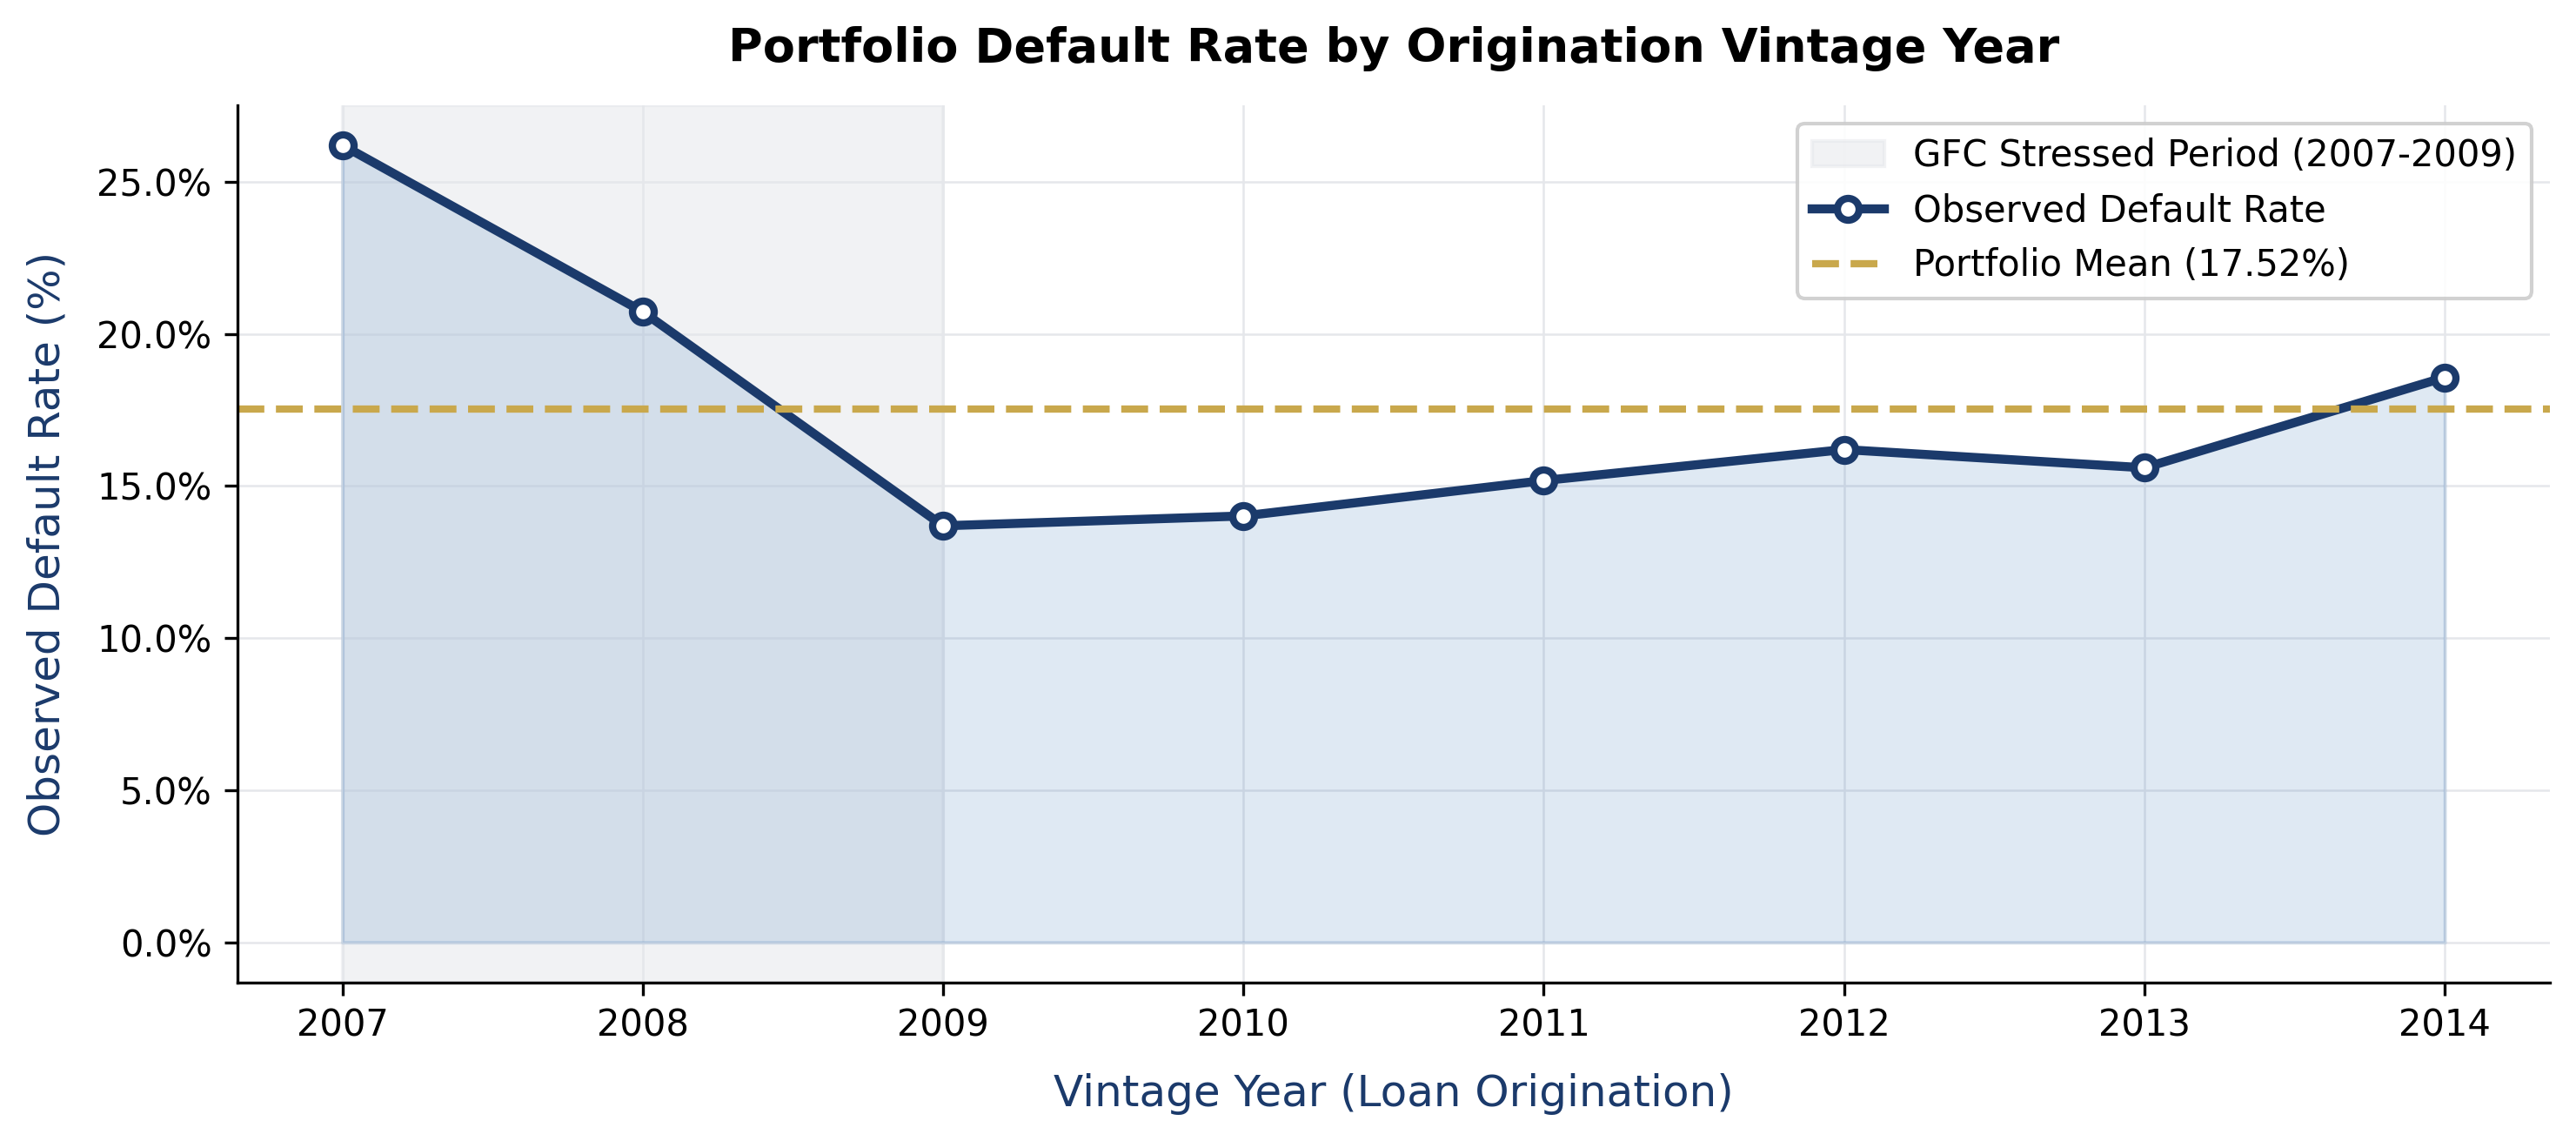
\includegraphics[width=0.65\textwidth]{figures/vintage_default_curves.png}
\caption{Cumulative Default Rates by Quarterly Vintage Cohorts}
\label{fig:vintage_curves}
\end{figure}

Figure~\ref{fig:eda_target_grade} displays additional exploratory distributions, demonstrating the relationship between historical default rates and risk grades, amortization terms, and loan purposes. Figure~\ref{fig:eda_dist_missing} completes the exploratory picture with the marginal distributions of the key numeric predictors and the missingness profile of the \emph{modelling} feature set --- that is, after the leakage deny-list has been applied in the loader, not the raw file. The distinction matters: the columns with the highest missingness in the raw LendingClub extract are the post-origination hardship and settlement blocks, which the deny-list removes before this figure is drawn, so describing it as the raw profile (as this passage previously did) points the reader at a different set of columns from the one plotted. The treatment applied to the remaining missing values is described in Section~3.1.

\begin{figure}[H]
\centering
\begin{subfigure}[b]{0.49\textwidth}
    \centering
    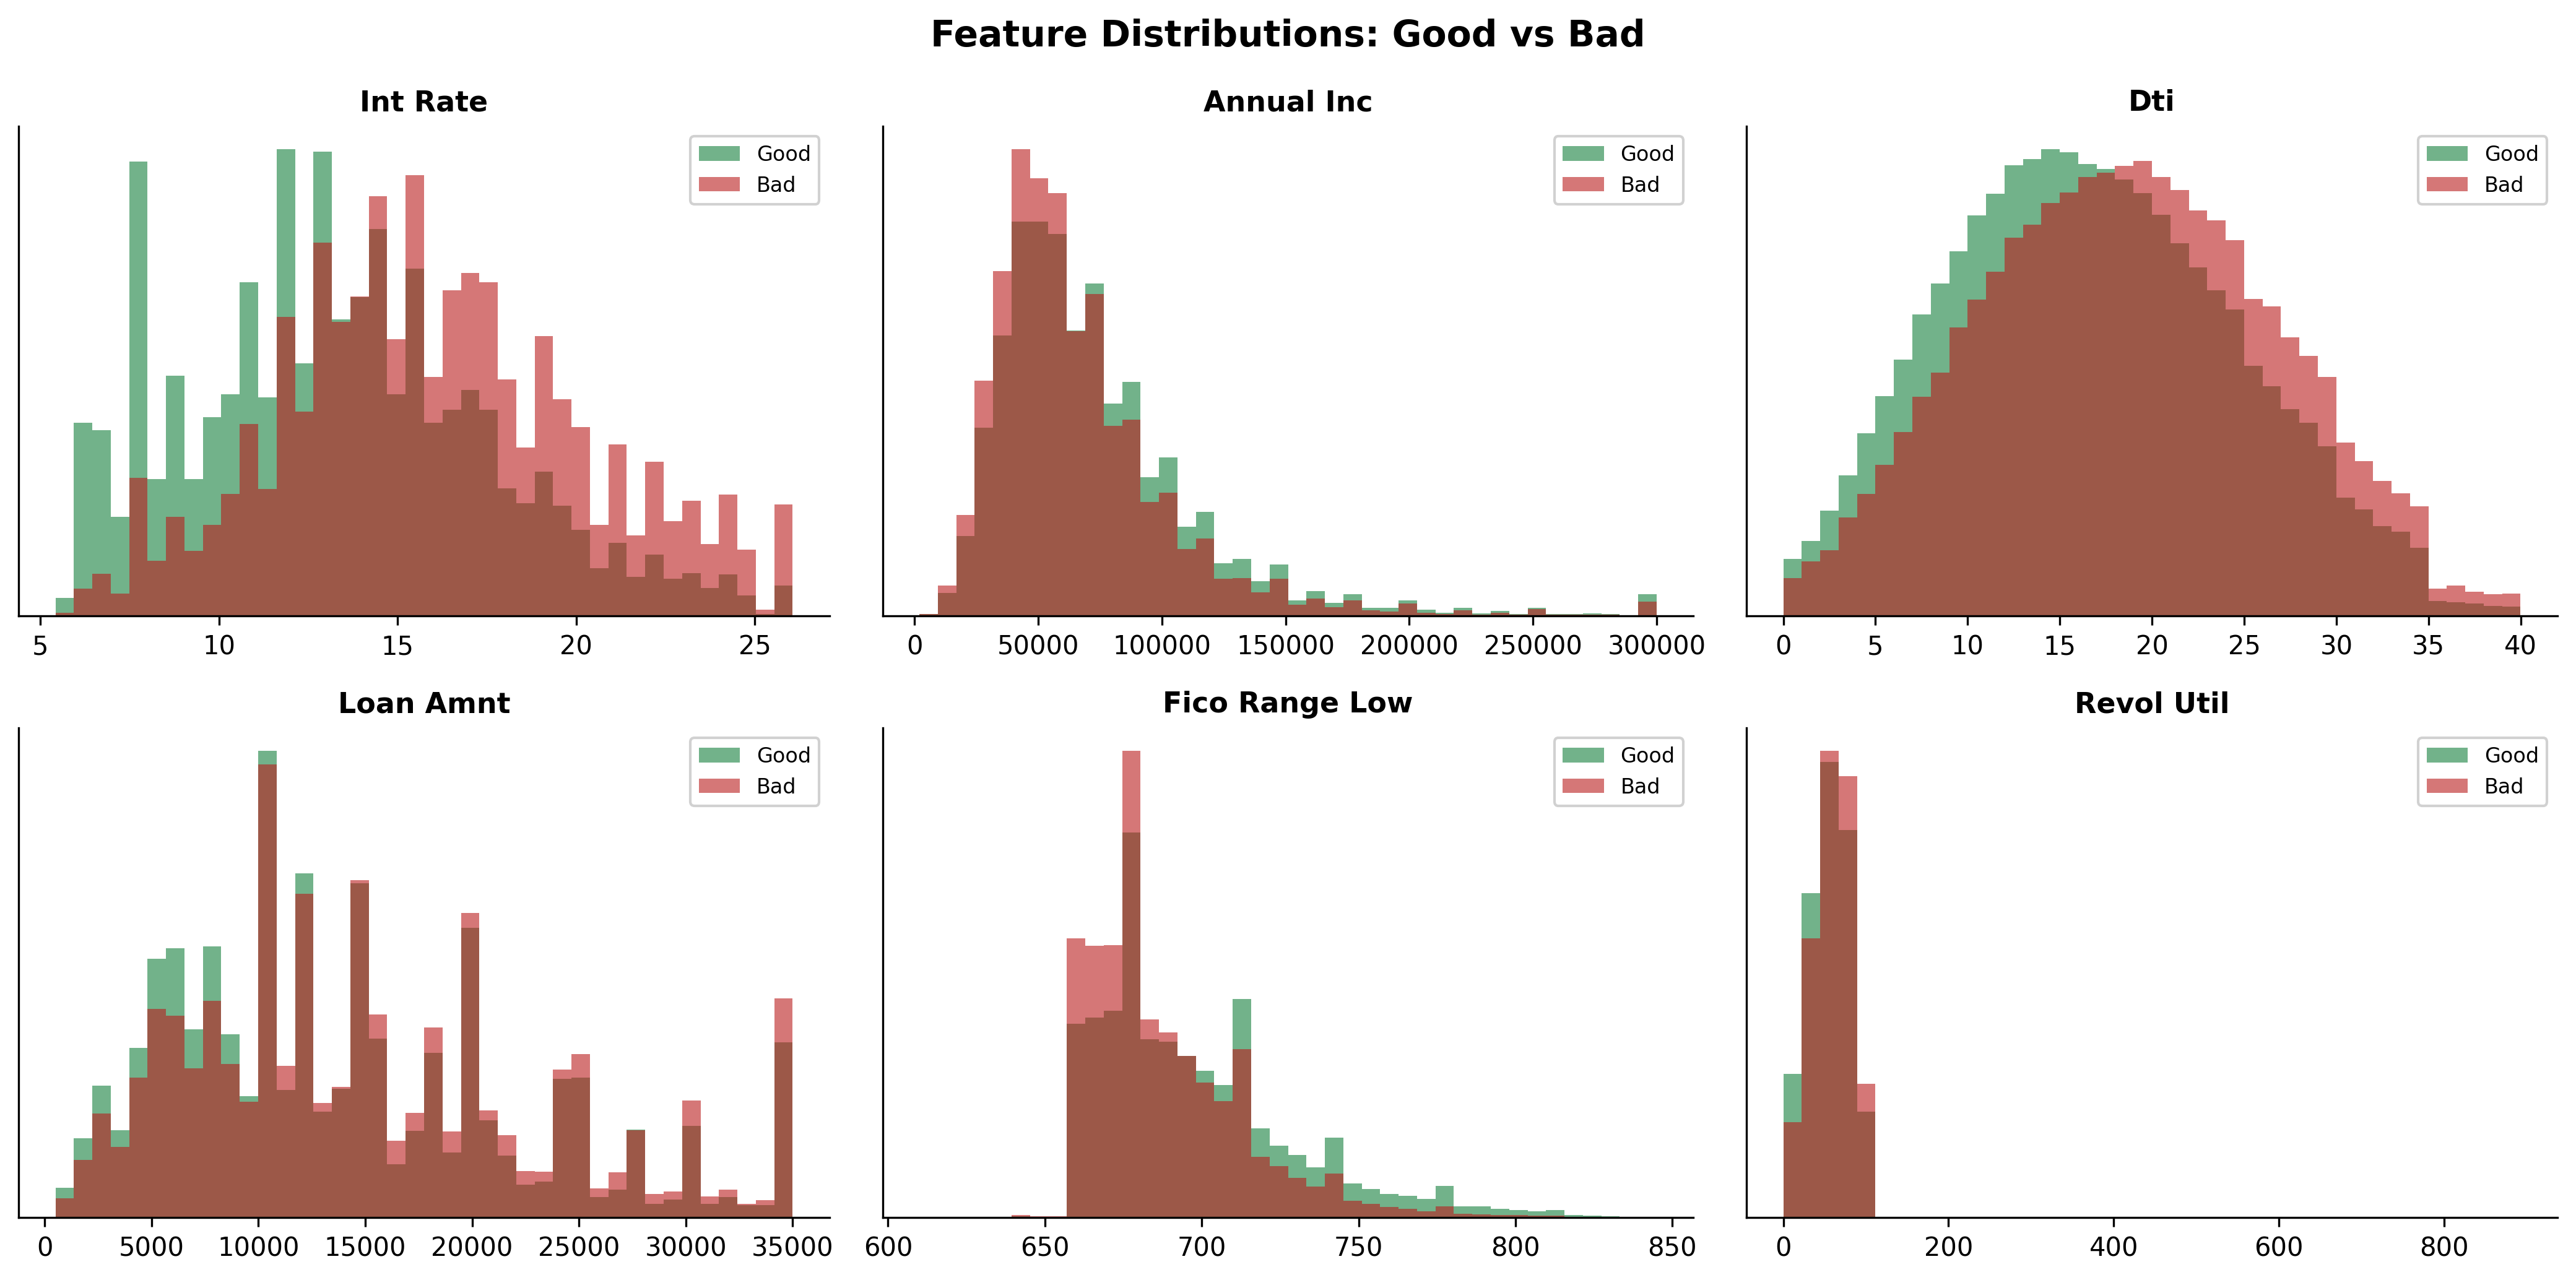
\includegraphics[width=\textwidth]{figures/numeric_distributions.png}
    \caption{Key numeric feature distributions}
    \label{fig:num_dist}
\end{subfigure}
\hfill
\begin{subfigure}[b]{0.49\textwidth}
    \centering
    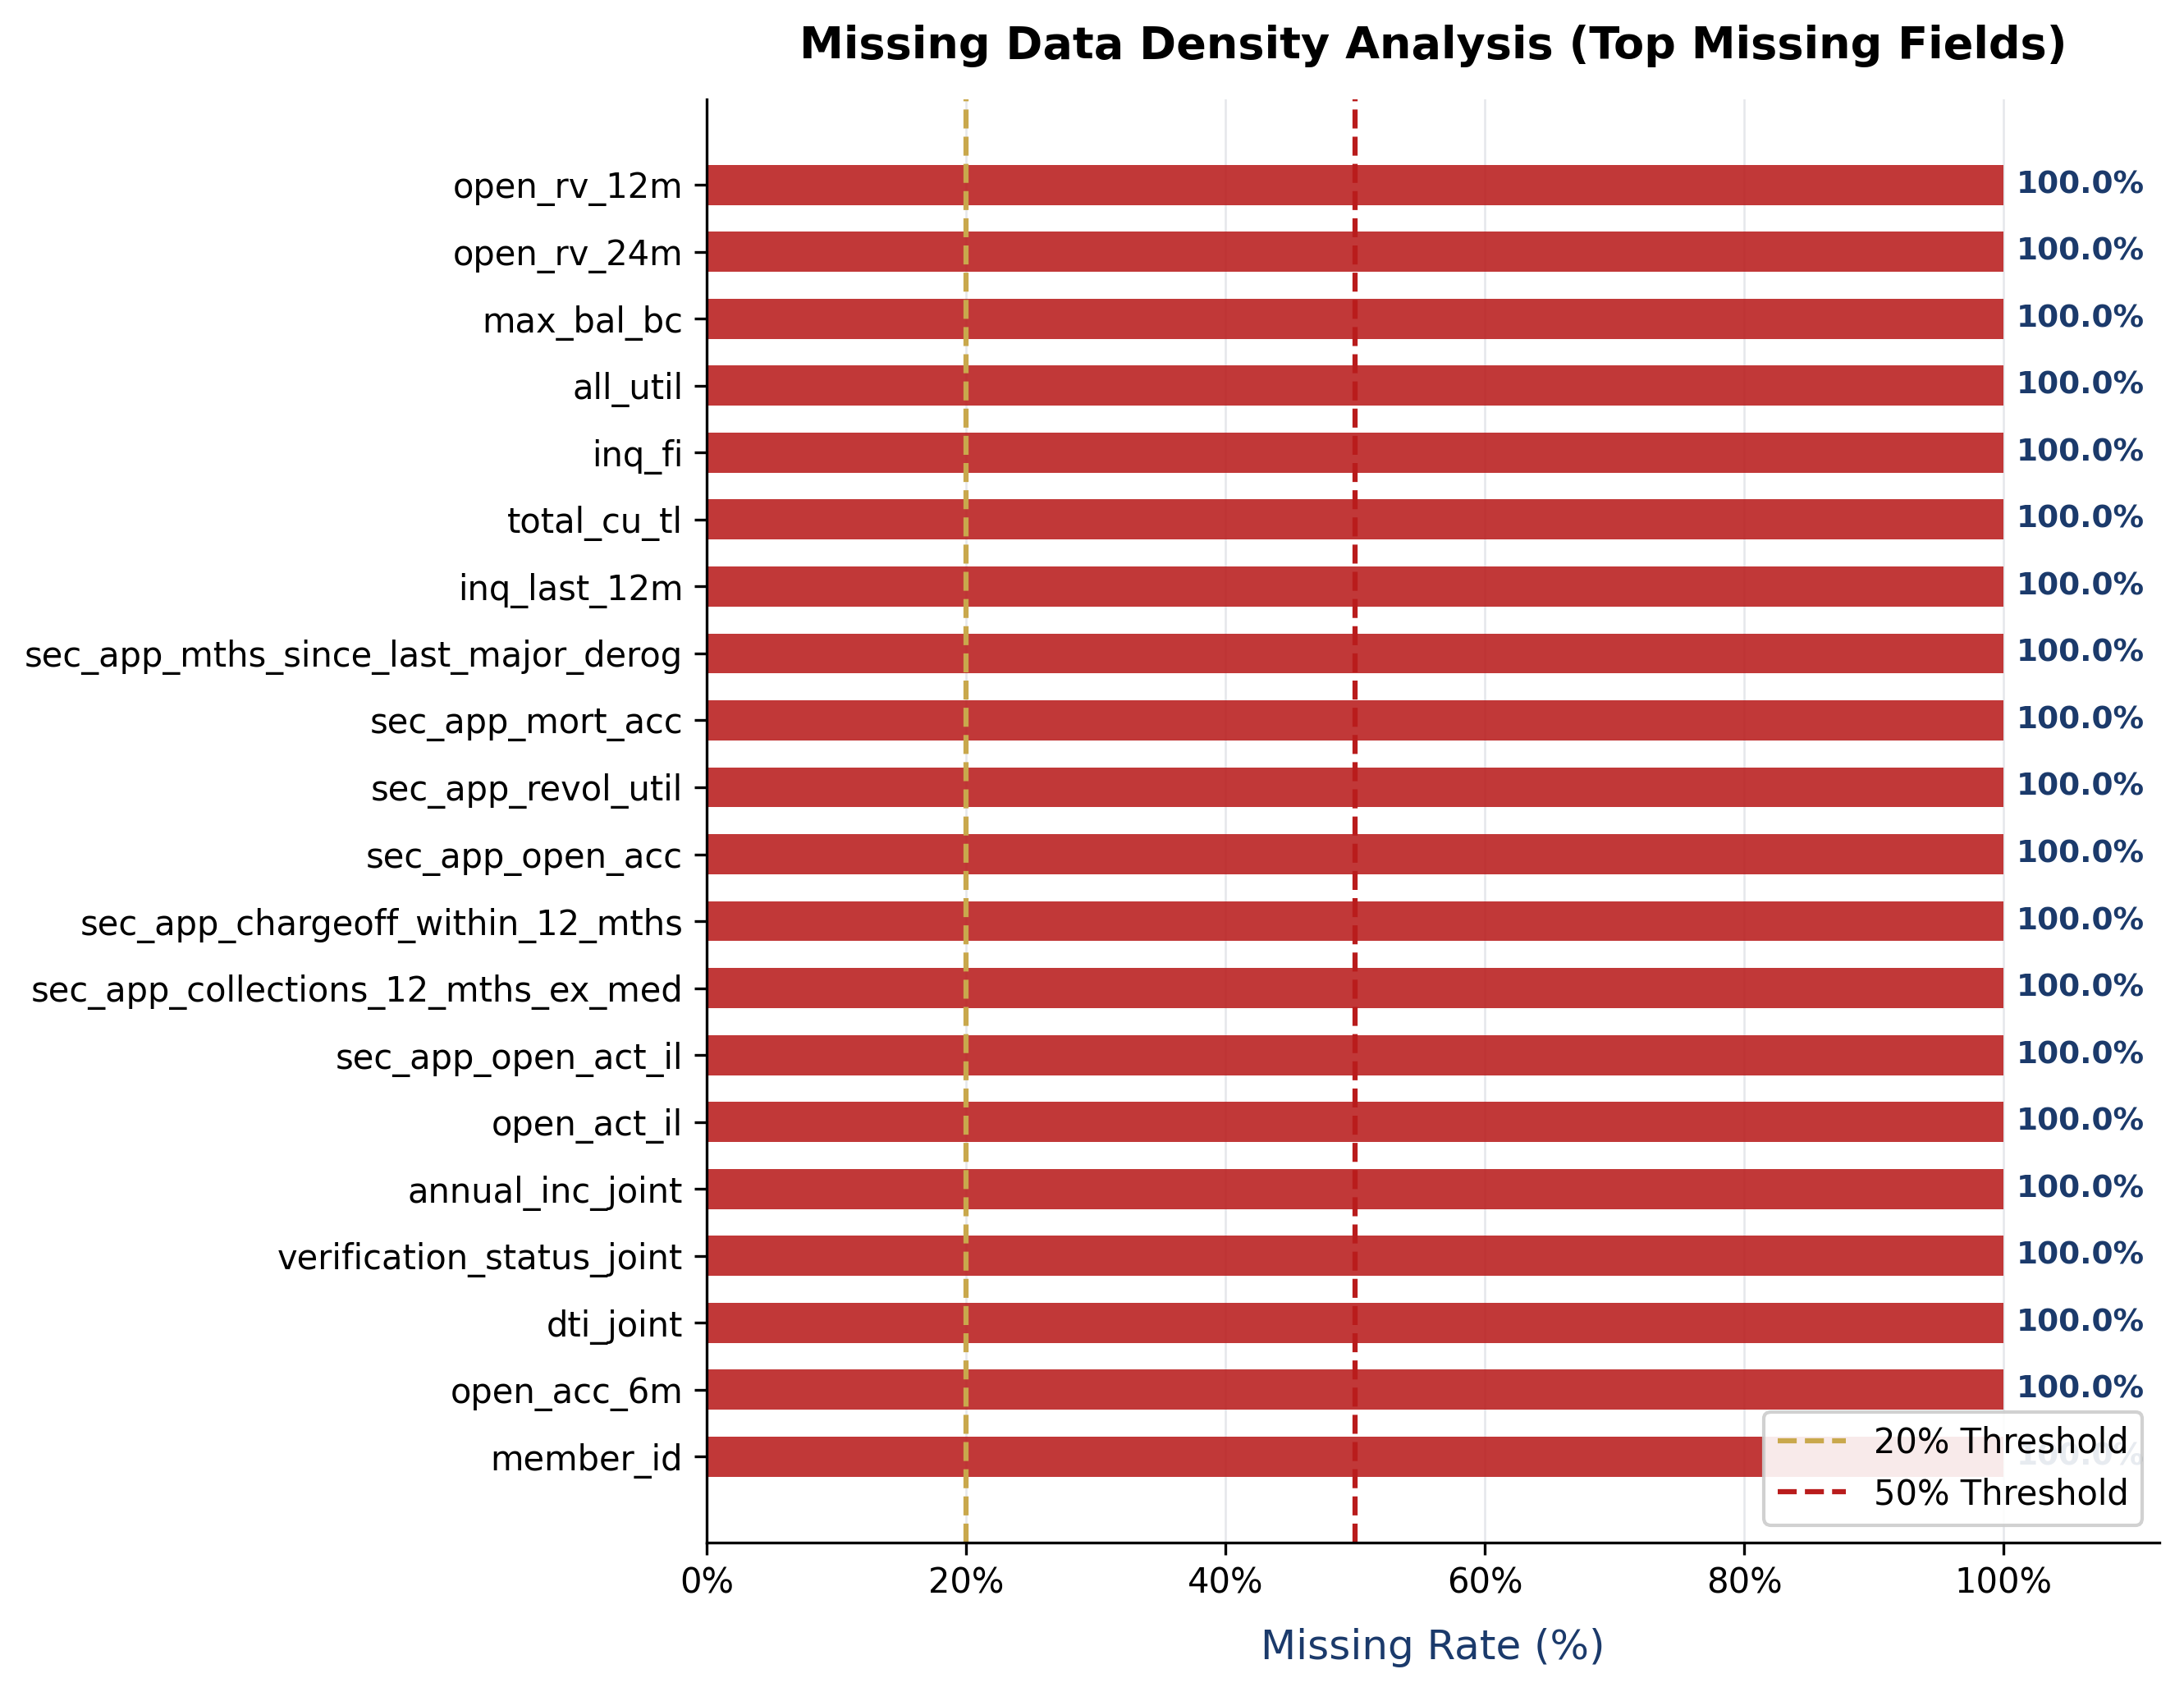
\includegraphics[width=\textwidth]{figures/missingness.png}
    \caption{Missingness density}
    \label{fig:missing_anal}
\end{subfigure}
\caption{Exploratory data analysis of the development sample: predictor distributions and missingness.}
\label{fig:eda_dist_missing}
\end{figure}

All EDA visualizations in this section are computed on the in-time development sample (train and test partitions of the resolved-outcome modelling population), not the full raw portfolio: the Out-of-Time partition is withheld from all exploratory analysis to preserve the integrity of the temporal validation, and loans with unresolved statuses are excluded per Section~2.1. Portfolio-level capital and impairment calculations are run on the modelling population ($N = $ 992,661), i.e.\ the train, test and OOT partitions combined --- not on the 2,260,701 loans in the source file, since loans with an unresolved status carry no good/bad label and are excluded (1,369,566 remain after that filter, of which 376,905 fall in the excluded grey zone described in Section~2.3). Population counts embedded in the EDA figures therefore reflect the development sample.

\begin{figure}[H]
\centering
\begin{subfigure}[b]{0.49\textwidth}
    \centering
    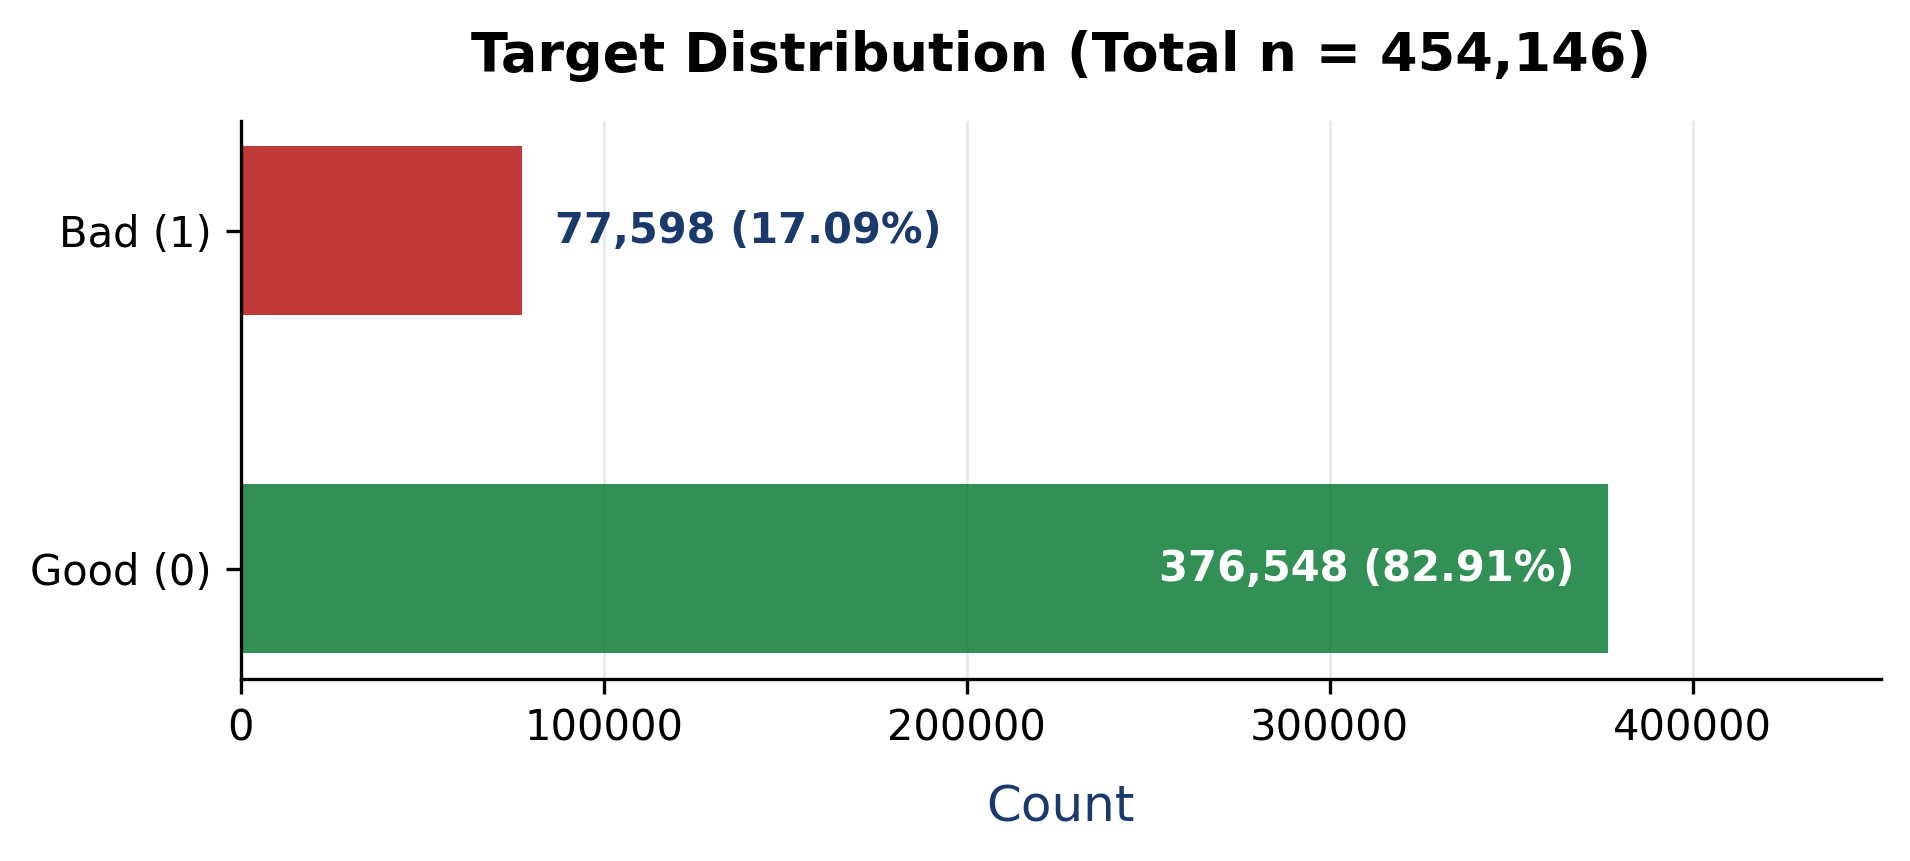
\includegraphics[width=\textwidth]{figures/target_distribution.png}
    \caption{Target Distribution (Good vs. Bad)}
    \label{fig:target_dist}
\end{subfigure}
\hfill
\begin{subfigure}[b]{0.49\textwidth}
    \centering
    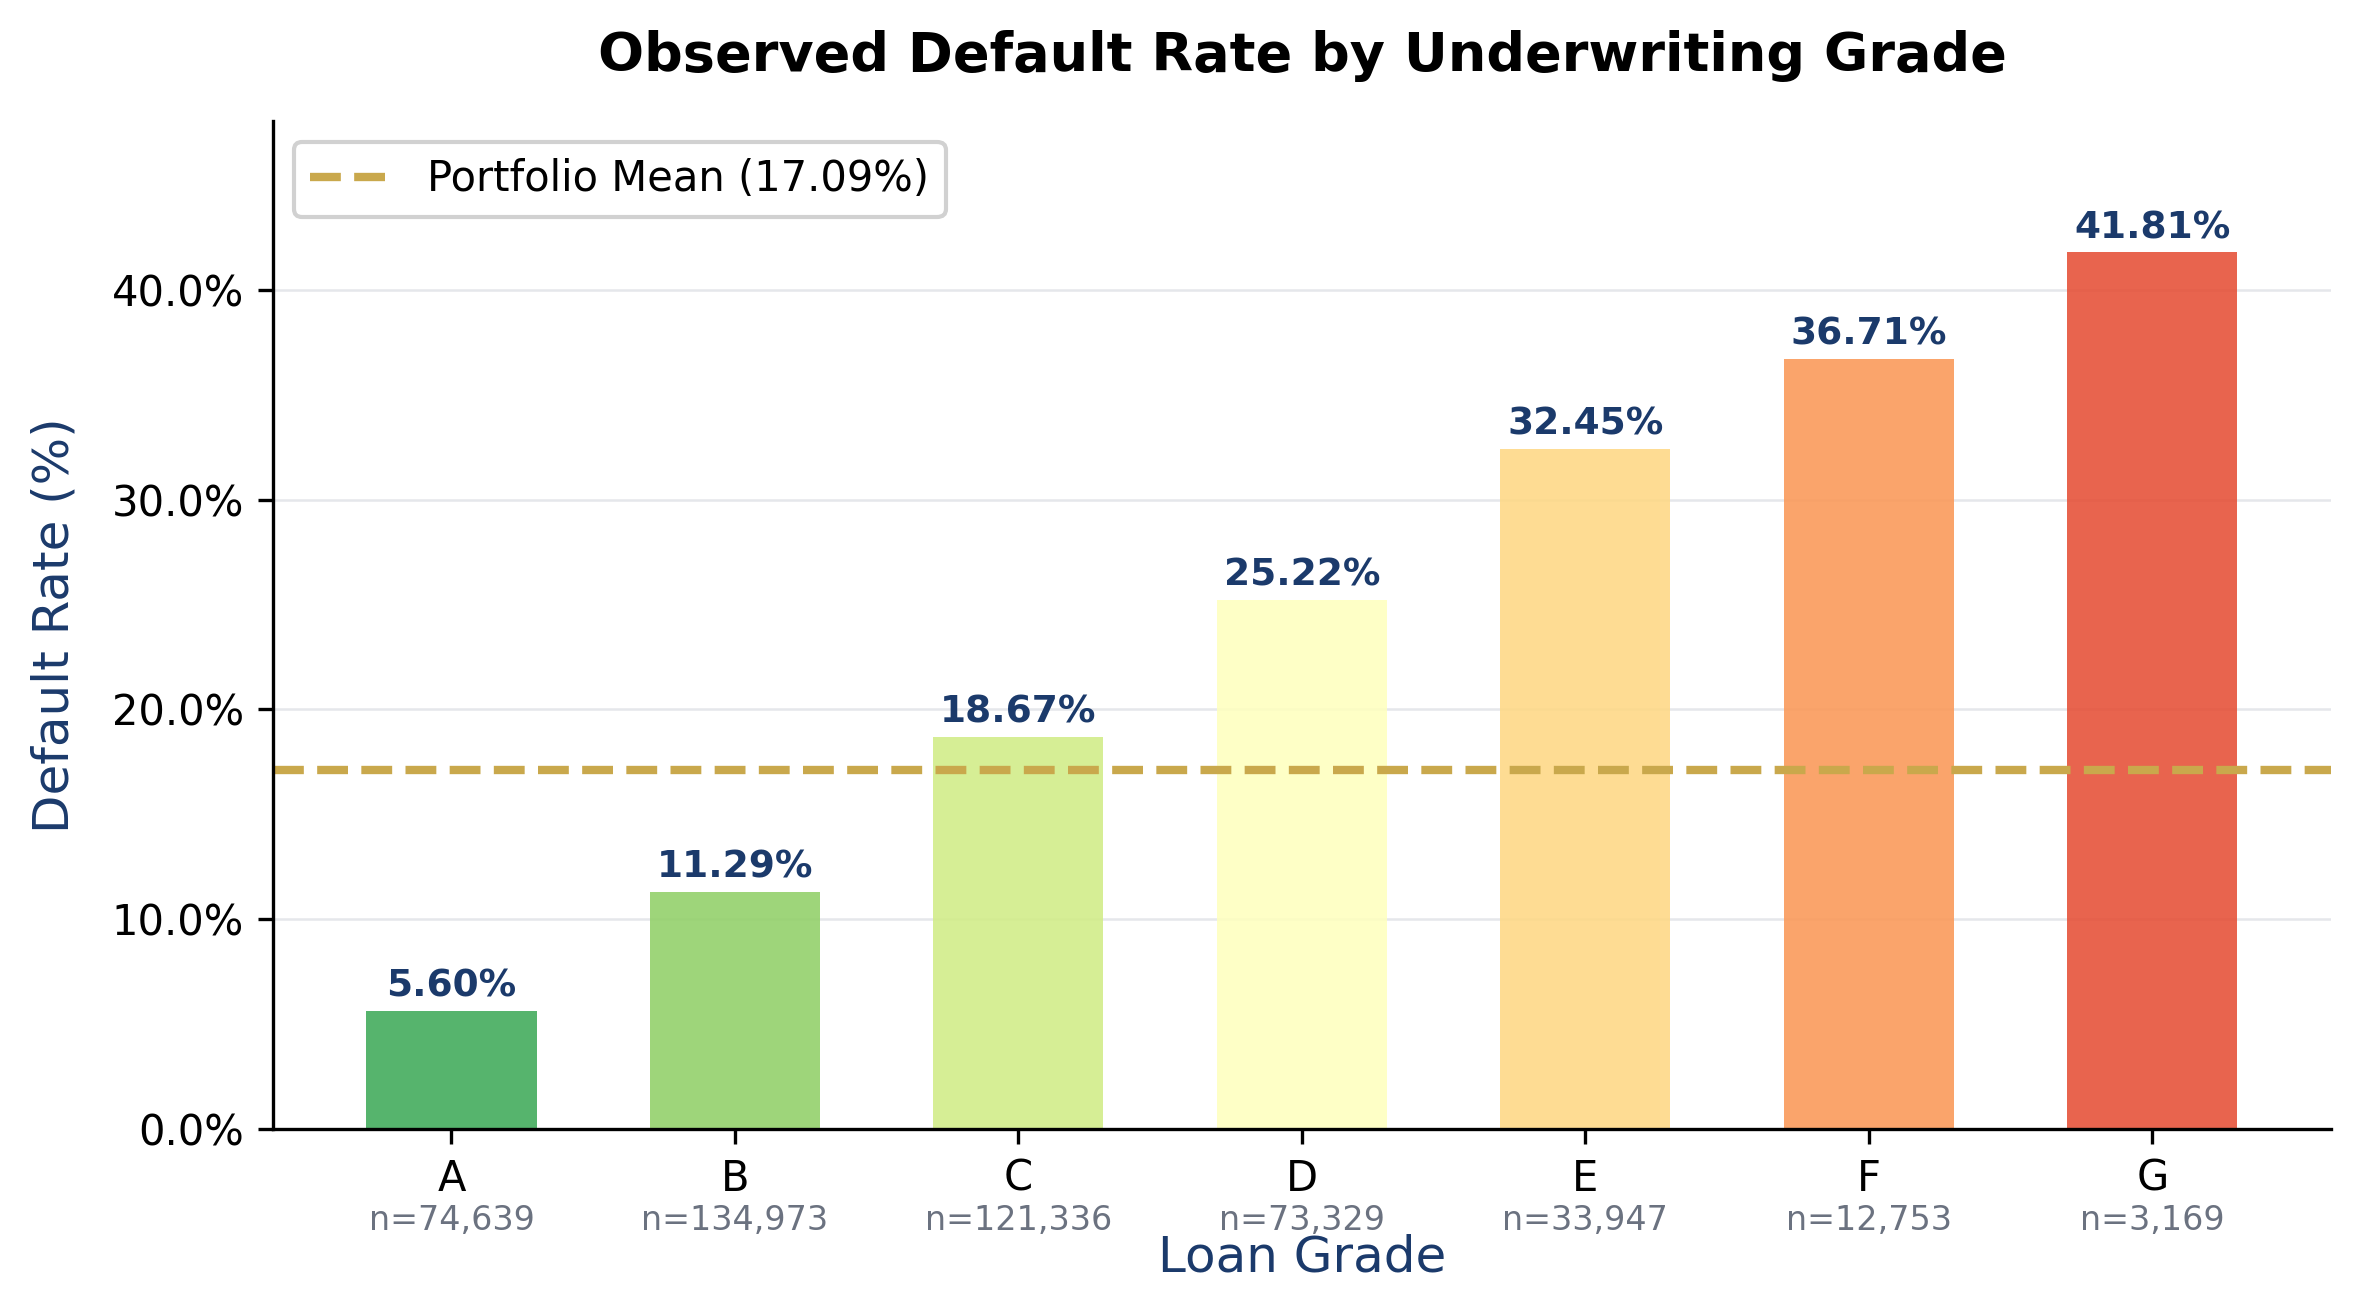
\includegraphics[width=\textwidth]{figures/default_rate_by_grade.png}
    \caption{Default Rate by Underwriting Grade}
    \label{fig:default_grade}
\end{subfigure}
\\[0.5em]
\begin{subfigure}[b]{0.49\textwidth}
    \centering
    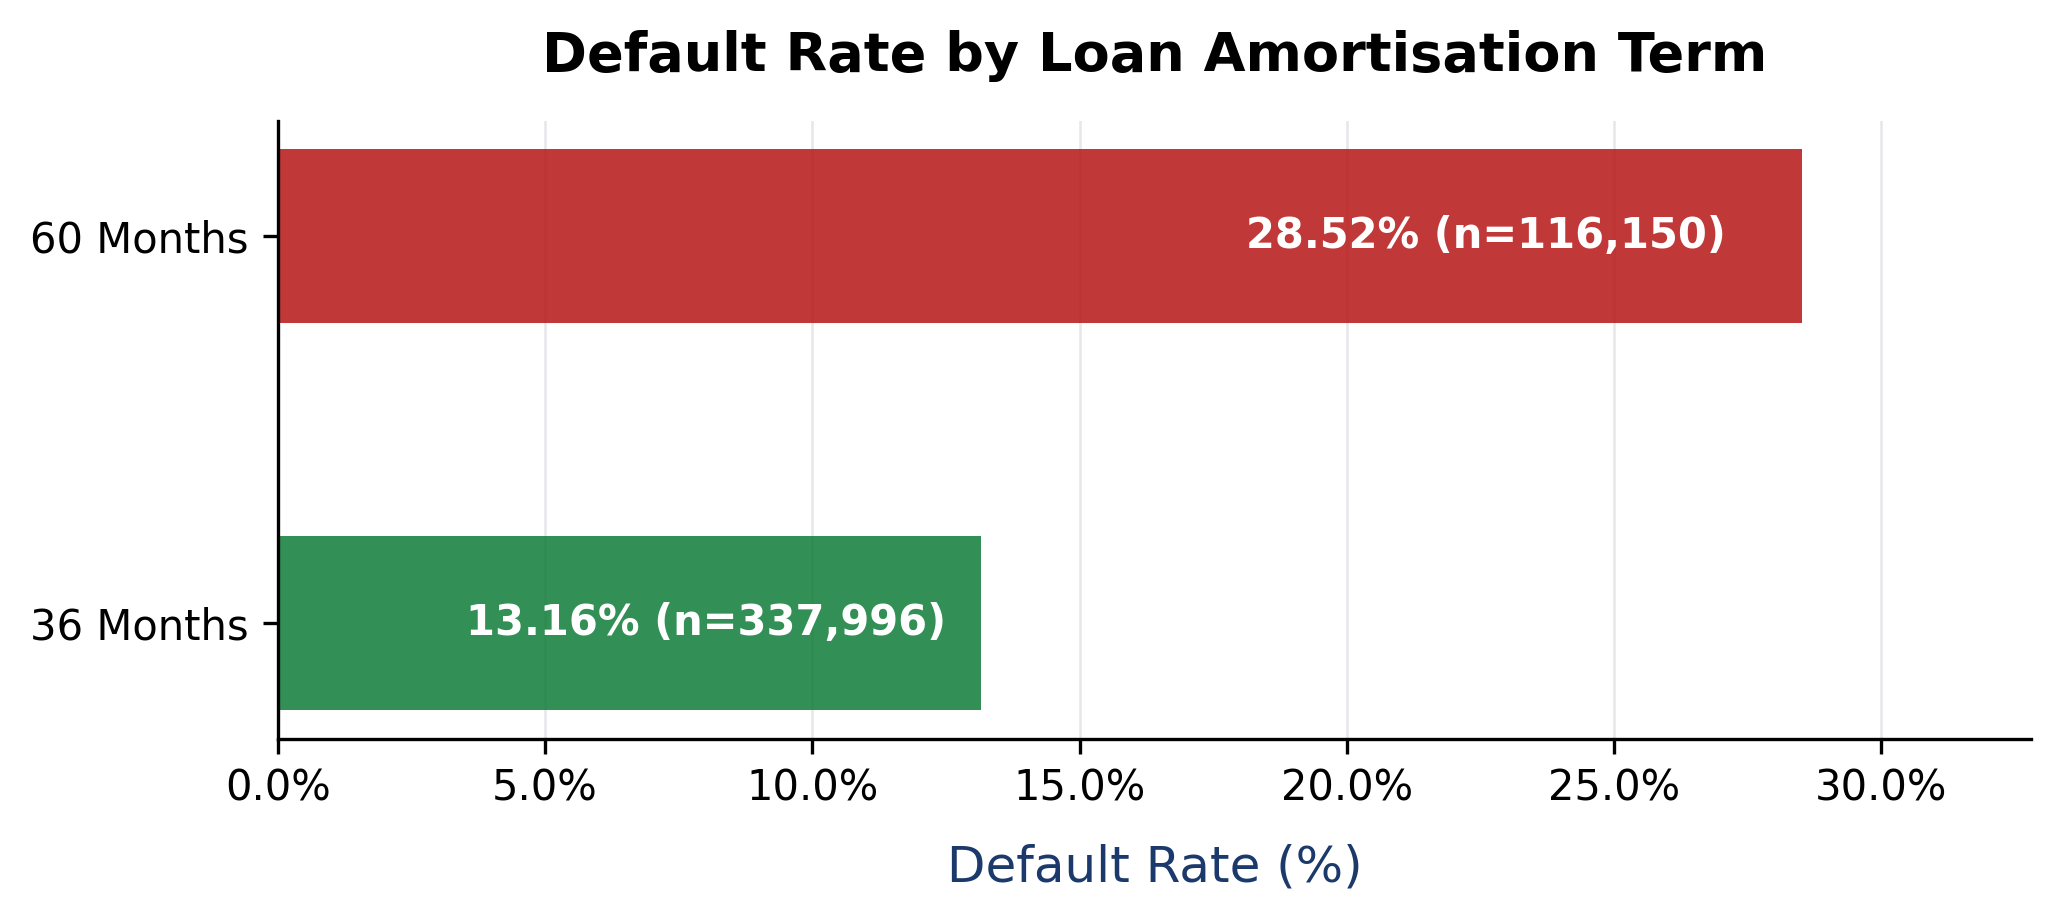
\includegraphics[width=\textwidth]{figures/default_rate_by_term.png}
    \caption{Default Rate by Amortisation Term}
    \label{fig:default_term}
\end{subfigure}
\hfill
\begin{subfigure}[b]{0.49\textwidth}
    \centering
    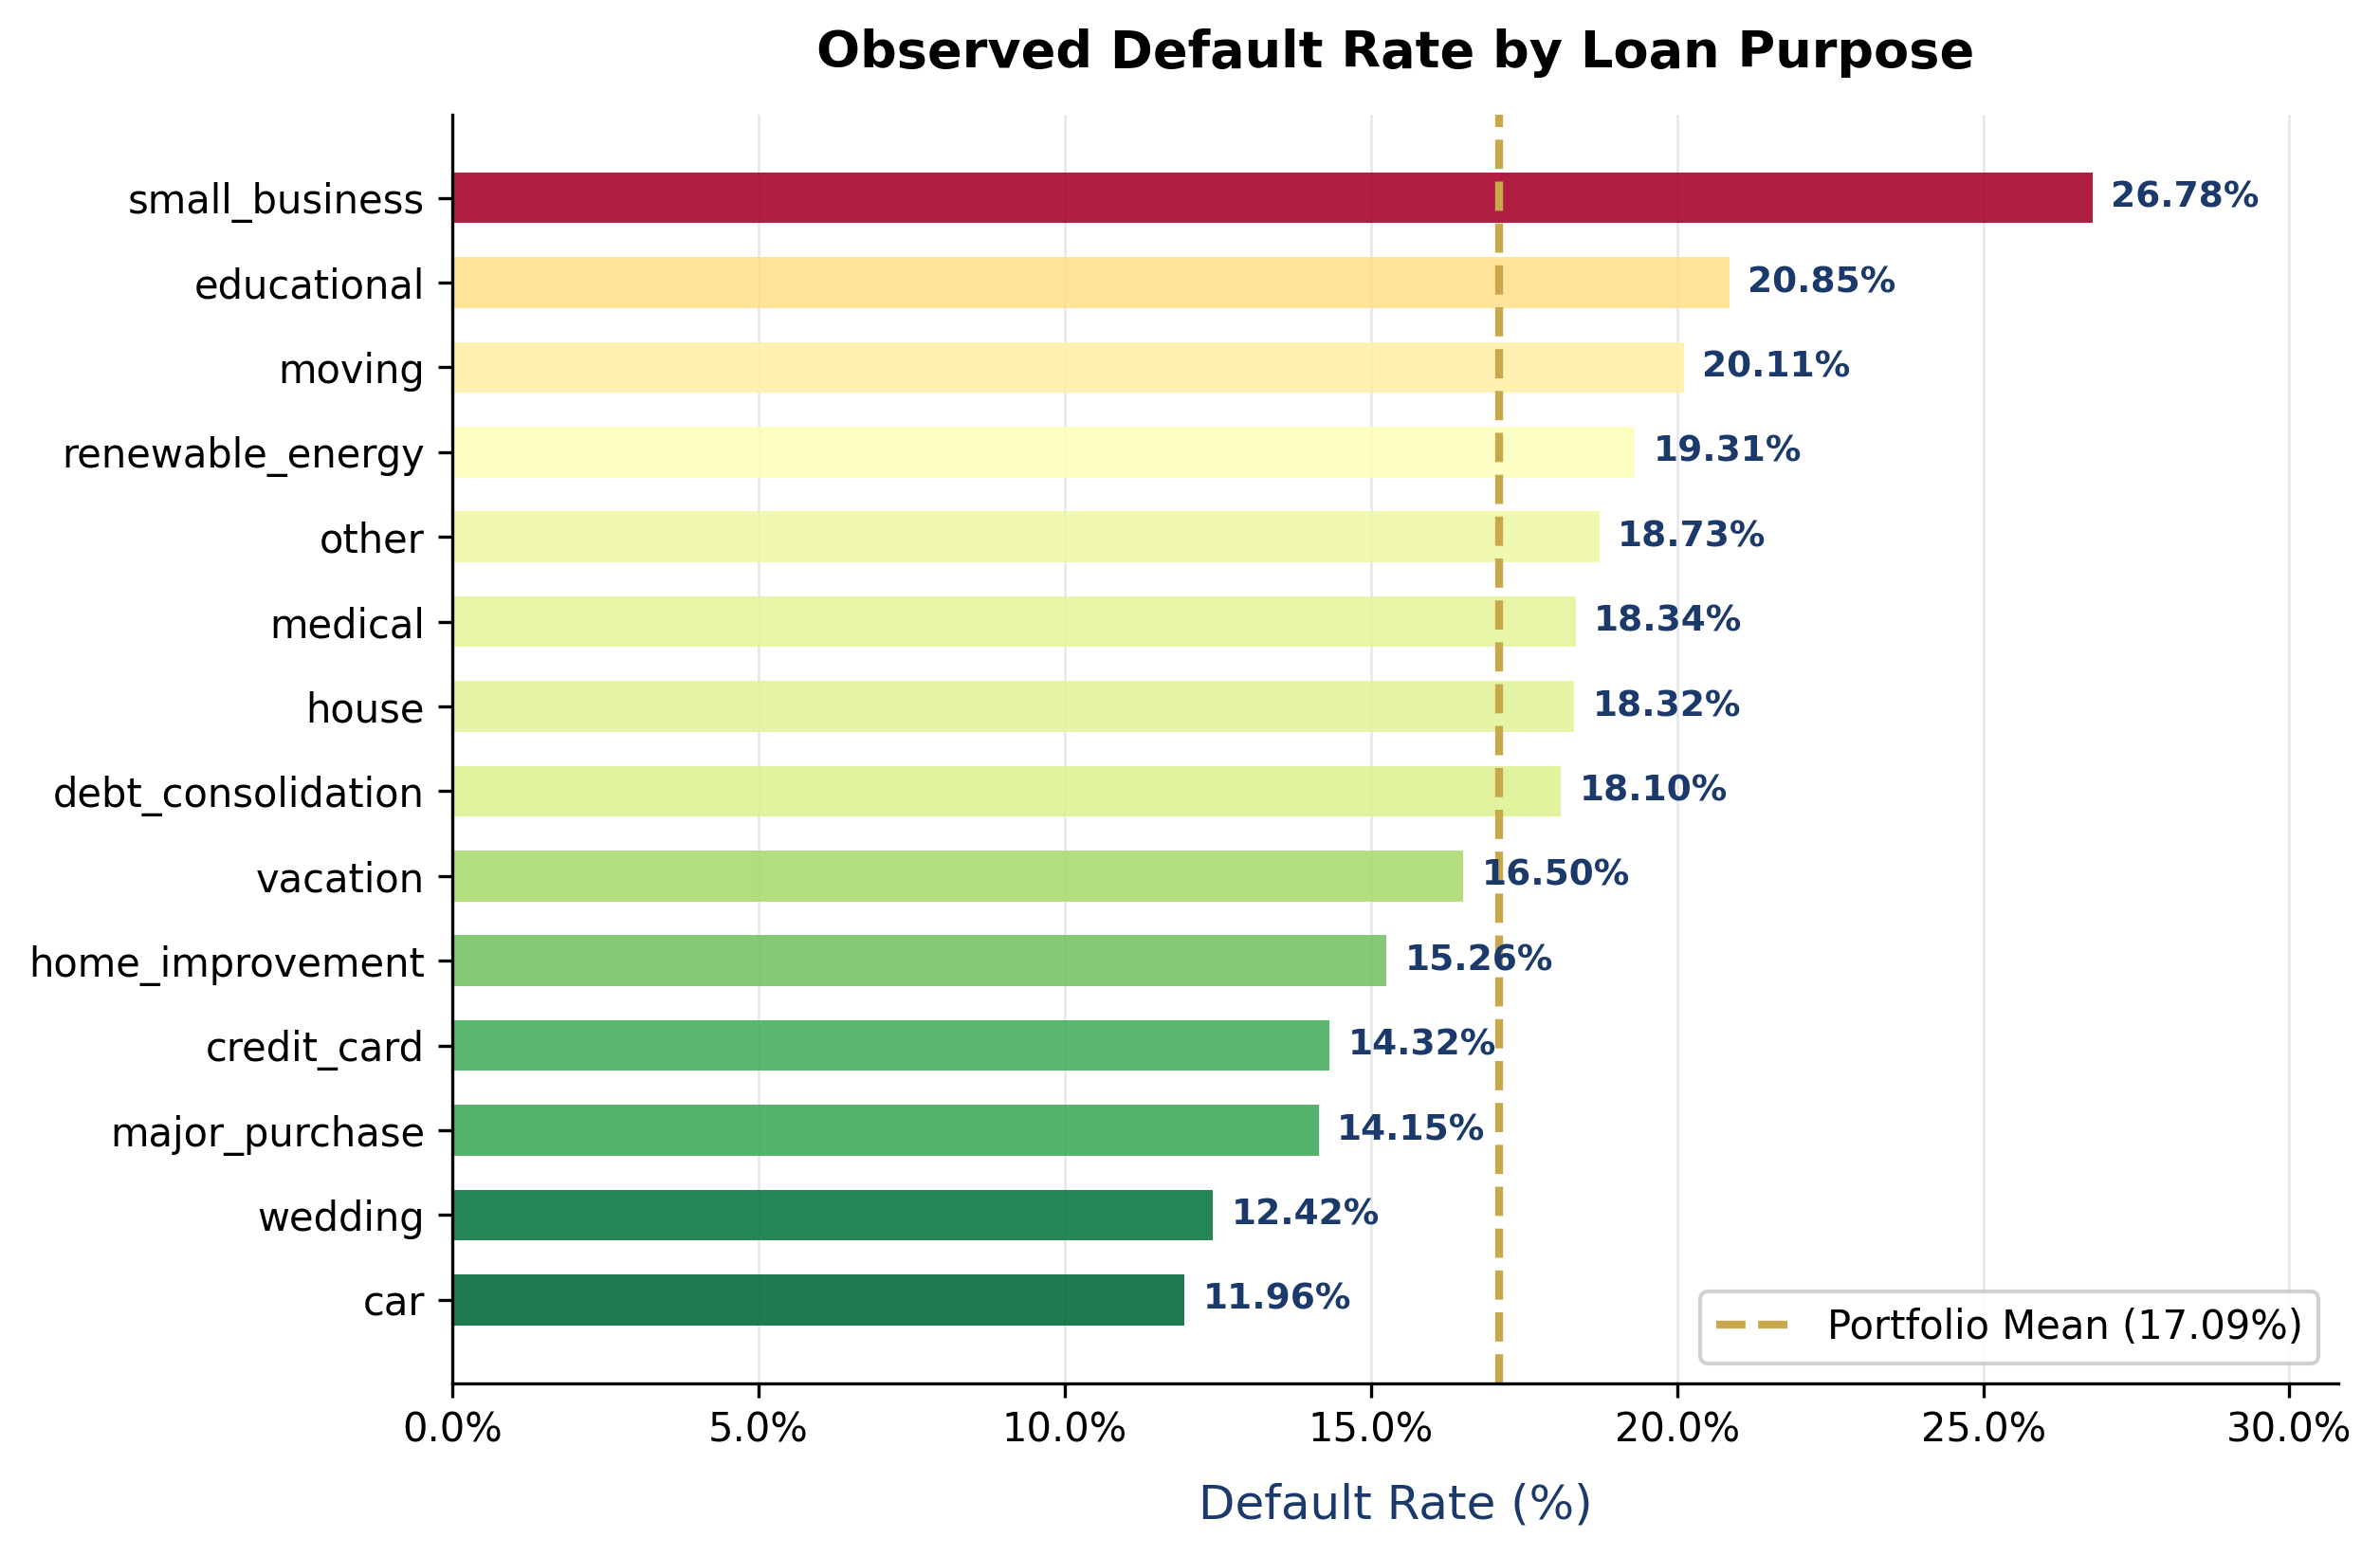
\includegraphics[width=\textwidth]{figures/default_rate_by_purpose.png}
    \caption{Default Rate by Loan Purpose}
    \label{fig:default_purpose}
\end{subfigure}
\caption{EDA Risk, Grade, Term, and Purpose Distributions}
\label{fig:eda_target_grade}
\end{figure}

% -----------------------------------------------------------------------------
% 3. PROBABILITY OF DEFAULT (PD) SCORECARD DEVELOPMENT
% -----------------------------------------------------------------------------
\section{Probability of Default (PD) Scorecard Development}

\subsection{Weight of Evidence (WoE) and Information Value (IV)}
Continuous features are binned to handle non-linear relationships, outliers, and missing values. Binning is performed by \texttt{optbinning}'s optimal-binning solver, which searches bin boundaries under a mixed-integer formulation; where the solver is unavailable the pipeline falls back to a quantile-split binner that merges adjacent bins until the sign of the WoE differences is homogeneous. Which of the two produced the bins reported here is recorded in Appendix~C. For each bin $i$, the Weight of Evidence (WoE) is calculated as:
\begin{equation}
WoE_i = \ln\!\left( \frac{\text{Proportion of Good}_i}{\text{Proportion of Bad}_i} \right) = \ln\!\left( \frac{N_{G,i} / N_{G,total}}{N_{B,i} / N_{B,total}} \right)
\end{equation}
The predictive power of each feature is evaluated using the Information Value (IV):
\begin{equation}
IV = \sum_{i=1}^{k} \left( \frac{N_{G,i}}{N_{G,total}} - \frac{N_{B,i}}{N_{B,total}} \right) \times WoE_i
\end{equation}
\parencite[Ch.~4]{siddiqi2017}; \parencite{hand1997}. Features with an IV below $0.02$ are dropped due to low predictive power, while multicollinearity is controlled by removing features with a Variance Inflation Factor (VIF) greater than $5.0$. Two further selection stages follow; the complete funnel is set out in Section~3.3.

\subsubsection*{Missing-value treatment}
Missing values are passed to the binner as missing and receive a bin of their own, with a Weight of Evidence estimated from the observed default rate among the missing rows. Their contribution to a borrower's score is therefore whatever the data says it is, and it is visible as a populated row in the points table rather than folded invisibly into another band.

This matters more than it may appear. An earlier version of this pipeline substituted the sentinel value $-9999$ before binning. That placed every missing observation in the extreme lower bin of its feature, with three consequences: the binner's own ``Missing'' bin was structurally empty and its code path never executed; the implied risk direction was arbitrary and inconsistent across features, since a missing value scored as \emph{worst} for a feature where low is risky (FICO, available credit) and as \emph{best} for one where low is safe (DTI, recent enquiries); and for \texttt{mths\_since\_recent\_bc}, where missing means the borrower has never held a bankcard, the assignment carried the wrong sign outright. Because the two binning implementations also handled the sentinel differently, they produced materially different models from identical data.

\subsection{Logistic Regression and Scorecard Scaling}
A regularized logistic regression \parencite{hosmer2013} is fitted on the WoE-transformed features. Since higher WoE corresponds to a higher proportion of ``Good'' loans relative to ``Bad'' loans, all coefficients must be negative when predicting default ($Y=1$). The scorecard is then scaled to a points-based system using:
\begin{equation}
Score = Offset + Factor \times \ln(\text{odds})
\end{equation}
\begin{equation}
Factor = \frac{PDO}{\ln(2)}, \quad Offset = TargetScore - Factor \times \ln(TargetOdds)
\end{equation}
For $TargetScore = 600$ points, $TargetOdds = 50:1$, and $PDO = 20$ (points to double the odds), the scaling parameters are:
\begin{itemize}
    \item $Factor = 28.8539$
    \item $Offset = 487.123$
\end{itemize}
The points contributed by a specific binned attribute $j$ are calculated as:
\begin{equation}
Points_j = \left( -(WoE_j \times \beta_j) + \frac{\alpha}{n} \right) \times Factor + \frac{Offset}{n}
\end{equation}
where $\beta_j$ is the regression coefficient, $\alpha$ is the model intercept, and $n$ is the number of active features \parencite[Ch.~5]{anderson2007}.

\subsection{Feature Selection Results: the Four-Stage Funnel}
After WoE binning, candidate features pass through \textbf{four} sequential filters, not two. Reporting only the first two would leave the final list unreconcilable with the IV ranking below --- several high-IV candidates are removed by the later stages:

\begin{enumerate}
    \item \textbf{IV band.} Features with $IV < 0.02$ (negligible predictive power) or $IV > 0.50$ (likely target leakage) are excluded.
    \item \textbf{VIF filter.} Multicollinearity is controlled by iteratively removing features with a Variance Inflation Factor above 5.0.
    \item \textbf{ElasticNet shrinkage.} A cross-validated penalised logistic regression (\texttt{LogisticRegressionCV}, SAGA solver, $\ell_1$ ratio $0.5$, 3-fold stratified CV) is fitted on the survivors, and features whose coefficient shrinks to $|\beta| \le 10^{-4}$ are dropped. This stage removes predictors that are individually informative but redundant given the rest of the set --- which is why a high-IV variable can be absent from the final list.
    \item \textbf{Sign check.} The unpenalised logistic regression is fitted and any feature whose coefficient carries the wrong sign (positive on a WoE predictor, i.e.\ higher WoE implying higher default risk) is dropped, and the model refitted on the survivors.
\end{enumerate}

\noindent The funnel for this run: 81 candidate features $\rightarrow$ 37 after the IV band $[0.02, 0.50]$ $\rightarrow$ 25 after the VIF filter $\rightarrow$ 22 after ElasticNet shrinkage $\rightarrow$ \textbf{16} after the sign check. Dropped by the sign check: \texttt{bc\_util}, \texttt{mo\_sin\_rcnt\_rev\_tl\_op}, \texttt{mo\_sin\_rcnt\_tl}, \texttt{revol\_util\_x\_open\_acc}, \texttt{tot\_cur\_bal}, \texttt{total\_rev\_hi\_lim}.

\begin{sloppypar}\noindent
The final set is: \texttt{grade\_enc},\allowbreak \texttt{term\_enc},\allowbreak \texttt{loan\_to\_income},\allowbreak \texttt{fico\_range\_high},\allowbreak \texttt{revol\_util\_x\_new\_acc},\allowbreak \texttt{new\_accounts\_ratio},\allowbreak \texttt{dti},\allowbreak \texttt{bc\_open\_to\_buy},\allowbreak \texttt{num\_tl\_op\_past\_12m},\allowbreak \texttt{log\_annual\_inc},\allowbreak \texttt{avg\_cur\_bal},\allowbreak \texttt{mths\_since\_recent\_inq},\allowbreak \texttt{inq\_last\_6mths\_per\_month},\allowbreak \texttt{num\_rev\_tl\_bal\_gt\_0},\allowbreak \texttt{mths\_since\_recent\_bc},\allowbreak \texttt{mort\_acc}.
\end{sloppypar}

\begin{table}[H]
\centering
\small
\caption{Feature Information Value (IV) Ranking (top 15)}
\label{tab:iv_ranking}
\vspace{0.5em}
\begin{tabular}{lccl}
\toprule
\textbf{Feature} & \textbf{IV} & \textbf{Predictive Power} & \textbf{Outcome} \\
\midrule
\texttt{int\_rate} & 0.4072 & Strong & Dropped (VIF) \\
\texttt{grade\_enc} & 0.3963 & Strong & \textbf{Retained} \\
\texttt{term} & 0.1998 & Medium & Dropped (VIF) \\
\texttt{term\_enc} & 0.1998 & Medium & \textbf{Retained} \\
\texttt{loan\_to\_income} & 0.1224 & Medium & \textbf{Retained} \\
\texttt{fico\_range\_low} & 0.1143 & Medium & Dropped (VIF) \\
\texttt{fico\_range\_high} & 0.1143 & Medium & \textbf{Retained} \\
\texttt{revol\_util\_x\_new\_acc} & 0.0969 & Weak & \textbf{Retained} \\
\texttt{total\_debt\_to\_income} & 0.0650 & Weak & Dropped (ElasticNet) \\
\texttt{new\_accounts\_ratio} & 0.0648 & Weak & \textbf{Retained} \\
\texttt{dti} & 0.0555 & Weak & \textbf{Retained} \\
\texttt{acc\_open\_past\_24mths} & 0.0543 & Weak & Dropped (VIF) \\
\texttt{bc\_open\_to\_buy} & 0.0519 & Weak & \textbf{Retained} \\
\texttt{num\_tl\_op\_past\_12m} & 0.0403 & Weak & \textbf{Retained} \\
\texttt{annual\_inc} & 0.0365 & Weak & Dropped (VIF) \\
\bottomrule
\multicolumn{4}{p{0.92\linewidth}}{\footnotesize \textit{Note:} the remaining 22 candidate features all carry IV $\le$ 0.0365 and are omitted; the full ranking is in \texttt{outputs/scorecard\_tables.json}. The \textit{Outcome} column names the stage of the four-stage funnel (Section~3.3) at which each feature left, which is why a high-IV feature can be absent from the final model. Monotone transforms of the same underlying variable (for example a raw and a log-scaled version) carry near-identical IV by construction and are not independent evidence.} \\
\end{tabular}
\end{table}

\subsection{Logistic Regression Coefficient Output}
The following table presents the logistic regression coefficient estimates, standard errors, z-statistics and p-values for all retained features. As expected for a WoE-based model predicting default ($Y=1$), all feature coefficients carry a \textbf{negative sign}: higher WoE values indicate a higher proportion of ``Good'' loans, and therefore map to lower default probability.

\begin{table}[H]
\centering
\caption{Logistic Regression Coefficient Summary}
\label{tab:logit_coefficients}
\vspace{0.5em}
\begin{tabular}{lcccc}
\toprule
\textbf{Feature} & \textbf{Coefficient} & \textbf{Std.\ Error} & \textbf{z-stat} & \textbf{p-value} \\
\midrule
\texttt{const} & -1.6110 & 0.0053 & -303.072 & 0.0000$^{***}$ \\
\texttt{grade\_enc} & -0.5155 & 0.0106 & -48.618 & 0.0000$^{***}$ \\
\texttt{term\_enc} & -0.6521 & 0.0125 & -51.995 & 0.0000$^{***}$ \\
\texttt{loan\_to\_income} & -0.4489 & 0.0158 & -28.416 & 0.0000$^{***}$ \\
\texttt{fico\_range\_high} & -0.2674 & 0.0190 & -14.091 & 0.0000$^{***}$ \\
\texttt{revol\_util\_x\_new\_acc} & -0.0486 & 0.0240 & -2.021 & 0.0433$^{**}$ \\
\texttt{new\_accounts\_ratio} & -0.4533 & 0.0260 & -17.409 & 0.0000$^{***}$ \\
\texttt{dti} & -0.3297 & 0.0221 & -14.908 & 0.0000$^{***}$ \\
\texttt{bc\_open\_to\_buy} & -0.3960 & 0.0272 & -14.576 & 0.0000$^{***}$ \\
\texttt{num\_tl\_op\_past\_12m} & -0.2197 & 0.0302 & -7.279 & 0.0000$^{***}$ \\
\texttt{log\_annual\_inc} & -0.4578 & 0.0325 & -14.077 & 0.0000$^{***}$ \\
\texttt{avg\_cur\_bal} & -0.3561 & 0.0334 & -10.668 & 0.0000$^{***}$ \\
\texttt{mths\_since\_recent\_inq} & -0.0260 & 0.0516 & -0.505 & 0.6137 \\
\texttt{inq\_last\_6mths\_per\_month} & -0.5131 & 0.0400 & -12.837 & 0.0000$^{***}$ \\
\texttt{num\_rev\_tl\_bal\_gt\_0} & -0.3303 & 0.0347 & -9.521 & 0.0000$^{***}$ \\
\texttt{mths\_since\_recent\_bc} & -0.3733 & 0.0367 & -10.159 & 0.0000$^{***}$ \\
\texttt{mort\_acc} & -0.3904 & 0.0424 & -9.212 & 0.0000$^{***}$ \\
\midrule
\multicolumn{5}{l}{\footnotesize Significance: $^{***}p<0.01$, $^{**}p<0.05$, $^{*}p<0.10$} \\
\bottomrule
\end{tabular}
\end{table}

\subsection{Scorecard Points Table}
Each WoE bin is converted to credit score points using the scaling formula. Higher points correspond to lower default risk. The table below shows the top bins ranked by point spread (i.e., the features with the greatest discriminatory contribution to the final score).

\begin{table}[H]
\centering
\small
\caption{Credit Scorecard Points Table --- complete bin ladders for the highest-spread features}
\label{tab:scorecard_points}
\vspace{0.5em}
\begin{tabular}{llccrrr}
\toprule
\textbf{Feature} & \textbf{Bin} & \textbf{WoE} & \textbf{$\beta$} & \textbf{N} & \textbf{DR\%} & \textbf{Points} \\
\midrule
\texttt{grade\_enc} & (-inf, 1.50) & 1.2418 & -0.5155 & 59,675 & 5.62\% & 51.8 \\
\texttt{} & [1.50, 2.50) & 0.4866 & -0.5155 & 107,931 & 11.25\% & 40.6 \\
\texttt{} & [2.50, 3.50) & -0.1063 & -0.5155 & 96,905 & 18.65\% & 31.8 \\
\texttt{} & [3.50, 4.50) & -0.4971 & -0.5155 & 58,848 & 25.31\% & 26.0 \\
\texttt{} & [4.50, inf) & -0.9212 & -0.5155 & 39,958 & 34.12\% & 19.6 \\
\texttt{} & Special & 0.0000 & -0.5155 & 0 & 0.00\% & 33.4 \\
\texttt{} & Missing & 0.0000 & -0.5155 & 0 & 0.00\% & 33.4 \\
\texttt{term\_enc} & (-inf, 48.00) & 0.3076 & -0.6521 & 270,363 & 13.16\% & 39.1 \\
\texttt{} & [48.00, inf) & -0.6604 & -0.6521 & 92,954 & 28.52\% & 20.9 \\
\texttt{} & Special & 0.0000 & -0.6521 & 0 & 0.00\% & 33.4 \\
\texttt{} & Missing & 0.0000 & -0.6521 & 0 & 0.00\% & 33.4 \\
\bottomrule
\multicolumn{7}{p{0.92\linewidth}}{\footnotesize WoE = ln(\%Good/\%Bad); Points = ($-\text{WoE}_j * \beta_j + \alpha/n$) * Factor + Offset/n. The remaining 14 scorecard features follow the same construction; their complete ladders are in \texttt{outputs/scorecard\_tables.json}. Where a calibrator is attached in production, the score-to-PD mapping tabulated here is the \emph{pre-recalibration} relationship: the points scale is built from the raw logit so that it stays additive and auditable, while the deployed PD passes through the recalibration transform of Section~7.2.} \\
\end{tabular}
\end{table}

\subsection{Interpretability vs.\ Performance: Challenger Model Benchmark}
A non-linear LightGBM model was trained as a challenger \parencite{baesens2016} on the scorecard's selected predictors (see Section~7.8 for the exact feature count actually consumed by each model). Although gradient boosting is competitive in-sample, on the out-of-time set the best challenger, Weighted Ensemble, \emph{exceeds} the scorecard's discrimination (OOT AUC 0.7037 vs 0.7003), a gap tested in Section~7.8. The scorecard is nonetheless retained as the production model for regulatory and explainability reasons set out below, with the discrimination sacrifice reported rather than obscured. Regulatory standards (such as the US Fair Credit Reporting Act) require financial institutions to provide clear ``adverse action codes'' (reasons for denial) to rejected applicants. A linear scorecard allows for immediate, exact points-attribution for each feature, which is not possible with complex machine learning models without relying on approximations like SHAP.

To address potential policy-decision circularity from using LendingClub's own underwriting variables (\texttt{int\_rate} and \texttt{grade}), we developed a secondary Pure Underwriting Scorecard (Model B). Model B excludes \texttt{int\_rate}, \texttt{grade\_enc}, \texttt{grade}, \texttt{sub\_grade}, \texttt{sub\_grade\_enc}, \texttt{loan\_amnt}, \texttt{funded\_amnt}, \texttt{funded\_amnt\_inv}, \texttt{installment}. The exclusion list is therefore wider than pricing alone: the requested loan amount and its derived instalment are also withheld, so Model B is a deliberately conservative lower bound on what an independent underwriter could achieve, not a like-for-like re-fit with pricing removed. One qualification belongs here: the engineered \texttt{loan\_to\_income} ratio is \emph{not} excluded, so loan size still reaches Model B in normalised form. Table~\ref{tab:underwriting_comparison} compares the performance of the full scorecard (Model A) against this independent underwriting model. While Model A is the designated pipeline champion due to its superior discrimination, it utilizes LendingClub's pricing variables which are themselves highly correlated risk assessments. This introduces a degree of decision circularity. Model B (Pure Underwriting Scorecard) shows that a model built solely on raw credit bureau and demographic features remains competitive (OOT AUC = 0.6850 vs Model A's 0.7003, both as reported in Table~\ref{tab:underwriting_comparison}), supporting the scorecard's viability in an independent bank underwriting environment.

\begin{table}[H]
\centering
\small
\caption{Champion (Model A) vs. Pure Underwriting Challenger (Model B) Performance}
\label{tab:underwriting_comparison}
\vspace{0.5em}
\begin{tabular}{lccc}
\toprule
\textbf{Model} & \textbf{Features Included} & \textbf{OOT AUC} & \textbf{OOT Gini} \\
\midrule
Model A (Full Scorecard) & Bureau + Application + int\_rate + grade & 0.7003 & 0.4007 \\
Model B (Underwriting) & Bureau + Application (excludes int\_rate/grade) & 0.6850 & 0.3701 \\
\bottomrule
\end{tabular}
\end{table}

\subsection{Selection Bias and Reject Inference (Parcelling)}
Scorecard models developed only on approved applicants suffer from selection bias. Because rejected applicants are excluded, their risk profiles and actual default rates are unobserved. To adjust for this, we implemented the \textbf{Parcelling} reject inference technique to probabilistically allocate outcomes to rejected applicants based on the accepts scorecard's predictions.

The pooled accepts and parcelled rejects population was refitted to produce a corrected through-the-door (TTD) scorecard. The comparison is restricted to the 2 of 16 scorecard predictors that are genuinely observed for rejected applicants, and both Gini figures are computed on that same set with the same weighting. The remaining 14 exist only in the accepted file and were previously mean-imputed to a training constant across the entire reject population. A constant predictor has no discriminatory power, so the earlier Gini drop measured that imputation at least as much as any latent risk in the through-the-door population, and should not be read as economic evidence about rejected applicants. Table~\ref{tab:reject_inference} outlines the results of the refitting and selection bias adjustment:

\begin{table}[h]
    \centering
    \caption{Reject Inference (Parcelling) Gini Coefficient Shift}
    \label{tab:reject_inference}
    \vspace{0.5em}
    \begin{tabular}{llp{6cm}}
        \toprule
        \textbf{Scorecard Population} & \textbf{Gini} & \textbf{Business Interpretation} \\
        \midrule
        \textbf{Accepts-Only (Base)} & 0.4041 & Champion scorecard on the approved-only in-time test partition. \\
        \textbf{Through-the-Door (Parcelled Refit)} & 0.3384 & Corrected scorecard accounts for selection bias across TTD. \\
        \midrule
        \textbf{Gini Coefficient Shift} & -0.0656 & Conservative risk dilution when scoring raw through-the-door applicants. \\
        \bottomrule
    \end{tabular}
\end{table}

The Gini shift of \textbf{-0.0656} points is consistent with the standard credit-cycle finding that through-the-door populations carry higher latent risk. \emph{Measurement caveat:} the shift is computed \emph{within} the parcelled refit --- the same through-the-door model scored on the accepts subset versus on the full accepts-plus-parcelled population --- and both figures are in-sample; the rejects additionally carry inferred, not observed, labels. The shift is then applied to the champion scorecard's held-out Gini to obtain the through-the-door figure in the table. The two rows are therefore not two independently validated scorecards, and the shift should be read as a directional selection-bias indicator rather than a measured out-of-sample degradation.

\subsection{Survival Analysis: Kaplan-Meier and Cox Proportional Hazards}
The production PD term structure (Section~6) is a discrete-time hazard model. As a challenger model we additionally fit a time-to-event survival model, the industry standard for IFRS~9 lifetime-PD term-structure work \parencite{bellotti2009}. Kaplan-Meier estimators give non-parametric survival curves $S(t)$ per credit grade (Figure~\ref{fig:km_survival}), and a Cox proportional-hazards model quantifies each covariate's multiplicative effect on the default hazard. The duration is a months-on-book proxy derived from cumulative payments and the event is the binary default flag, a synthesised time-to-event dataset since the raw data records no observed default month (a documented limitation revisited in Section~10). The model's rank-discrimination is summarised by the concordance index (Cox C-index $=$ 0.6439), the survival-analysis analogue of the AUC. The production hazard model attains an OOT AUC of 0.6847 (Gini 0.3694); for a binary outcome this equals its concordance index, so it is directly comparable to the Cox challenger's C-index of 0.6439. Reporting it closes a gap in which the champion --- the model that produces every lifetime PD in the ECL --- was the only one carrying no measure of rank-ordering ability, while its challenger did.

\begin{figure}[H]
\centering
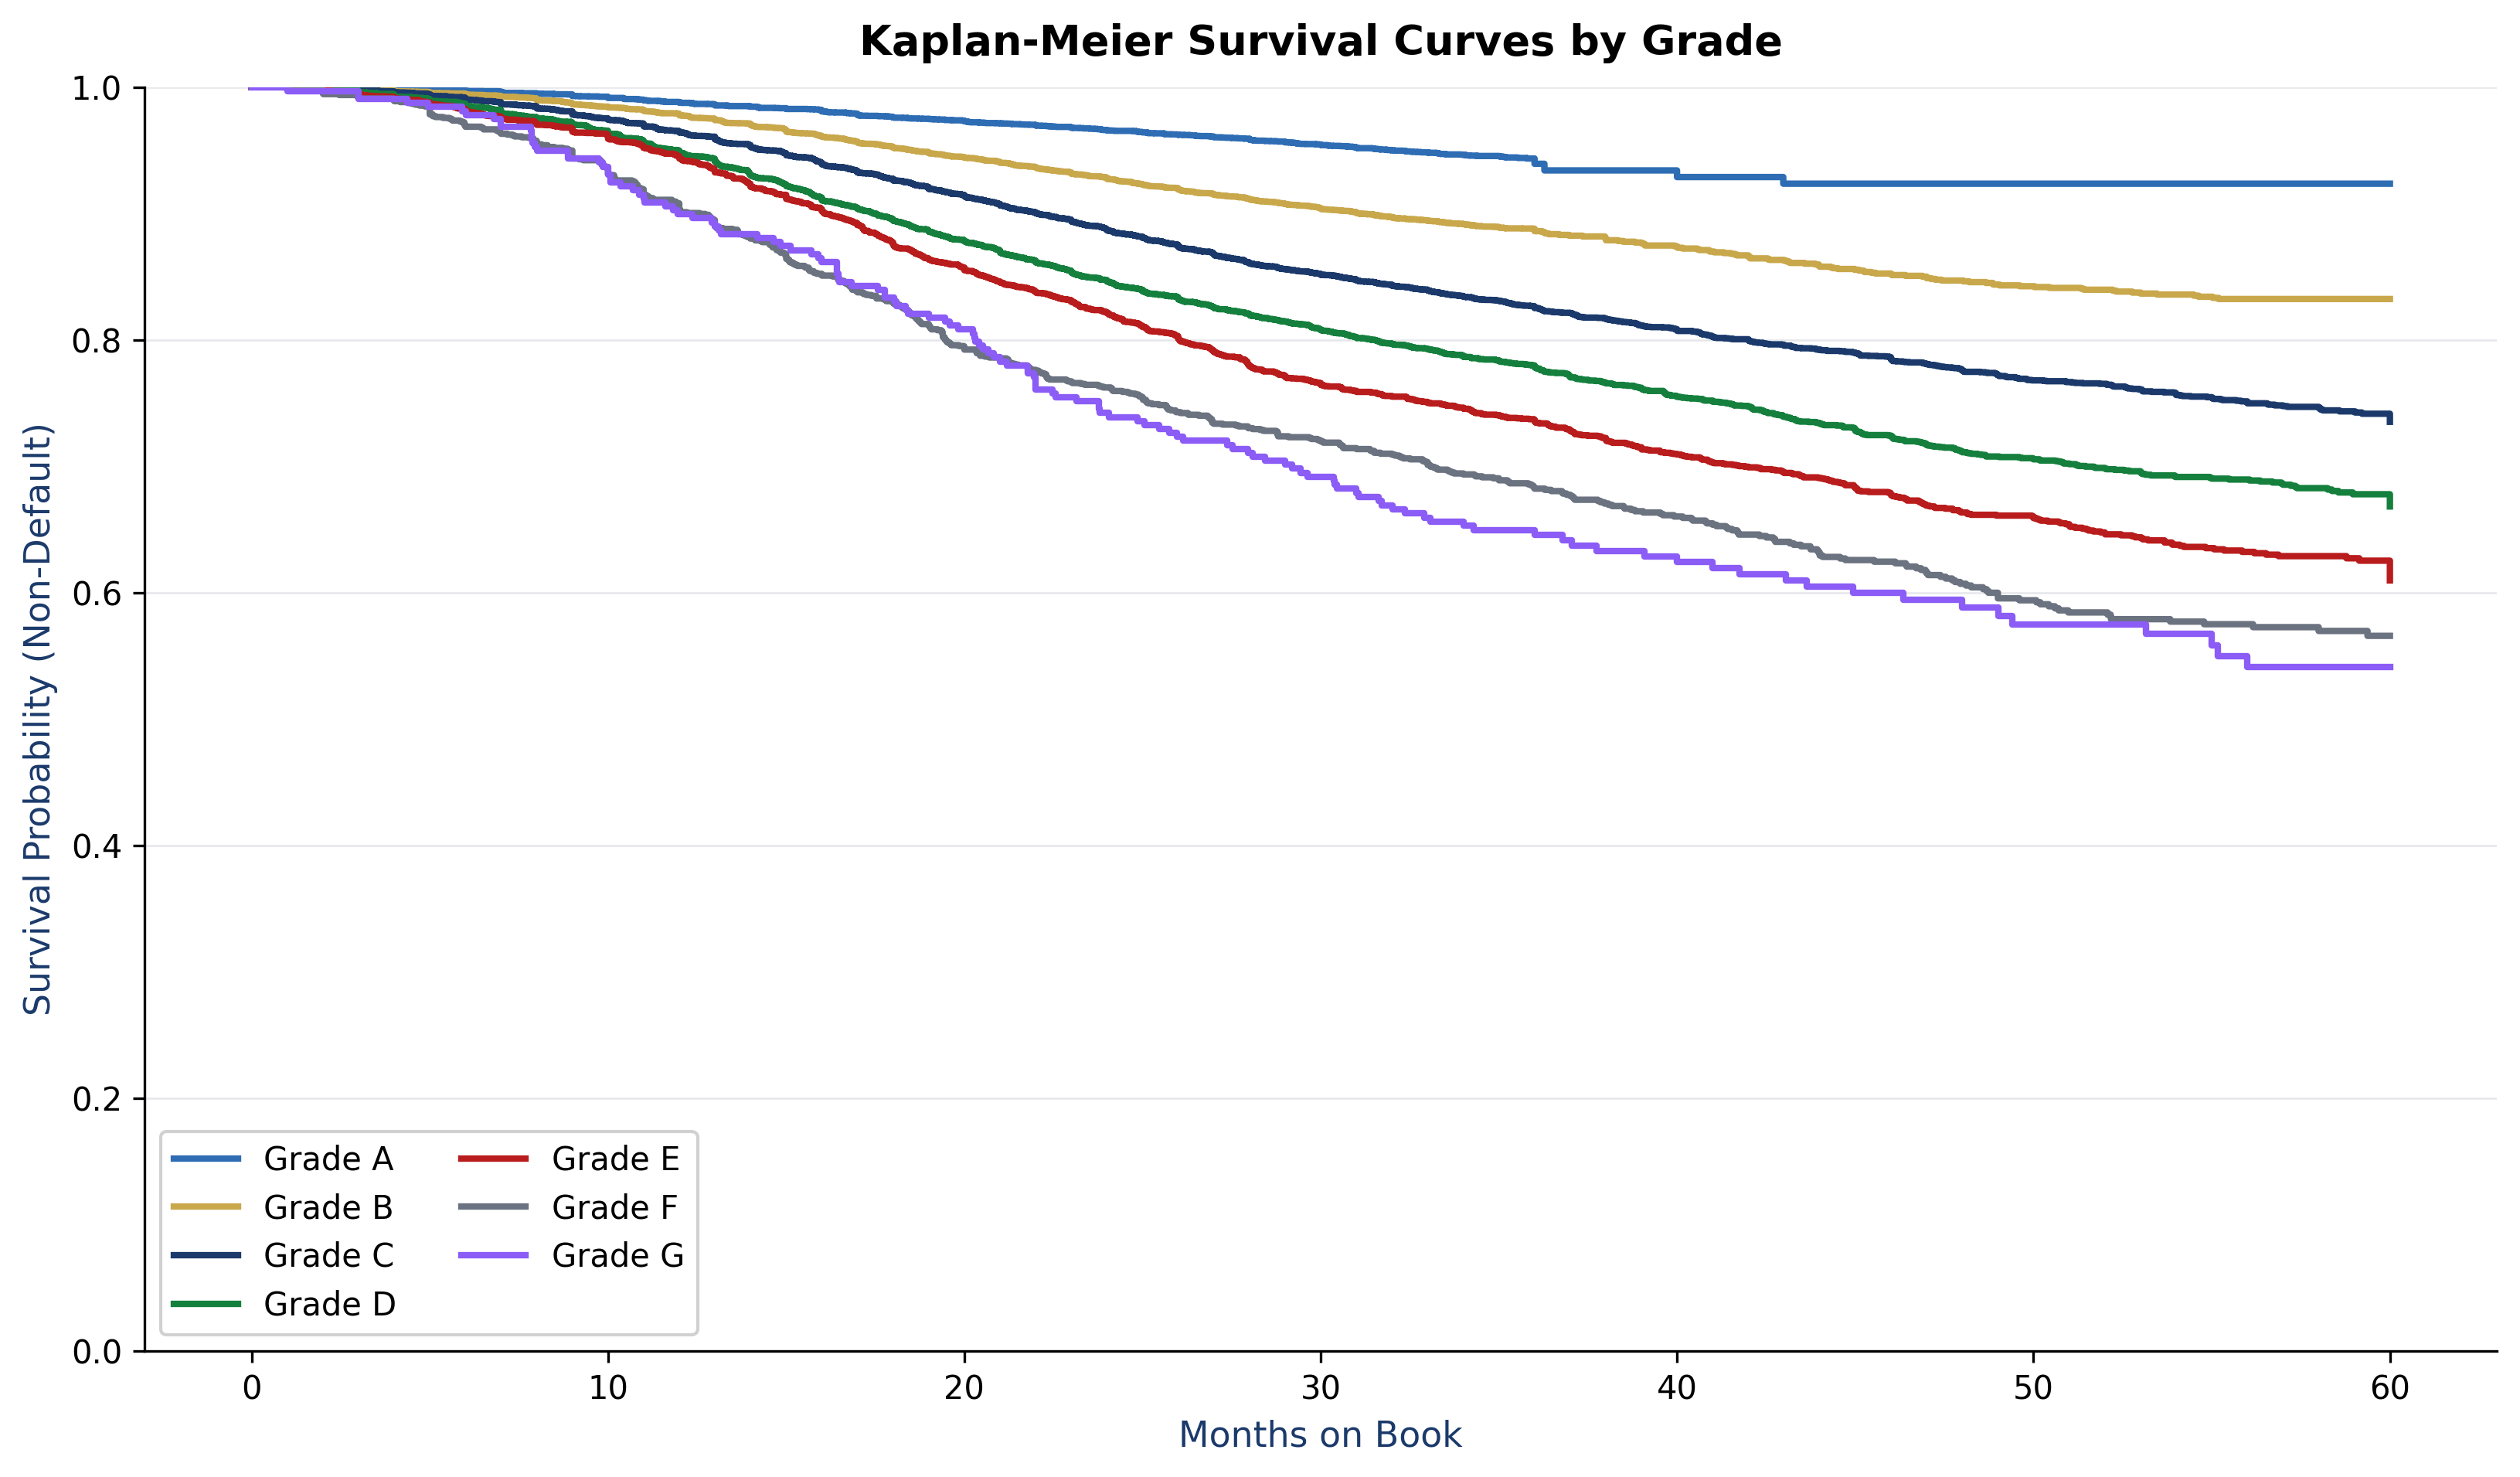
\includegraphics[width=0.66\textwidth]{figures/km_survival_curves.png}
\caption{Kaplan-Meier non-default survival curves by credit grade. Lower grades separate downward, confirming the expected monotone grade--risk ordering.}
\label{fig:km_survival}
\end{figure}

Table~\ref{tab:cox_summary} reports the fitted Cox coefficients, hazard ratios $\exp(\beta)$ and Wald $p$-values. A hazard ratio above $1$ raises the instantaneous default hazard; below $1$ lowers it. The model is fitted on \textbf{standardised} covariates, so each hazard ratio is the effect of a one-standard-deviation move in that covariate and the ratios are directly comparable with each other; the covariate's standard deviation is tabulated alongside so a natural-unit effect can be recovered. This matters because the ridge penalty acts on the raw coefficients: fitted on unstandardised inputs it penalised a covariate measured as a $0.05$--$0.35$ fraction (the interest rate) far more heavily than one measured on a $1$--$7$ integer scale (the grade index), which made the reported multipliers incomparable and shrank the rate effect almost to nothing. On this run the largest per-SD effects attach to credit grade and interest rate, and the smallest to amortisation term (hazard ratio 1.0334 per standard deviation). Each covariate raises the default hazard monotonically as it increases, consistent with the scorecard's risk ordering.

\begin{table}[H]
\centering
\caption{Cox Proportional-Hazards Model --- Covariate Summary (coefficients per standard deviation)}
\label{tab:cox_summary}
\vspace{0.5em}
\begin{tabular}{lrrrr}
\toprule
\textbf{Covariate} & \textbf{SD} & \textbf{Coef ($\beta$ per SD)} & \textbf{Hazard Ratio} & \textbf{$p$-value} \\
\midrule
Credit Grade (A=1..G=7) & 1.317 & +0.16819 & 1.18316 & $<$0.001 \\
Interest Rate & 0.04366 & +0.16578 & 1.18031 & $<$0.001 \\
Debt-to-Income (DTI) & 7.856 & +0.10343 & 1.10897 & $<$0.001 \\
Term (months) & 10.46 & +0.03282 & 1.03336 & $<$0.001 \\
\bottomrule
\end{tabular}
\end{table}

% -----------------------------------------------------------------------------
% 4. LOSS GIVEN DEFAULT (LGD) AND EXPOSURE AT DEFAULT (EAD)
% -----------------------------------------------------------------------------
\section{Loss Given Default (LGD) and Exposure at Default (EAD)}

\subsection{Bimodal Two-Stage LGD Model}
Loss Given Default (LGD) represents the economic loss rate incurred when an exposure defaults. Unlike PD, which models a binary outcome, LGD is continuous, bounded within $[0, 1]$, and heavily bimodal. Defaults typically result in either a complete recovery (LGD = 0, ``cure'') or a near-total loss (LGD close to 1).

To capture this bimodal behavior \parencite{schuermann2004}, a \textbf{two-stage LGD model} is constructed as one of two candidate severity models --- benchmarked against a LightGBM challenger in Section~4.2, with the lower out-of-sample error determining which model is deployed:
\begin{enumerate}
    \item \textbf{Stage 1 (Cure Model):} A gradient-boosted classifier (100 trees, depth 4, learning rate 0.05, class-balanced sample weights) estimates the probability of a zero-loss outcome (cure). Writing $g(\mathbf{x})$ for its fitted cure probability, the loss probability is:
    \begin{equation}
    p_{\text{loss}} = P(\text{LGD} > 0 \mid \text{Default}) = 1 - g(\mathbf{x})
    \end{equation}
    A tree ensemble is used rather than a logistic link because the cure indicator responds non-monotonically to recovery-related covariates; the severity stage below remains a GLM, so the deployed LGD is a hybrid rather than a pure two-stage regression.
    \item \textbf{Stage 2 (Severity Model):} For defaulted loans that incur a loss ($\text{LGD} > 0$), a fractional logit GLM (Binomial family, logit link) models the conditional loss severity \parencite{papke1996,bellotti2012}:
    \begin{equation}
    E[\text{LGD} | \text{LGD} > 0] = \frac{1}{1 + e^{-\mathbf{x}' \boldsymbol{\beta}}}
    \end{equation}
\end{enumerate}
The final predicted LGD is the product of the two stages:
\begin{equation}
\text{LGD}_{\text{pred}} = p_{\text{loss}} \times E[\text{LGD} | \text{LGD} > 0]
\end{equation}

For Basel IRB capital calculations, a \textbf{Downturn LGD} is taken as the 90th percentile of the \emph{realised} severity distribution across loss-incurring defaults (floored at the mean predicted LGD, so the stress can never fall below the central estimate):
\begin{itemize}
    \item \textbf{Mean Expected LGD (deployed model):} 0.8931 (used for IFRS 9 Stage 1 \& 2 provisions)
    \item \textbf{Downturn LGD:} 1.0000 (used for Basel RWA capital calculations)
\end{itemize}

\noindent\textbf{On the magnitude of the downturn uplift.} On this fully unsecured, non-revolving instalment book the realised severity of loss-incurring defaults is concentrated at total loss, so the 90th percentile sits at the cap of the $[0,1]$ range (1.0000), 10.69\,pp above mean LGD. Two consequences follow. It is a real empirical percentile rather than a modelled stress --- more than a tenth of loss-incurring defaults recover nothing at all. And because severity cannot exceed total loss, the Basel capital calculation has no headroom above this figure: any further conservatism must come from PD or EAD, not LGD.

\subsubsection*{Why Mean LGD Is Close to Total Loss}
The realised LGD used to fit and validate the severity model is computed directly from resolved loan outcomes as
\begin{equation}
\text{LGD}_{\text{realised}} = 1 - \frac{\max(0,\ \text{recoveries} - \text{collection\_recovery\_fee})}{\max(1,\ \text{funded\_amnt} - \text{total\_rec\_prncp})}
\end{equation}
i.e.\ net recoveries (gross post-charge-off recoveries less the fee paid to the collection agency) divided by the EAD proxy (funded amount less principal already repaid at charge-off), clipped to $[0,1]$. On this fully unsecured, non-revolving instalment book, post-charge-off cash recoveries are small relative to the outstanding balance, so realised severity concentrates near total loss; the two-stage model's cure probability $p_{\text{loss}}$ separately absorbs the loans that resolve with zero loss, while the conditional severity stage captures how close to total the loss is for the remainder. The published unsecured LGD bands cited below (\textcite{schuermann2004}: 0.45--0.55, corporate/wholesale debt; \textcite{bellotti2012}: 0.25--0.45, revolving retail cards) are measured on portfolios with active collections/settlement programmes and revolving-card structures where partial recoveries are more common; the deployed mean LGD of 0.8931, measured on already-charged-off, non-revolving loans against a book-value EAD proxy with no collateral, is a structurally different (and higher) quantity by construction rather than an anomaly. Its magnitude relative to these bands is discussed further, with numeric verdicts, in the benchmark table (Section~\ref{subsec:benchmarks}).

LGD Benchmark Context: Two severity models are compared on a chronologically held-out selection sample --- a two-stage cure-plus-severity model and a LightGBM challenger --- and the model with the lower error there is deployed for all downstream provisioning and capital; the metrics in Table~\ref{tab:lgd_validation} are then computed on a disjoint reporting sample so the published out-of-sample performance is not measured on the same defaults used for the promotion decision. For unsecured LGD, \textcite{schuermann2004} report a $0.45$--$0.55$ range (a corporate/wholesale-debt review) while \textcite{bellotti2012} document a lower $0.25$--$0.45$ band for revolving retail credit-card portfolios. The deployed mean LGD of 0.8931 and downturn LGD of 1.0000 are assessed against these published ranges in the benchmark table (Section~\ref{subsec:benchmarks}), where any deviation is reported together with its driver. The Downturn LGD is taken at the 90th percentile of the realised severity distribution and used exclusively for Basel IRB capital calculations, providing a buffer of 10.69\,pp above the mean.

\subsection{Out-of-Sample LGD Validation}
The severity model is validated out-of-time on defaulted loans from vintages held out of the fitting window. Table~\ref{tab:lgd_validation} reports the standard LGD backtesting metrics --- Mean Absolute Error (MAE), Root Mean Squared Error (RMSE), the coefficient of determination $R^2$, and a two-sample Kolmogorov-Smirnov (KS) statistic comparing the marginal predicted and realised LGD distributions \parencite{loterman2012benchmarking}. The KS statistic is reported without its $p$-value: at this sample size ($n=$ 74,981) the test is hyper-sensitive to any trivial distributional difference and, being a marginal (not per-loan) comparison, cannot by itself certify calibration; Figure~\ref{fig:lgd_calibration} and the decile table against the $45^{\circ}$ line are the calibration evidence. The aggregate portfolio-level mean LGD sits above the unsecured LGD literature ranges cited in Section~\ref{subsec:benchmarks} (driver discussed there), and the loan-level predictive performance of the deployed severity model is separately weak, with a negative out-of-sample $R^2$ of $-0.0709$ (Table~\ref{tab:lgd_validation}); the rejected two-stage model was materially worse at $R^2 \approx -2.70$, which drove the champion--challenger switch. A negative $R^2$ is a well-documented model risk: realized retail LGD is highly bimodal (concentrated at 0 for cured loans and near 1.0 for write-offs), and predicting the exact loss severity on unsecured, non-collateralized consumer loans is statistically challenging. While the model remains suitable for calculating conservative portfolio-level capital buffers, its loan-level predictions should be treated with caution.

\begin{table}[H]
\centering
\caption{Out-of-Sample LGD Validation Metrics ($n=74,981$ held-out defaults)}
\label{tab:lgd_validation}
\vspace{0.5em}
\begin{tabular}{lr}
\toprule
\textbf{Metric} & \textbf{Value} \\
\midrule
Mean Absolute Error (MAE) & 0.0763 \\
Root Mean Squared Error (RMSE) & 0.1080 \\
Coefficient of Determination ($R^2$) & -0.0709 \\
KS Statistic (marginal dist., pred vs actual) & 0.5490 \\
\bottomrule
\end{tabular}
\end{table}

\begin{figure}[H]
\centering
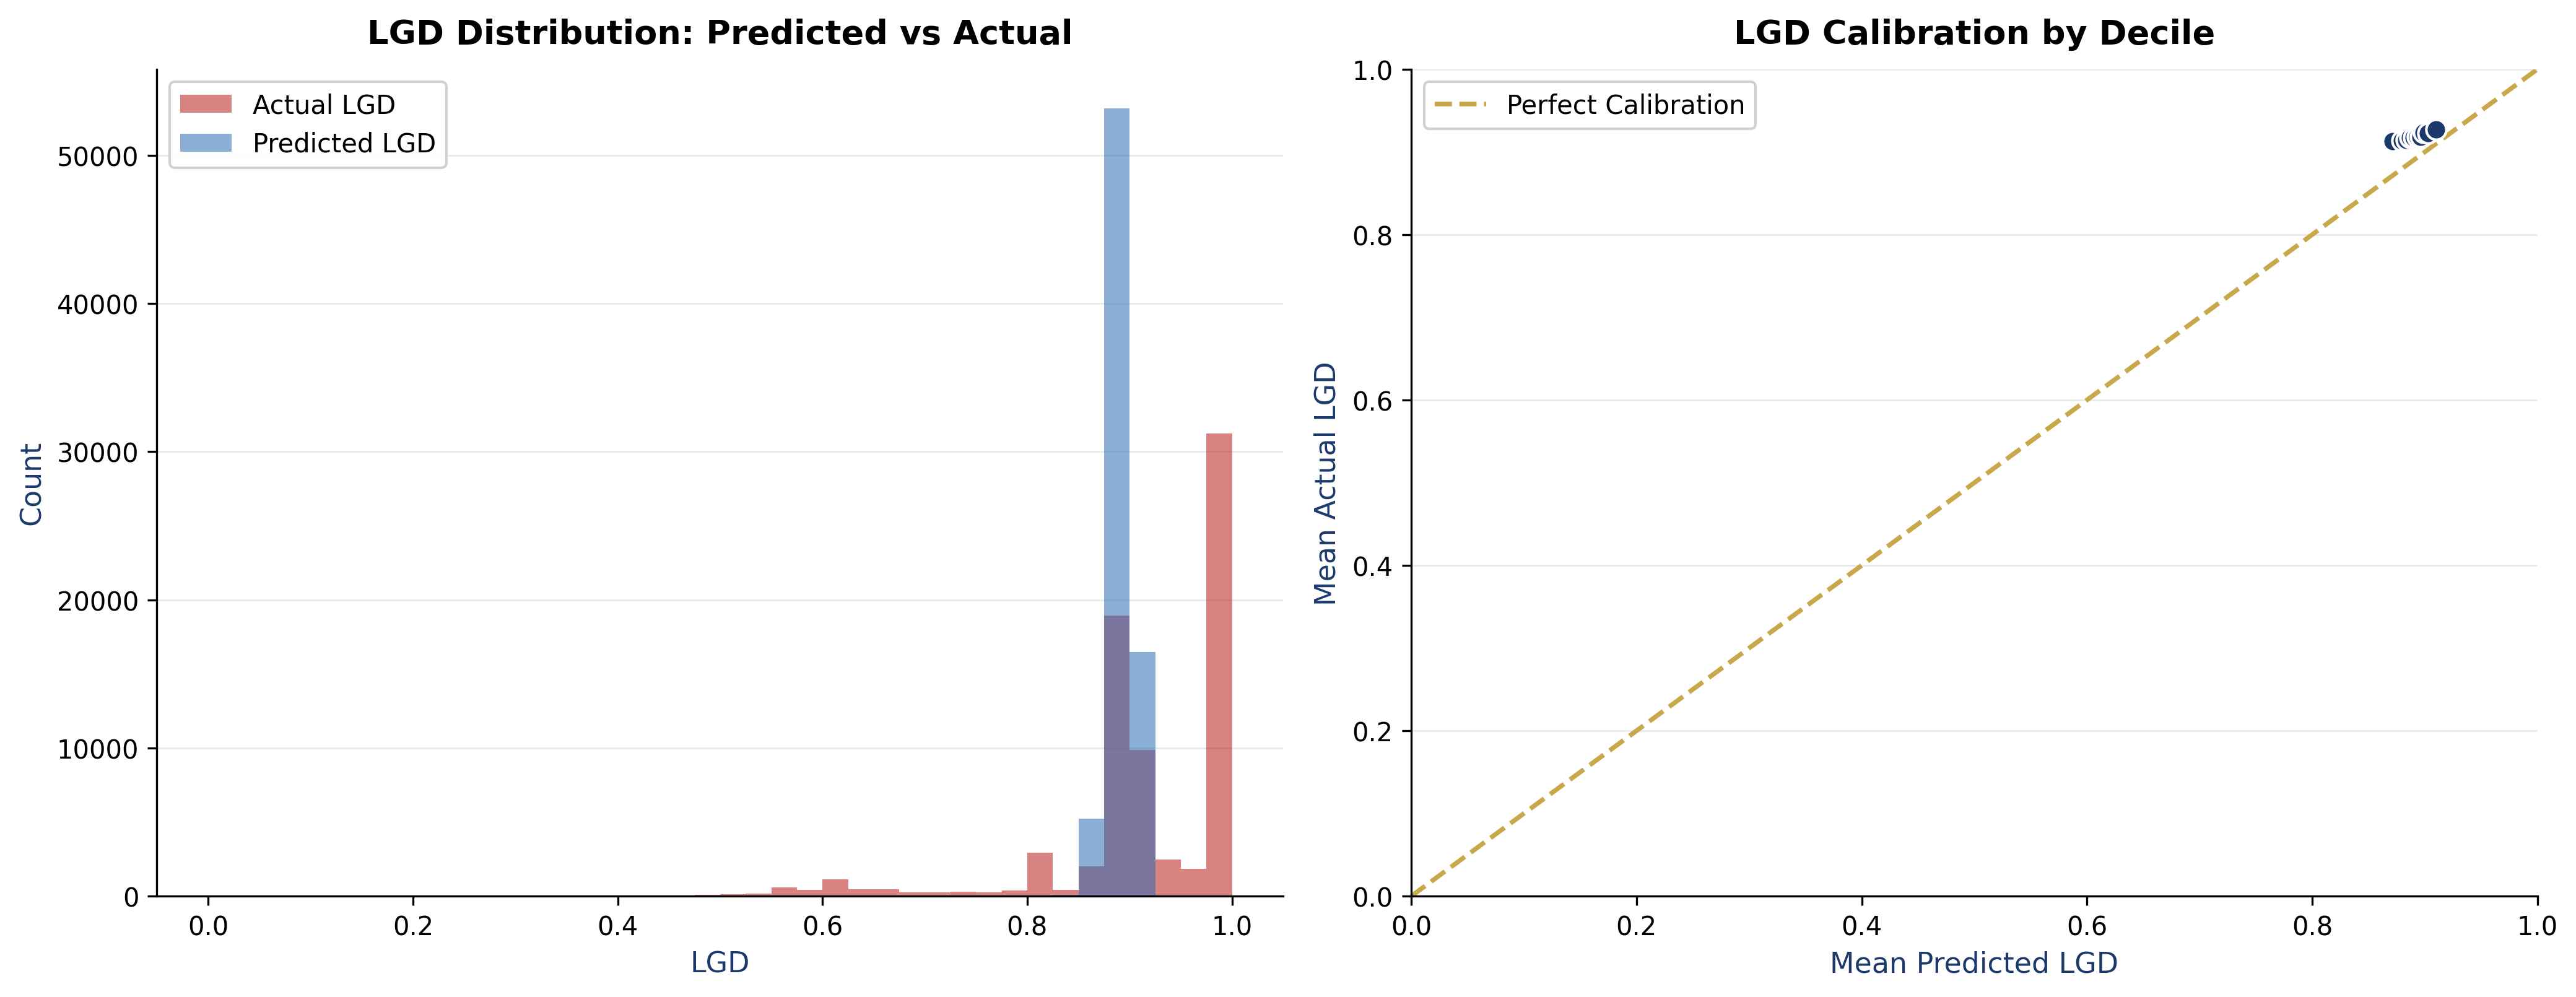
\includegraphics[width=\textwidth]{figures/validation/lgd_calibration.png}
\caption{LGD validation: (left) predicted vs realised LGD distributions; (right) mean realised vs mean predicted LGD by predicted decile against perfect calibration.}
\label{fig:lgd_calibration}
\end{figure}

\subsection{Amortisation-Based EAD for Term Loans}
Exposure at Default (EAD) represents the outstanding gross balance owed by the borrower at the moment of default. For fully-drawn, non-revolving consumer installment loans, the outstanding principal amortizes deterministically over time. EAD is modeled using a closed-form annuity amortization formula:
\begin{equation}
EAD(t) = \text{funded\_amnt} \times \frac{1 - (1 + r)^{-(T - t)}}{1 - (1 + r)^{-T}}
\end{equation}
where $r$ is the monthly interest rate on the loan contract, $T$ is the original term in months, and $t$ is the elapsed Months-on-Book (MOB) at default.

For revolving credit facilities (such as credit cards or overdraft limits), EAD must capture future drawdowns using a Credit Conversion Factor (CCF):
\begin{equation}
EAD = \text{Drawn Balance} + \text{CCF} \times \text{Undrawn Limit}
\end{equation}
Since Lending Club loans are fully drawn installment loans with no revolving limits, the undrawn limit is zero. Using the closed-form amortization formula to calculate outstanding principal is an appropriate simplification, which is fully documented and standard in retail banking.

% -----------------------------------------------------------------------------
% 5. BASEL IRB REGULATORY CAPITAL \& CAPITAL STRESS TESTING
% -----------------------------------------------------------------------------
\section{Basel IRB Capital \& Capital Stress Testing}

Throughout this report, $Z < 0$ corresponds to an adverse macroeconomic shock (recession); $Z > 0$ corresponds to a favourable shock (expansion). This sign convention applies uniformly to the Vasicek stress test below, the IFRS~9 macro-scenario mapping (Table~\ref{tab:macro_regression}), and the ECL sensitivity analysis (Figure~\ref{fig:ecl_tornado}).

\subsection{ASRF Vasicek Model and the ``Other Retail'' Formula}
Under the Basel II/III framework \parencite{bcbs2004}, banks calculate capital requirements for retail exposures using the Asymptotic Single Risk Factor (ASRF) model \parencite{vasicek2002}. This framework assumes that portfolio risk is driven by a single systematic macroeconomic factor. The retail supervisory correlation ($R$) and capital requirement ($K$) formulas for the ``Other Retail'' asset class are:
\begin{equation}
R = 0.03 \times \frac{1 - e^{-35 \times PD}}{1 - e^{-35}} + 0.16 \times \left[ 1 - \frac{1 - e^{-35 \times PD}}{1 - e^{-35}} \right]
\end{equation}
\begin{equation}
K = \text{Downturn LGD} \times \Phi\!\left( \frac{\Phi^{-1}(PD) + \sqrt{R}\,\Phi^{-1}(0.999)}{\sqrt{1 - R}} \right) - PD \times \text{Downturn LGD}
\end{equation}
\parencite[§328]{bcbs2004}. Where $\Phi$ is the standard normal cumulative distribution function, $\Phi^{-1}$ is the inverse standard normal CDF, and the confidence level is set to \textbf{99.9\%}. Risk-Weighted Assets (RWA) are calculated by scaling the capital requirement ($K$):
\begin{equation}
RWA = K \times 12.5 \times EAD
\end{equation}

\textbf{PD horizon.} The $PD$ entering this formula is a \textbf{one-year} probability of default, as \S328 requires. The scorecard's own target is the loan's terminal resolved status, so its direct output is a \emph{lifetime} PD; it is converted at the point of use under a constant marginal-hazard assumption over the remaining term,
\begin{equation}
PD_{\text{12m}} = 1 - (1 - PD_{\text{lifetime}})^{12/T},
\end{equation}
with $T$ the contractual term in months. On this portfolio that is a mean of 20.96\% lifetime against 6.64\% over twelve months. The same one-year measure drives the Expected Loss of Section~5.2, the per-annum profit and RAROC calculation of Section~9, and the stress test below; the lifetime figure is retained where its horizon is the correct one, namely IFRS~9 staging and lifetime ECL. Substituting the lifetime PD into a one-year capital formula --- as an earlier version of this engine did --- inflates RWA density and, because $K$ is concave in $PD$, can make stressed RWA fall below base RWA.

\subsection{Basel IRB Capital vs.\ Standardised Approach (SA) Reference}
Table~\ref{tab:basel_comparison} compares the capital requirements calculated using the Internal Ratings-Based (IRB) approach against the Standardized Approach (SA) reference (75\% risk weight):

\begin{table}[H]
\centering
\caption{Basel IRB Regulatory Capital Comparison against Standardised Approach}
\label{tab:basel_comparison}
\vspace{0.5em}
\begin{tabular}{p{5.0cm}cc}
\toprule
\textbf{Capital Metric} & \textbf{Basel IRB (Risk-Sensitive)} & \textbf{Standardised Approach (SA)} \\
\midrule
Total Portfolio RWA & \$6,031,656,591 & \$2,797,336,487 \\
Minimum Capital Reserve (8\%) & \$482,532,527 & \$223,786,919 \\
Portfolio RWA Density & 161.7\% & 75.0\% \\
\bottomrule
\end{tabular}
\end{table}

The risk-sensitive IRB approach determines an RWA density of \textbf{161.7\%}. This risk-sensitive capital requirement demonstrates the value of developing internal risk models, indicating a necessary capital surcharge of \textbf{\$258,745,608} compared to the flat Standardised Approach, ensuring that the bank remains adequately capitalised against default stress in this retail portfolio.

\subsection{Basel III Economic Capital \& Macro Stress Testing}
We implemented a mathematically rigorous \textbf{Vasicek credit cycle stress test} \parencite{engelmann2011} to measure how the portfolio's expected and unexpected losses respond to a severe systematic contraction:
\begin{equation}
PD_{\text{PiT}}(Z) = \Phi\left( \frac{\Phi^{-1}(PD_{\text{TTC}}) - \sqrt{\rho} Z}{\sqrt{1 - \rho}} \right)
\end{equation}
where the systematic risk factor is set to an extreme stress level of $Z = -2.0$ (representing a severe economic recession with a 2.28\% probability of occurrence) under an asset correlation of $\rho = 0.15$.

Table~\ref{tab:stress_testing} compares the portfolio's capital adequacy reserves under standard conditions against the severe Vasicek macroeconomic stress state:

\begin{table}[h]
    \centering
    \caption{Basel IRB Economic Capital Stress Test (Z=-2.0 vs TTC)}
    \label{tab:stress_testing}
    \vspace{0.5em}
    \begin{tabular}{lrrr}
        \toprule
        \textbf{Dimension} & \textbf{Base IRB} & \textbf{Stressed IRB} & \textbf{Increase} \\
        \midrule
        \textbf{Expected Loss (EL)} & \$279,373,219 & \$819,553,574 & 193.4\% \\
        \textbf{Risk-Weighted Assets (RWA)} & \$6,031,656,591 & \$8,598,289,561 & 42.6\% \\
        \textbf{Capital Requirement (8\%)} & \$482,532,527 & \$687,863,165 & 42.6\% \\
        \bottomrule
    \end{tabular}
\end{table}

Under the severe systematic stress shock ($Z = -2.0$), the portfolio's expected loss rises by 193.4\%, and the RWA expands by 42.6\%. This result feeds directly into capital adequacy planning (ICAAP).

\subsection{Monte Carlo Economic Capital: VaR and Expected Shortfall}
Basel IRB delivers \emph{regulatory} capital under a closed-form, infinitely-granular single-factor assumption. \emph{Economic} capital is read directly off the full simulated portfolio loss distribution, which captures the tail more faithfully and distinguishes Value-at-Risk (VaR) from Expected Shortfall (ES / CVaR), the coherent tail measure now favoured under the Basel FRTB framework \parencite{mcneil2015}. We simulate the loss distribution with a Monte Carlo ASRF (Vasicek) engine: a single systematic factor $Z \sim N(0,1)$ is drawn per scenario, obligors' conditional PDs follow Equation~(\ref{eq:vasicek_ec}), and idiosyncratic default risk enters through a per-bucket Binomial draw.
\begin{equation}
\label{eq:vasicek_ec}
p_i(Z) = \Phi\!\left( \frac{\Phi^{-1}(PD_i) - \sqrt{\rho}\,Z}{\sqrt{1 - \rho}} \right), \qquad
L = \sum_i \mathbb{1}\{\text{default}_i\} \cdot LGD_i \cdot EAD_i .
\end{equation}

\begin{figure}[H]
\centering
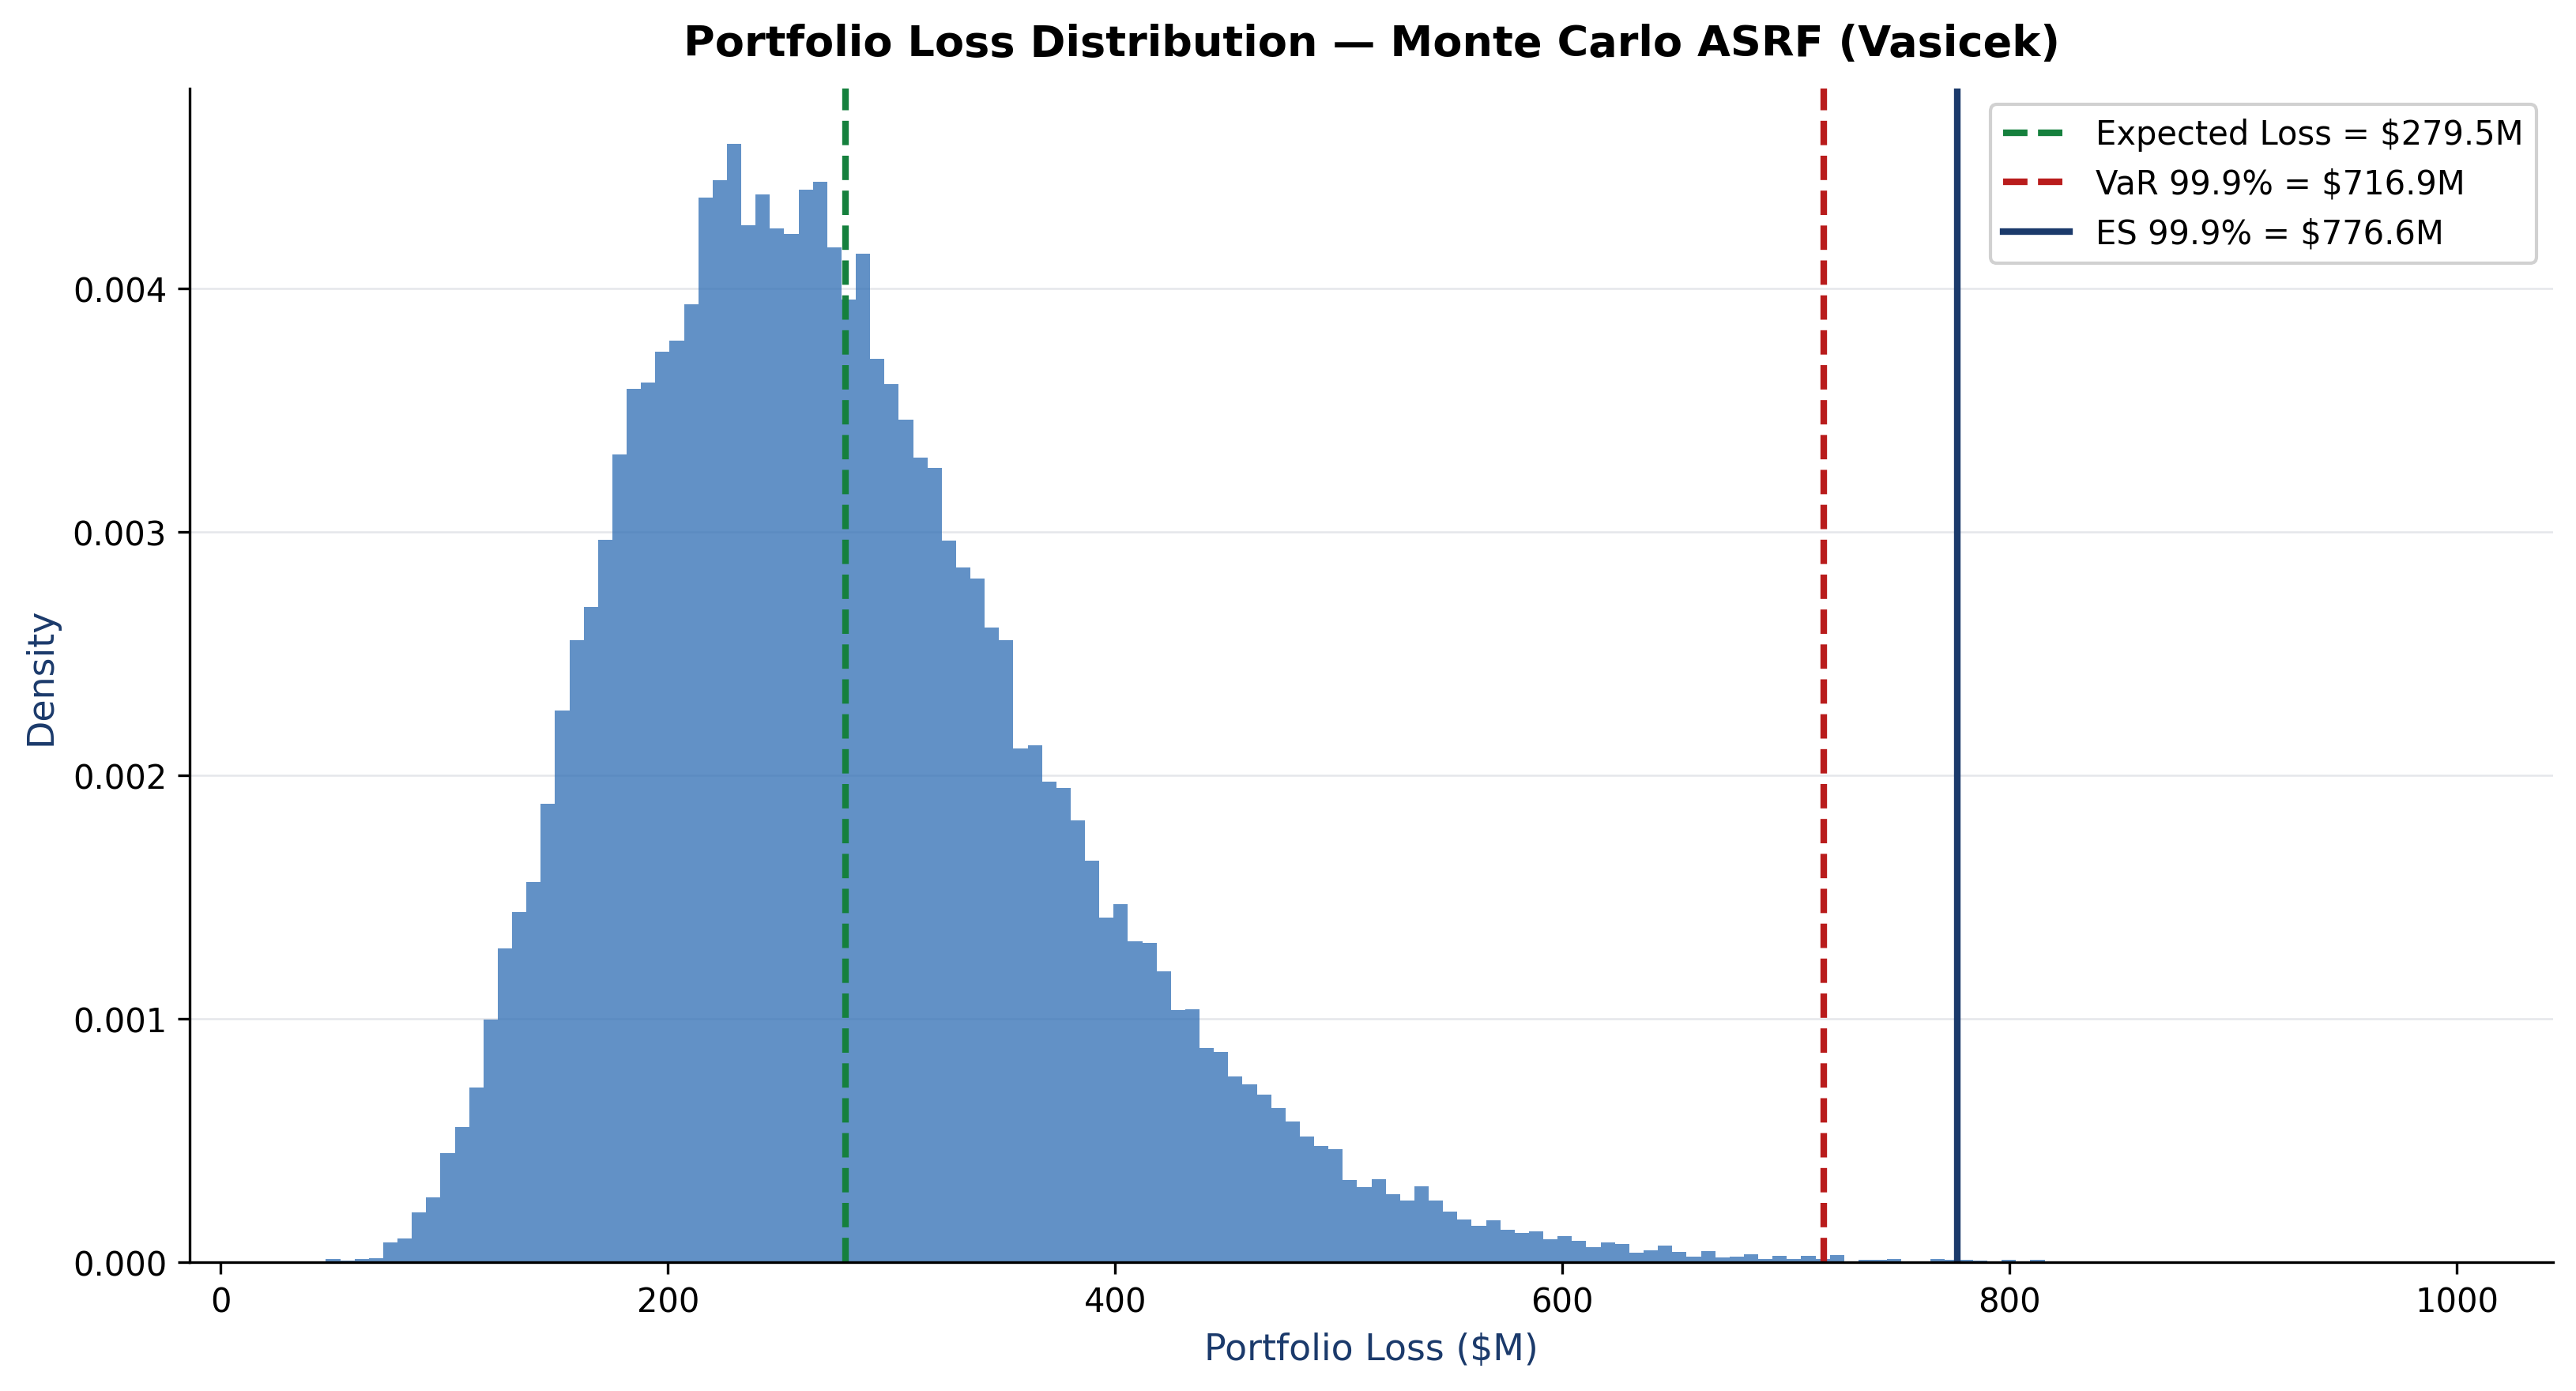
\includegraphics[width=0.66\textwidth]{figures/loss_distribution.png}
\caption{Monte Carlo portfolio loss distribution under the ASRF single-factor model, with Expected Loss, VaR and Expected Shortfall marked.}
\label{fig:loss_distribution}
\end{figure}

Table~\ref{tab:risk_measures} reports the resulting risk measures. Expected Shortfall exceeds VaR by construction ($ES \geq VaR \geq EL$), and the ES-based economic capital buffer is compared against the Basel IRB regulatory capital requirement.

The simulation uses the \emph{same} supervisory ``Other Retail'' correlation curve as the IRB calculation it is compared against, evaluated per PD bucket. This matters for interpretation: a flat $\rho = 0.15$ against a supervisory $R$ that collapses toward $0.03$ at this book's PD levels would make the EC-to-regulatory-capital ratio largely an artefact of a five-fold correlation difference rather than the tail fidelity it is meant to demonstrate. As a disclosed sensitivity, holding $\rho$ flat at 0.15 instead gives economic capital of \$1.22bn (253.4\% of regulatory capital). The 99.9\% quantile rests on 50 tail draws, giving a Monte Carlo standard error of \$8.3m on VaR; the figures should be read at that precision, not to the cent.

\begin{table}[H]
\centering
\caption{Monte Carlo Economic Capital --- Risk Measures (ASRF, $N=50,000$ simulations, supervisory $R(\mathrm{PD}) \in [0.03, 0.16]$)}
\label{tab:risk_measures}
\vspace{0.5em}
\begin{tabular}{lr}
\toprule
\textbf{Risk Measure} & \textbf{Value (\$M)} \\
\midrule
Expected Loss (EL) & 279.49 \\
Value-at-Risk (VaR 99.9\%) & 716.95 \\
Expected Shortfall (ES 99.9\%) & 776.59 \\
Unexpected Loss (UL $=$ VaR $-$ EL) & 437.46 \\
\midrule
\textbf{Economic Capital (EC $=$ ES $-$ EL)} & \textbf{497.10} \\
Basel IRB Regulatory Capital (8\%) & 482.53 \\
EC / Regulatory Capital & 103.0\% \\
\bottomrule
\end{tabular}
\end{table}

\subsection{Concentration Risk: HHI and Granularity Adjustment}
The Basel ASRF model assumes an infinitely-granular, perfectly-diversified portfolio; residual name and segment concentration therefore requires a capital add-on. We measure concentration with the Herfindahl-Hirschman Index (HHI) across exposure dimensions --- credit grade, loan purpose and borrower state --- reporting the effective number of equal-sized exposures $1/\text{HHI}$ for each (Table~\ref{tab:hhi}). Figure~\ref{fig:concentration} visualises the exposure distribution per dimension. The residual single-name concentration is capitalised through a simplified Gordy-Lutkebohmert granularity adjustment, an additive surcharge above the ASRF regulatory capital.

\begin{table}[H]
\centering
\caption{Portfolio Concentration --- Herfindahl-Hirschman Index by Dimension}
\label{tab:hhi}
\vspace{0.5em}
\begin{tabular}{lrrrr}
\toprule
\textbf{Dimension} & \textbf{HHI} & \textbf{Eff. $N$} & \textbf{Categories} & \textbf{Top Share} \\
\midrule
Credit Grade & 0.2129 & 4.7 & 7 & 28.6\% \\
Loan Purpose & 0.4275 & 2.3 & 14 & 61.2\% \\
Borrower State & 0.0549 & 18.2 & 51 & 15.0\% \\
\midrule
\multicolumn{5}{l}{\textbf{Granularity Adjustment (capital surcharge):} \$407} \\
\midrule
\multicolumn{5}{p{0.95\linewidth}}{\footnotesize The Gordy--L\"utkebohmert granularity adjustment is a single-\emph{name} idiosyncratic-risk add-on ($\sum_i \mathrm{UL}_i^2 / 2\,\mathrm{EAD}_{\text{tot}}$); on this loan-granular book (hundreds of thousands of small exposures) it is near-zero by construction and is distinct from the segment-level HHI figures above, which measure concentration across grade / purpose / state buckets rather than individual names.} \\
\bottomrule
\end{tabular}
\end{table}

\begin{figure}[H]
\centering
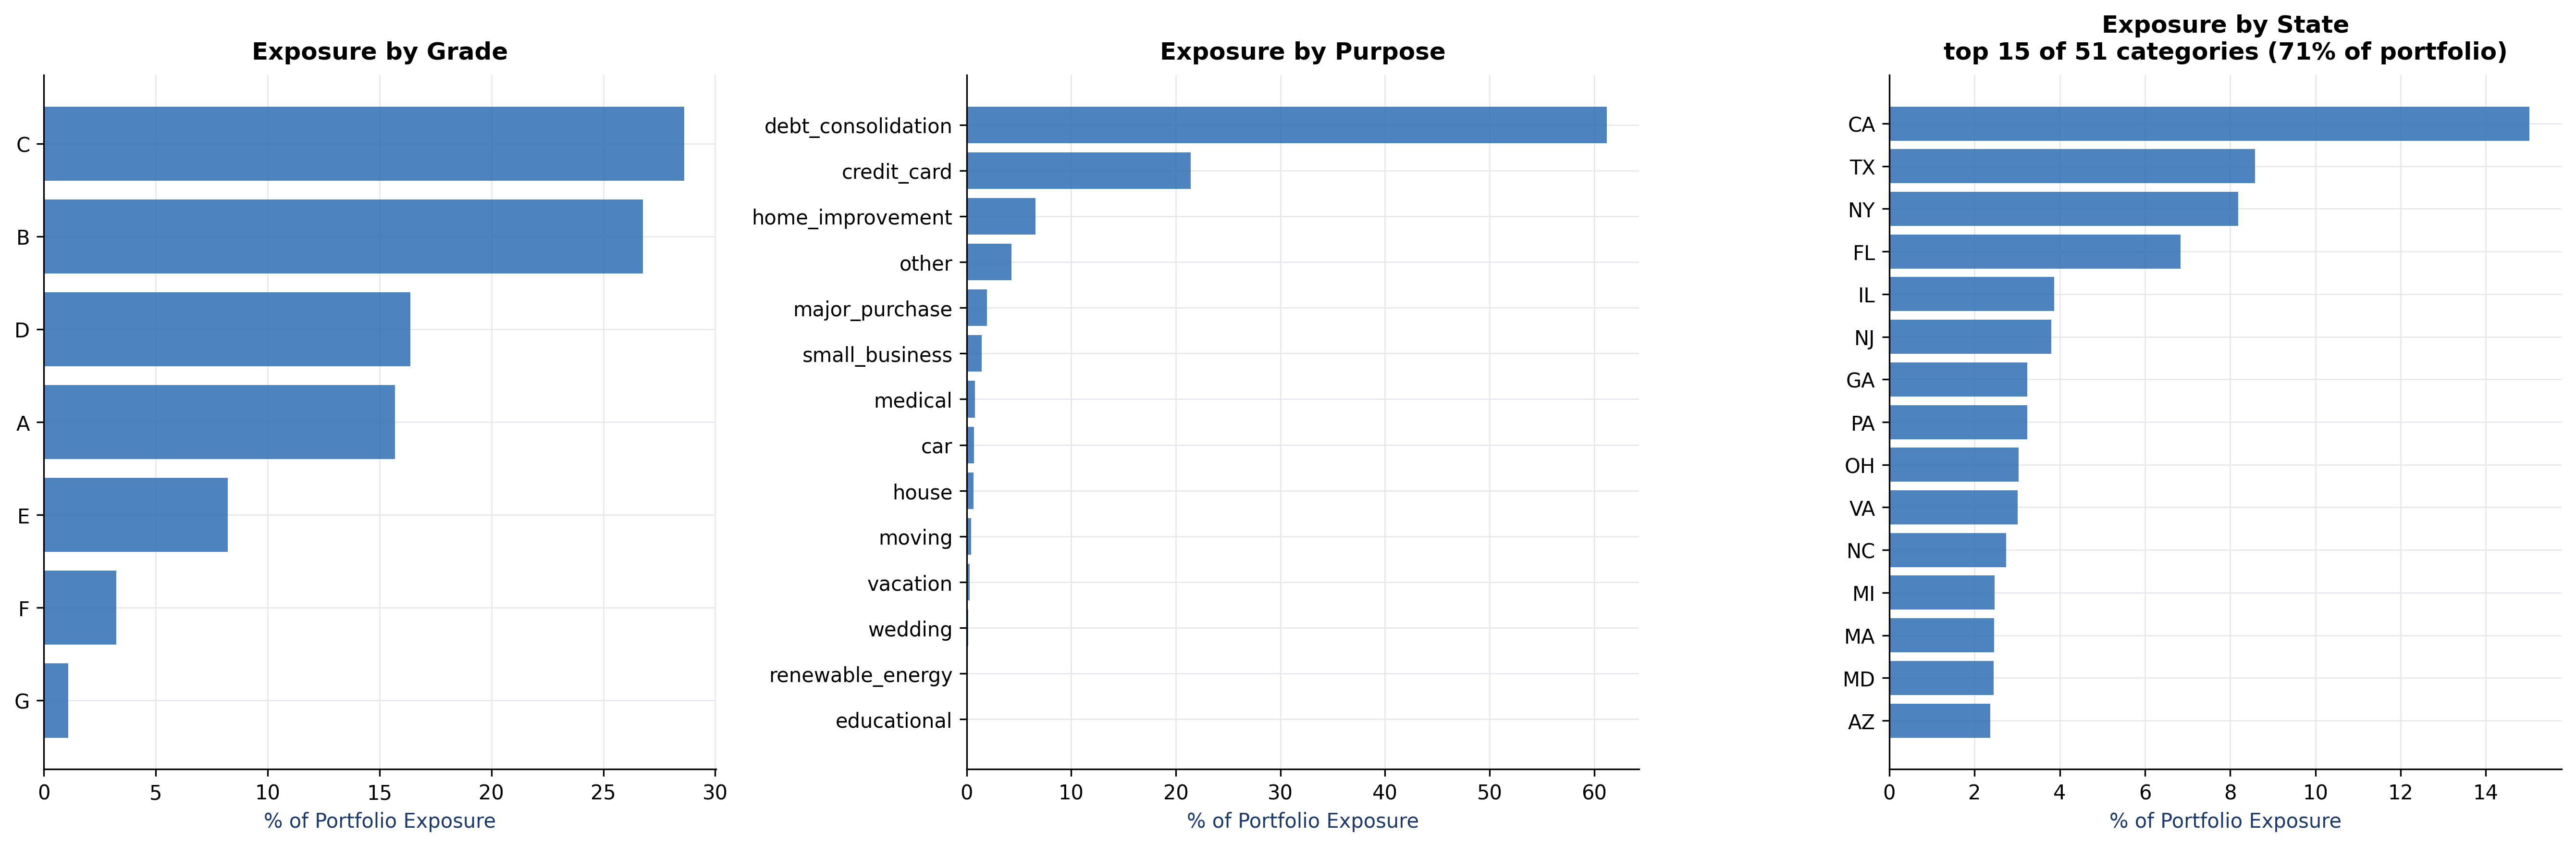
\includegraphics[width=\textwidth]{figures/concentration_risk.png}
\caption{Portfolio exposure concentration by credit grade, loan purpose and borrower state (top 15).}
\label{fig:concentration}
\end{figure}

% -----------------------------------------------------------------------------
% 6. IFRS 9 EXPECTED CREDIT LOSS (ECL) ENGINE
% -----------------------------------------------------------------------------
\section{IFRS 9 Expected Credit Loss (ECL) Engine}

\subsection{Three-Stage Staging and Significant Increase in Credit Risk (SICR)}
IFRS~9 \parencite{iasb2014} introduces a forward-looking impairment model based on three credit quality stages:
\begin{itemize}
    \item \textbf{Stage 1 (Performing):} No Significant Increase in Credit Risk (SICR) since origination. ECL is measured over a \textbf{12-month horizon}.
    \item \textbf{Stage 2 (Underperforming):} SICR is detected since origination, but the loan is not defaulted. ECL is measured over the \textbf{remaining lifetime} of the loan.
    \item \textbf{Stage 3 (Credit-Impaired):} Non-performing loans. ECL is measured over the \textbf{remaining lifetime}, with PD set to \textbf{100\%}. \emph{Implementation note:} the dataset carries no monthly days-past-due panel, so Stage~3 is not identified by a 90+ DPD observation but by the loan's terminal resolved status (the modelling target). This makes the Stage~3 population a hindsight classification --- see Section~10, where its effect on the headline ECL is quantified.
\end{itemize}

Staging is evaluated under the \textbf{baseline} scenario ($Z = -0.1915$), the same central expectation the provision is anchored to. It was previously computed at $Z = 0$, which corresponds to none of the three priced scenarios: the Vasicek conditional-PD function does not return the unconditional PD at $Z = 0$, so loans were being sorted into stages under macroeconomic conditions that appeared nowhere else in the calculation.

A Significant Increase in Credit Risk (SICR) \parencite{novotny2016} is triggered if:
\begin{itemize}
    \item The ratio of lifetime PD to origination PD exceeds \textbf{2.5$\times$}.
    \item The absolute lifetime PD exceeds \textbf{20\%}.
    \item A delinquency backstop fires. The IFRS~9 standard backstop is 30+ days past due at the reporting date; absent a DPD panel, the implemented proxy is \texttt{delinq\_2yrs} $\geq 1$, i.e.\ at least one delinquency recorded in the two years \emph{before} origination. This is an application-time credit-history flag rather than a current-delinquency measure, and is a documented deviation from the standard (Section~10).
\end{itemize}

\subsection{PD Term Structure and Lifetime Expected Credit Loss}
Rather than using static 12-month PDs, the IFRS~9 engine models the lifetime PD curve using a discrete hazard model \parencite[Ch.~7]{lando2004}. The survival probability ($S(t)$) and marginal monthly PD ($m(t)$) are calculated as:
\begin{equation}
S(t) = \prod_{s=1}^{t} (1 - h(s)), \quad m(t) = S(t-1) \times h(t)
\end{equation}
where $h(t)$ is the conditional default hazard at month $t$. The final ECL is the discounted sum of expected losses over the relevant horizon ($H$):
\begin{equation}
ECL = \sum_{t=1}^{H} \frac{m(t) \times \text{LGD}(t) \times \text{EAD}(t)}{(1 + \text{EIR})^t}
\end{equation}
\parencite{bellini2019}. Where $\text{EIR}$ is the Effective Interest Rate derived from the loan's contractual pricing. \emph{Implementation note:} in the current engine $\text{LGD}(t)$ and $\text{EAD}(t)$ are held constant at their per-loan point estimates across the summation --- exposure is evaluated once (Section~4.3) rather than re-amortised month by month --- so the formula above is the general statement and the implementation is its constant-exposure special case. This is conservative for amortising loans, since the outstanding balance in fact declines over the horizon.

\subsubsection*{Lifetime PD Calibration: Validating the ECL-Driving Term Structure}
The lifetime PD $1 - S(H)$ used directly in the equation above is produced by the discrete hazard model and enters the ECL sum unchanged. It is a distinct estimator from the scorecard's 12-month PD and is \emph{not} passed through the scorecard's out-of-sample isotonic/Platt recalibration described in Section~7.2 --- that recalibration only touches the 12-month PD used for expected loss, Basel RWA, and SICR-origination staging. Rather than silently trusting an unvalidated PD inside the loss-driving formula, Table~\ref{tab:lifetime_pd_calibration} instead validates the hazard model's own lifetime PD against realised lifetime default rates by origination vintage (restricted to vintages originated in or before 2016, since 2017--2018 charge-offs are not yet resolved in the 2018Q4 snapshot; note the 2016 cohort itself is only partially matured, so its observed rate is still right-censored). A ratio near 1.0 indicates the hazard PD entering the ECL sum is itself reasonably calibrated to realised outcomes; a ratio materially outside the $[0.5, 1.5]$ tolerance band would indicate that the term structure --- not just the 12-month scorecard PD --- requires recalibration before it can be trusted in the ECL sum, a finding this report would then surface explicitly rather than let pass silently into the headline coverage ratio.

\begin{table}[H]
\centering
\caption{Hazard Model Lifetime PD vs Realised Lifetime Default Rate (Matured Vintages)}
\label{tab:lifetime_pd_calibration}
\vspace{0.5em}
\begin{tabular}{lrrrr}
\toprule
\textbf{Vintage} & \textbf{N} & \textbf{Predicted Lifetime PD} & \textbf{Observed Default Rate} & \textbf{Ratio} \\
\midrule
2007 & 603 & 13.88\% & 26.20\% & 0.53 \\
2008 & 2,393 & 13.74\% & 20.73\% & 0.66 \\
2009 & 5,281 & 12.42\% & 13.69\% & 0.91 \\
2010 & 12,537 & 14.46\% & 14.01\% & 1.03 \\
2011 & 21,721 & 15.74\% & 15.18\% & 1.04 \\
2012 & 53,367 & 16.56\% & 16.20\% & 1.02 \\
2013 & 134,807 & 18.64\% & 15.60\% & 1.19 \\
2014 & 223,437 & 18.23\% & 18.57\% & 0.98 \\
2016 & 297,651 & 17.54\% & 24.46\% & 0.72 \\
\midrule
\textbf{All mature vintages} & 751,797 & 17.72\% & 20.00\% & \textbf{0.89} \\
\bottomrule
\multicolumn{5}{p{0.95\linewidth}}{\footnotesize $\dagger$ outside the $[0.5, 1.5]$ tolerance band. Restricted to vintages originated in or before 2016: the 2018Q4 snapshot has not yet resolved recoveries/charge-offs for 2017--2018 originations, so their observed default status is right-censored. The 2015 cohort is absent because it falls in the excluded train/OOT grey zone (Section~2.3); the 2016 cohort is included but is itself only partially matured, which depresses its ratio.} \\
\end{tabular}
\end{table}

\subsection{Forward-Looking Macroeconomic Scenarios}
To ensure ECL provisions are forward-looking and compliant with IFRS 9, we implement an Ordinary Least Squares (OLS) macroeconomic regression with imposed economic sign priors, supported by the ADF, Granger-causality and Johansen time-series diagnostics reported in Section~6.3. This framework dynamically links quarterly historical default rates of the LendingClub portfolio to key US macroeconomic indicators, sourced live from the official FRED (St.\ Louis Fed) API: the Unemployment Rate (UNRATE), real GDP growth (GDP\_growth, from GDPC1 --- \emph{real}, not nominal, so that inflation does not enter the regression twice alongside CPI), the Federal Funds Rate (FEDFUNDS), CPI Inflation (CPI\_inflation), and House Price Index Growth (HPI\_growth, from the seasonally-adjusted Case-Shiller US National HPI), a collateral-value indicator via which rising home prices support household wealth and reduce default risk.

The OLS model determines the sensitivity (elasticity) of the portfolio default rate to each economic factor. These sensitivities are used to predict default rates under three standardized economic scenarios (Baseline, Upside, and Downside). The macro-predicted default rates are then mathematically mapped to systematic credit cycle shocks (Vasicek $Z$-shocks) using the supervisory retail correlation parameter ($\rho = 0.15$):
\begin{equation}
Z_{\text{shock}} = \frac{\Phi^{-1}(\text{TTC\_DR}) - \Phi^{-1}(\text{PIT\_DR}) \times \sqrt{1 - \rho}}{\sqrt{\rho}}
\end{equation}
where $\text{TTC\_DR}$ is the long-run average (Through-the-Cycle) default rate, and $\text{PIT\_DR}$ is the Point-in-Time default rate predicted under each macroeconomic scenario.

\textbf{The shock is applied once, at the horizon on which it was calibrated.} $\text{TTC\_DR}$ is the share of loans that default at any point in their life, so $Z$ describes a \emph{lifetime} quantity. Applying that same Vasicek transform to each \emph{monthly} hazard would compound it over the whole term, lifting cumulative PD far past the ratio the scenario actually targets. Instead the shock is applied once, to each loan's cumulative default probability over its own term, and the resulting uplift is redistributed across months as a proportional-hazards scaling: with $S = \prod_{t \le T}(1 - h_t)$ to the end of the term,
\begin{equation}
h'_t = 1 - (1 - h_t)^{\alpha}, \qquad
\alpha = \frac{-\ln\!\big(1 - \Phi(\tfrac{\Phi^{-1}(1-S) - \sqrt{\rho} Z}{\sqrt{1-\rho}})\big)}{-\ln S},
\end{equation}
which reproduces the targeted lifetime PD exactly, since $S^{\alpha} = e^{-\alpha \ln(1/S)}$. The lifetime horizon is the correct anchor because it is the horizon $Z$ is calibrated on: the Vasicek inversion in \texttt{risk/ifrs9\_ecl.py} takes its through-the-cycle default rate from the modelling target, which is the loan's terminal resolved status and therefore a \emph{lifetime} rate. Anchoring the transform at twelve months would apply a lifetime-calibrated $Z$ to a twelve-month probability, which is a different quantity.

$\rho = 0.15$ here is the supervisory retail correlation used for the scenario mapping specifically; the Basel IRB capital calculation of Section~5.1 uses the PD-dependent ``Other Retail'' curve $R \in [0.03, 0.16]$, and the Monte Carlo economic capital of Section~5.4 uses that same curve.



The final Expected Credit Loss (ECL) is computed as the probability-weighted average across all three scenarios:
\begin{equation}
\text{ECL}_{\text{final}} = 0.50 \times \text{ECL}_{\text{Baseline}} + 0.25 \times \text{ECL}_{\text{Upside}} + 0.25 \times \text{ECL}_{\text{Downside}}
\end{equation}

\begin{table}[H]
\centering
\small
\caption{Macroeconomic Default Rate OLS Regression \& Scenario Mapping}
\label{tab:macro_regression}
\vspace{0.5em}
\begin{tabular}{lcc}
\toprule
\textbf{Macro Variable} & \textbf{OLS Coefficient} & \textbf{Impact Explanation} \\
\midrule
Intercept (Constant) & 0.0123 & Baseline Default Level \\
Unemployment Rate (UNRATE)$^{\dagger}$ & 0.0197 & +1\% UNRATE $\rightarrow$ +1.97\% Default Rate \\
GDP Growth (GDP\_growth) & -0.0079 & +1\% GDP Growth $\rightarrow$ -0.79\% Default Rate \\
Fed Funds Rate (FEDFUNDS) & 0.0114 & +1\% Interest Rate $\rightarrow$ +1.14\% Default Rate \\
CPI Inflation (CPI\_inflation) & 0.0097 & +1\% Inflation $\rightarrow$ +0.97\% Default Rate \\
House Price Index Growth (HPI\_growth) & -0.0094 & +1\% HPI Growth $\rightarrow$ -0.94\% Default Rate \\
\midrule
\textbf{Scenario} & \textbf{Implied Default Rate} & \textbf{Mapped Vasicek Shock ($Z$) / Weight} \\
\midrule
Upside Scenario & 12.02\% & 0.3400 (weight 25\%) \\
Baseline Scenario & 17.09\% & -0.1915 (weight 50\%) \\
Downside Scenario & 36.62\% & -1.6402 (weight 25\%) \\
\bottomrule
\multicolumn{3}{p{\linewidth}}{\footnotesize$^{\dagger}$ The raw contemporaneous OLS produced a spurious \emph{negative} UNRATE coefficient (-0.0197) (raw OLS $R^2=0.614$): LendingClub charge-offs lag the macro cycle and origination underwriting drifts over 2007--2018, so tightly-underwritten high-unemployment vintages show \emph{lower} realised defaults than the loosely-underwritten low-unemployment 2015--16 vintages. For scenario projection the series is lagged 2 quarter(s) and economically-correct sign priors are imposed (magnitude from the fitted OLS), guaranteeing the intuitive Downside $>$ Baseline $>$ Upside ordering. The coefficients shown are these projection coefficients; raw OLS values are reported inline above.} \\
\end{tabular}
\end{table}

\begin{table}[H]
\centering
\caption{Assumed Macroeconomic Inputs per Scenario}
\label{tab:scenario_inputs}
\vspace{0.5em}
\begin{tabular}{lccccc}
\toprule
\textbf{Scenario} & \textbf{UNRATE (\%)} & \textbf{GDP Growth (\%)} & \textbf{FEDFUNDS (\%)} & \textbf{CPI Inflation (\%)} & \textbf{HPI Growth (\%)} \\
\midrule
Upside & 6.63 & 1.36 & 0.25 & 0.27 & 1.88 \\
Baseline & 7.63 & 0.36 & 0.50 & 0.42 & -0.12 \\
Downside & 10.63 & -2.64 & 2.50 & 1.92 & -8.12 \\
\bottomrule
\end{tabular}
\end{table}

\subsubsection*{Time-Series Justification of the Lag and Sign Choice}
Table~\ref{tab:macro_ts} reports time-series diagnostics on the quarterly default-rate and macro series: an Augmented Dickey-Fuller (ADF) stationarity test, a Granger-causality test of UNRATE on the default rate, an AIC grid search over the UNRATE lag (reporting whether the economically-correct positive sign holds at the AIC-selected lag --- on this sample it does \emph{not}, which is precisely why sign priors are imposed for projection), and a Johansen cointegration test with a VECM long-run relation where cointegration is present \parencite{engelmann2011}. The contemporaneous OLS default-rate regression is prone to spurious signs (the negative UNRATE coefficient reflects charge-off lags and underwriting drift), so we impose economic sign priors for scenario projection rather than build a full Vector Error Correction Model (VECM) for projections, following the standard banking preference for simpler, transparent Vasicek overlays.

\begin{table}[H]
\centering
\caption{Macro Time-Series Diagnostics ($n=31$ quarters)}
\label{tab:macro_ts}
\vspace{0.5em}
\begin{tabular}{lccl}
\toprule
\textbf{Test} & \textbf{Statistic} & \textbf{$p$ / Crit.} & \textbf{Verdict} \\
\midrule
ADF --- Default Rate & 0.744 & 0.991 & Unit root \\
ADF --- UNRATE & -2.538 & 0.106 & Unit root \\
Granger UNRATE $\rightarrow$ DR (lag 1) & --- & 0.358 & No causality ($\alpha_{\text{corr}}=0.025$) \\
AIC lag selection (lag 0) & -0.0086 & --- & UNRATE $-$ (spurious) \\
Johansen trace ($r=0$) & 64.85 & crit 29.80 & Cointegrated \\
\bottomrule
\end{tabular}
\\[0.3em]{\footnotesize The Granger verdict applies a Bonferroni correction across the lags tested to a nominal $\alpha=0.10$, giving $\alpha_{\text{corr}}=0.10/k$ for $k$ lags; a minimum $p$-value above $\alpha_{\text{corr}}$ is reported as no causality, guarding against multiple-testing false positives. Note the nominal level is $0.10$, not $0.05$: at $k=4$ this threshold ($0.025$) is looser than a Bonferroni correction applied to $\alpha=0.05$ would be ($0.0125$).}
\end{table}

\subsection{Point-in-Time vs Through-the-Cycle PD Decomposition}
Basel IRB capital is calibrated on a Through-the-Cycle (TTC) PD, a macro-neutral long-run average, whereas IFRS~9 requires a forward-looking Point-in-Time (PiT) PD. Inverting the Vasicek single-factor model on the observed quarterly default-rate series recovers the long-run TTC PD and the implied systematic factor $Z$ for each quarter (Figure~\ref{fig:pit_ttc}). Quarters with $Z<0$ are adverse (realised default rate above the TTC average); $Z>0$ marks benign quarters. This makes the cyclical PiT/TTC gap explicit and ties directly to the Vasicek $Z$ convention used throughout the ECL engine.

\begin{figure}[H]
\centering
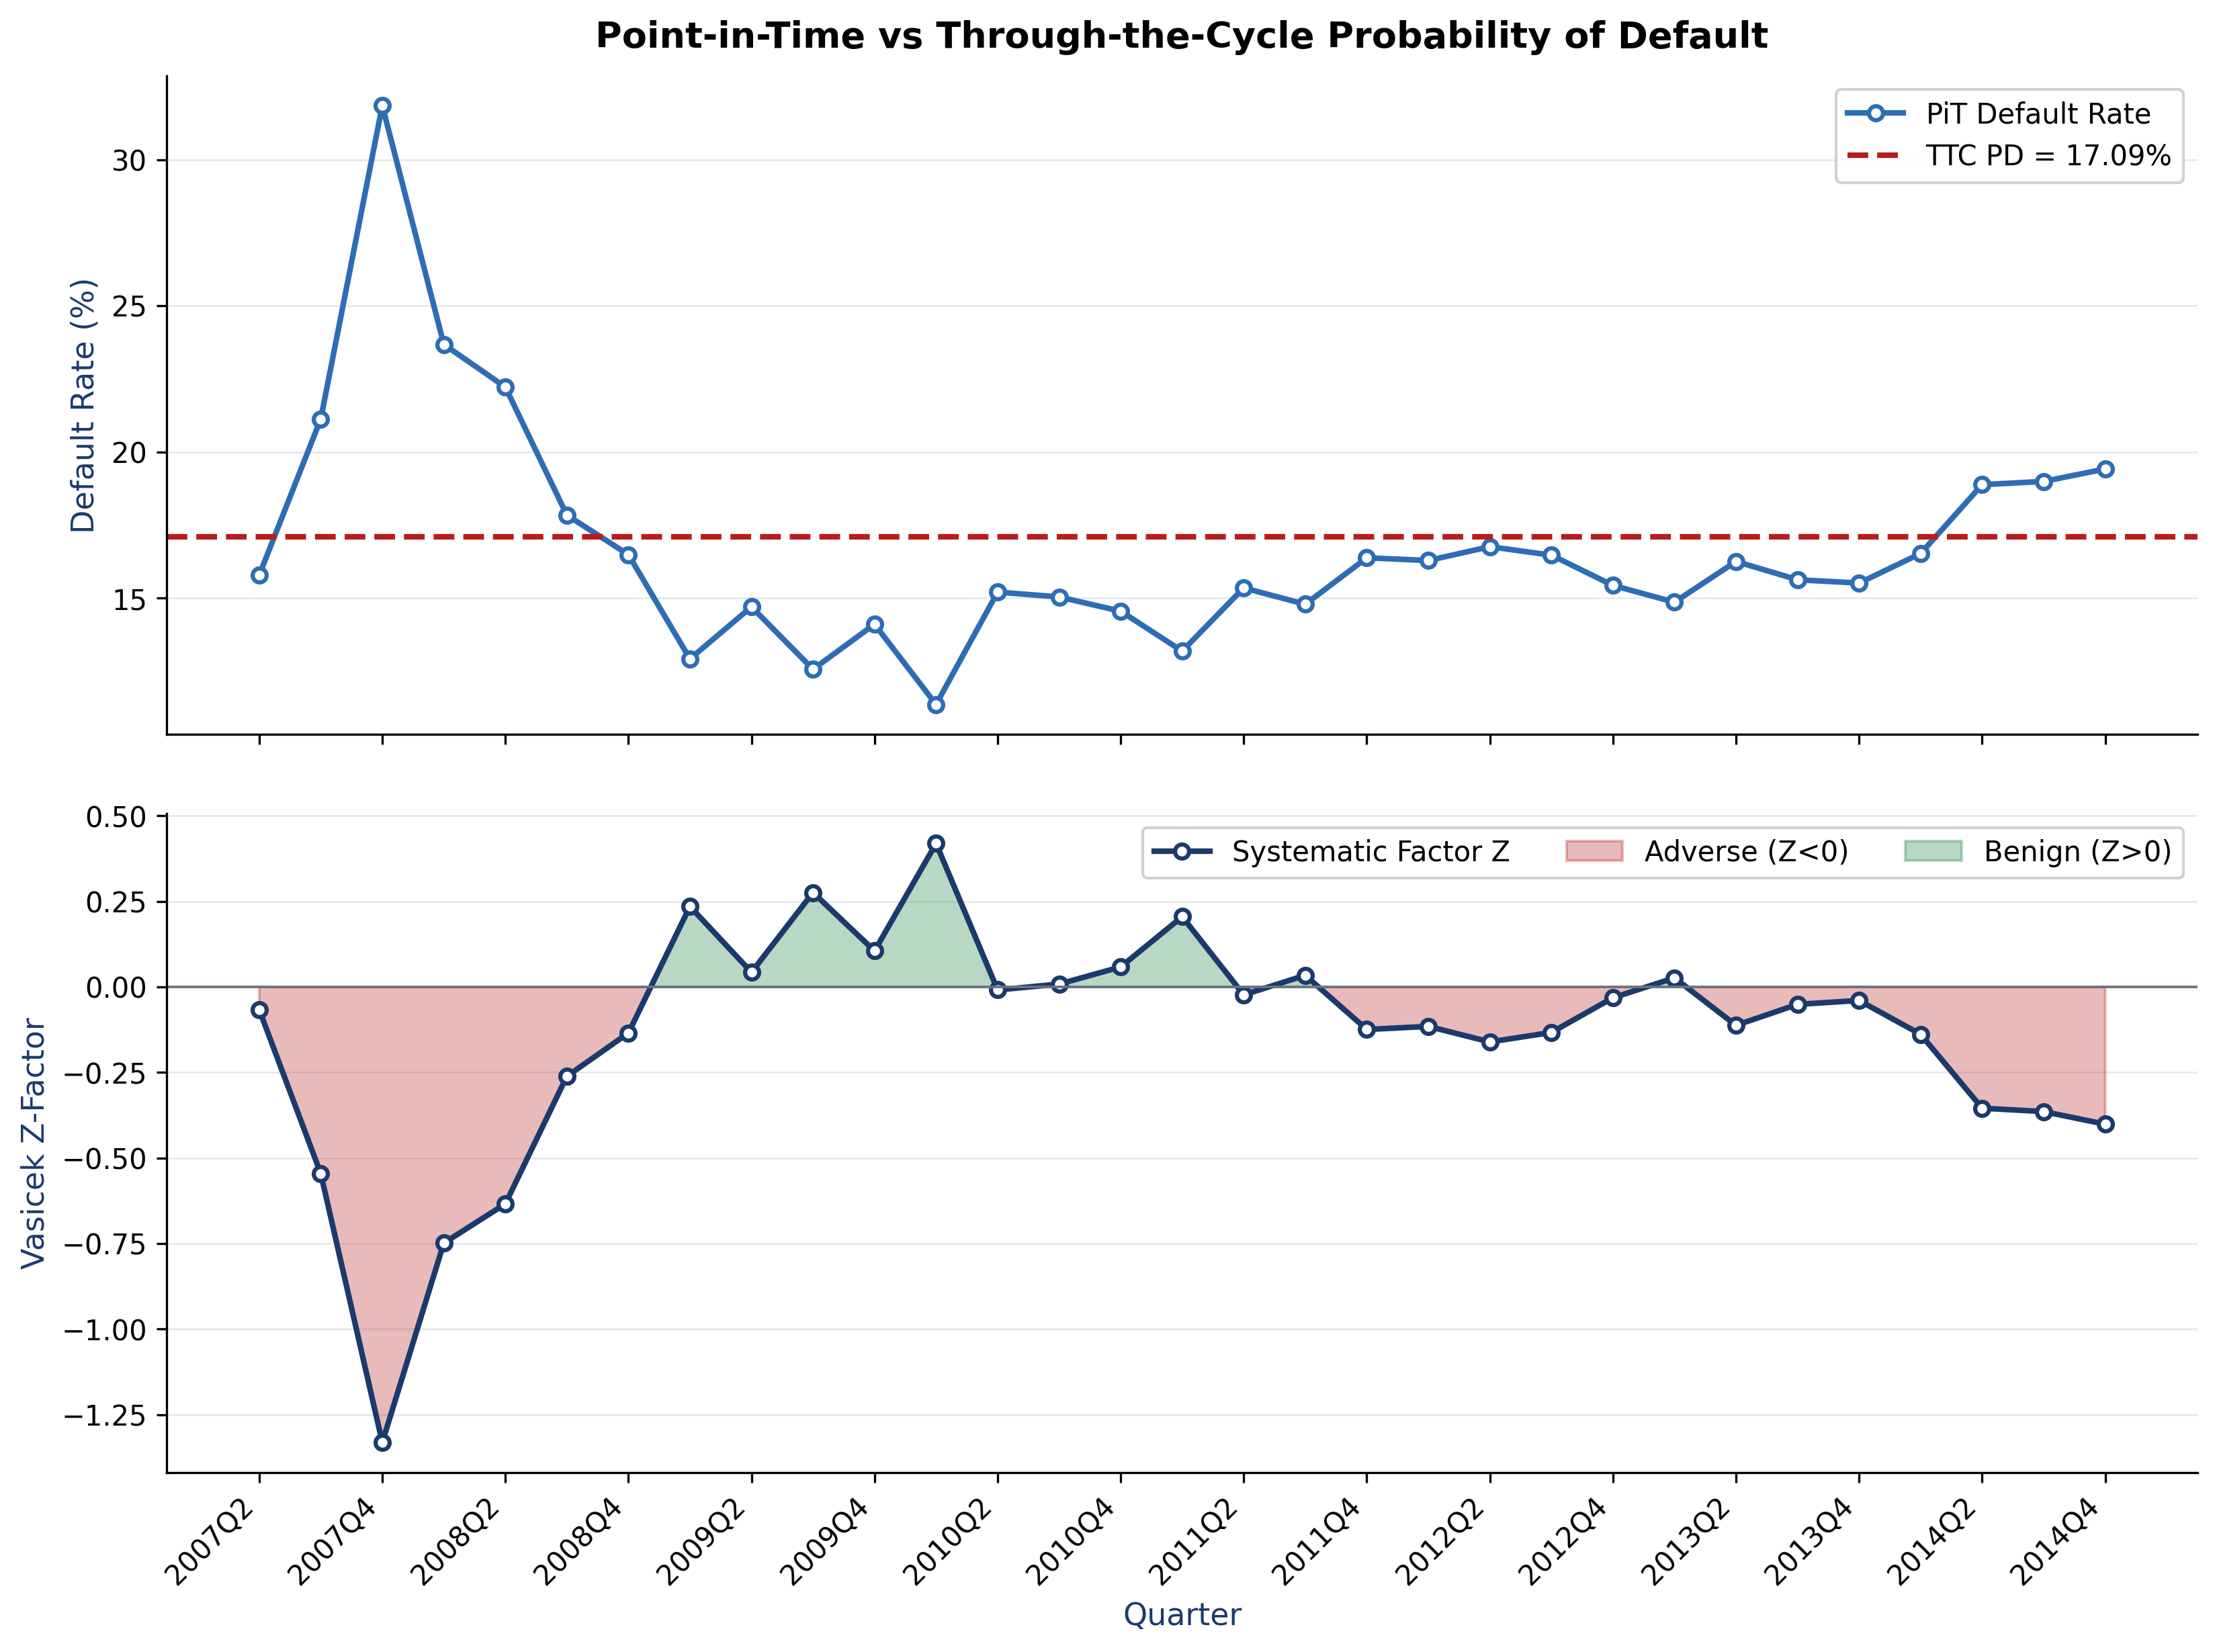
\includegraphics[width=\textwidth]{figures/pit_vs_ttc.png}
\caption{PiT vs TTC decomposition. Top: quarterly PiT default rate against the long-run TTC PD. Bottom: the implied Vasicek systematic factor $Z$, shaded by adverse/benign regime.}
\label{fig:pit_ttc}
\end{figure}

% -----------------------------------------------------------------------------
% 7. MODEL VALIDATION
% -----------------------------------------------------------------------------
\section{Model Validation}

\subsection{Discrimination Performance (OOT)}
Model validation is performed on the completely held-out Out-of-Time (OOT) dataset ($2016$--$2018$). The PD scorecard shows stable performance with an OOT AUC of \textbf{0.7003} (bootstrap 95\% CI [0.6989, 0.7017], 500 resamples) and a Kolmogorov-Smirnov (KS) statistic of \textbf{0.2894}.

\begin{figure}[H]
\centering
\begin{subfigure}[b]{0.49\textwidth}
    \centering
    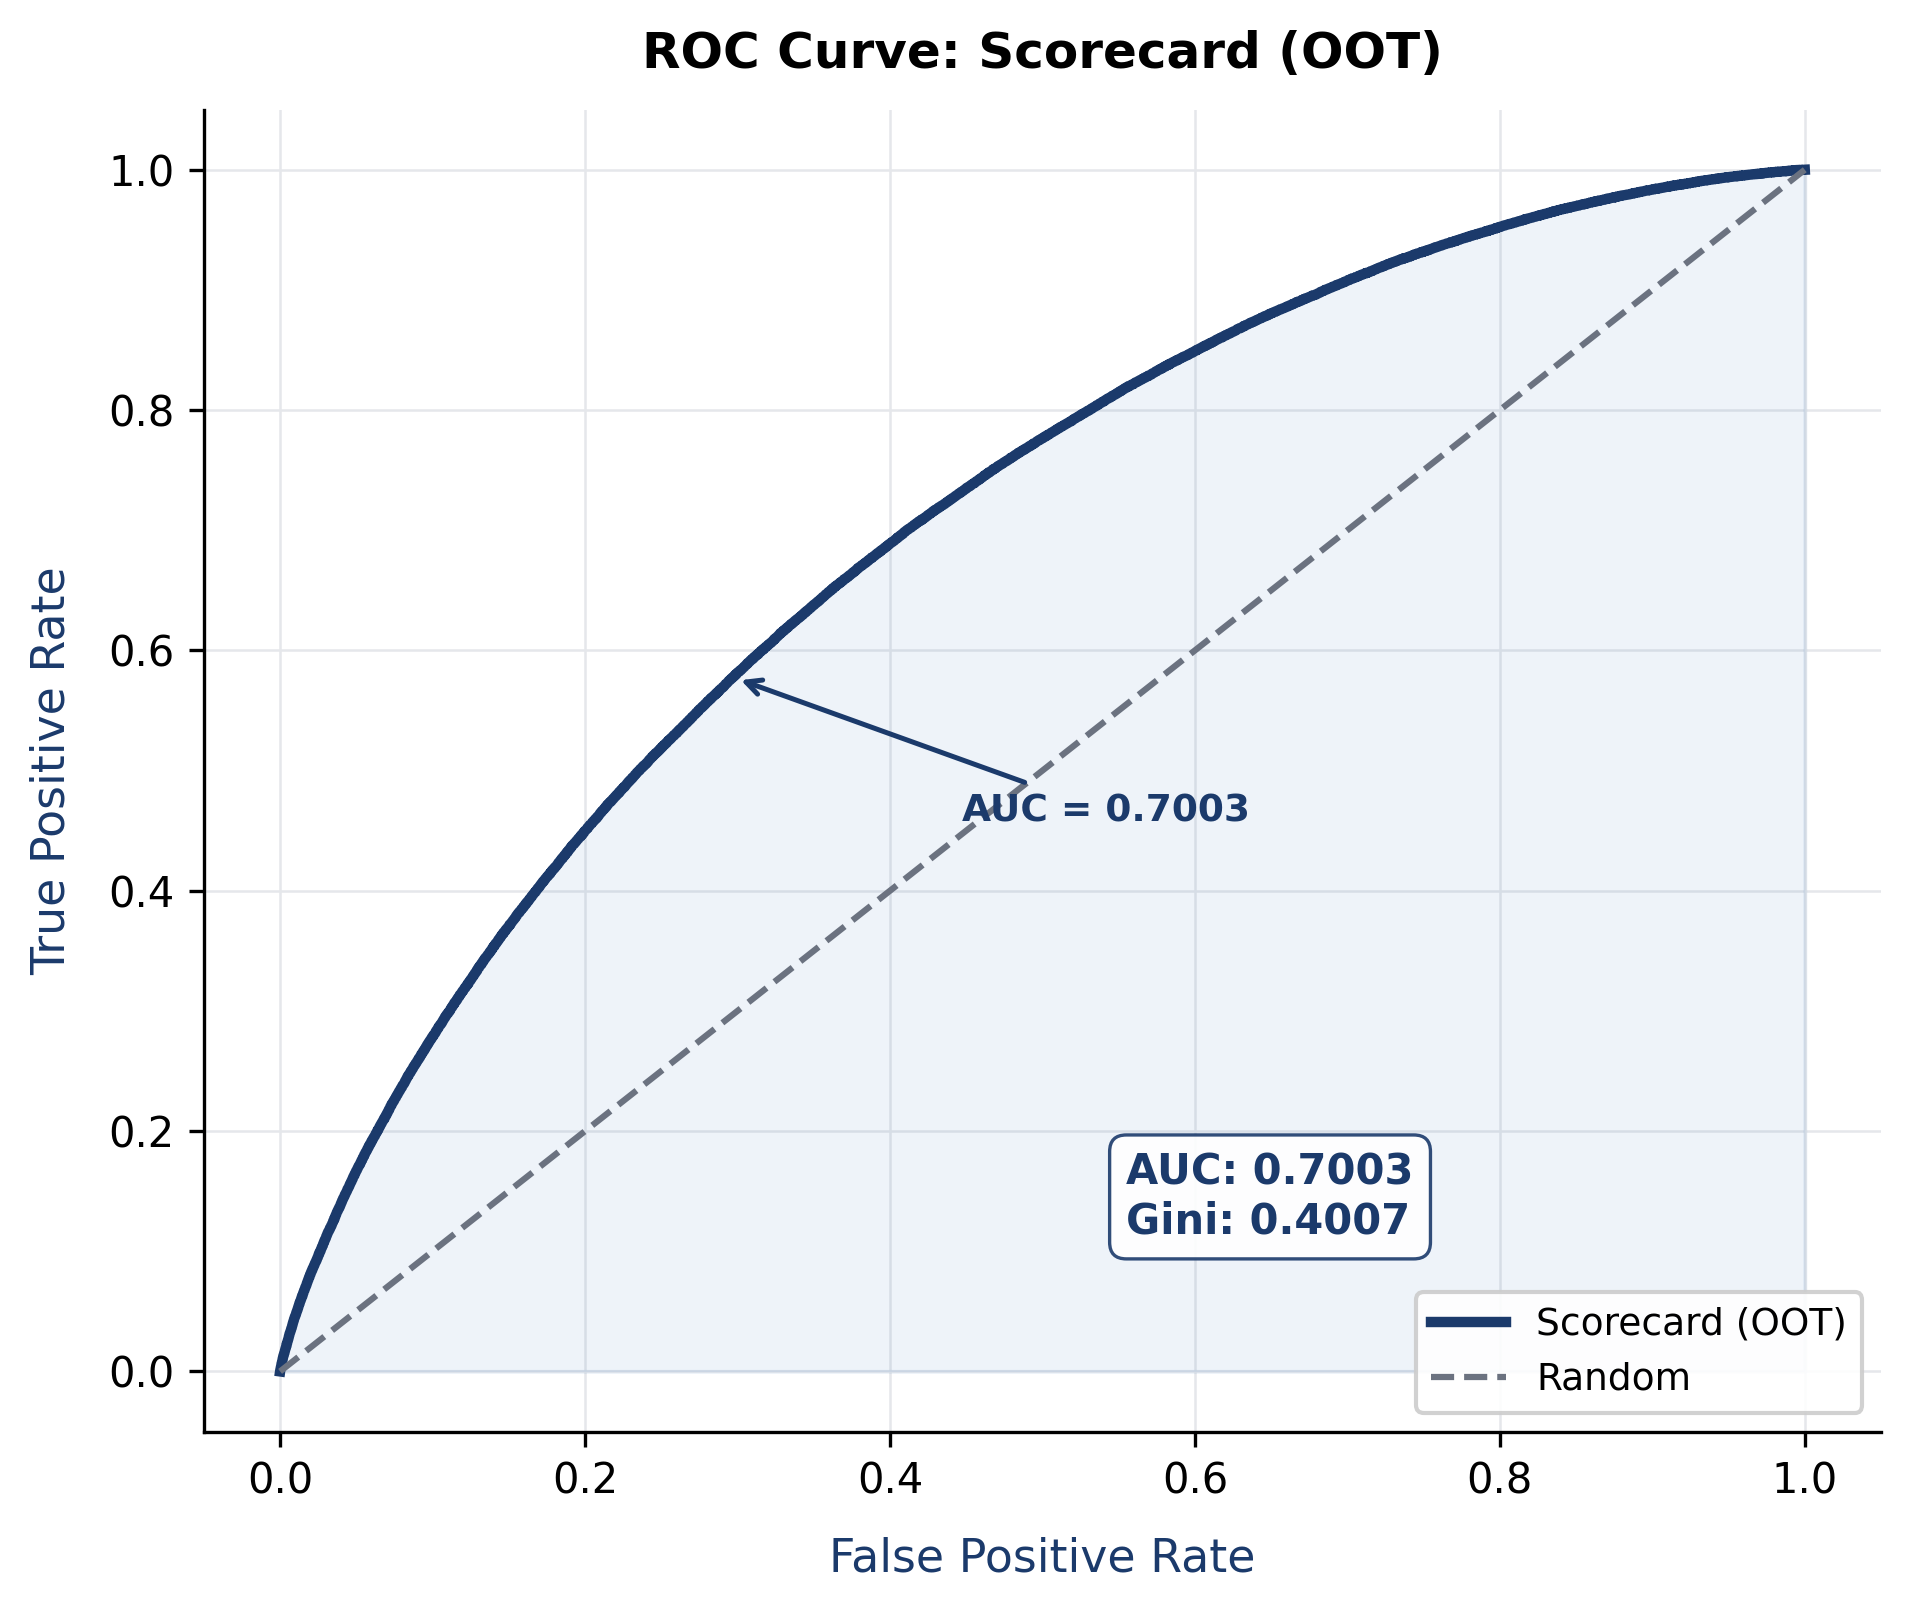
\includegraphics[width=\textwidth]{figures/validation/roc_curve_oot.png}
    \caption{OOT ROC Curve}
    \label{fig:val_roc}
\end{subfigure}
\hfill
\begin{subfigure}[b]{0.49\textwidth}
    \centering
    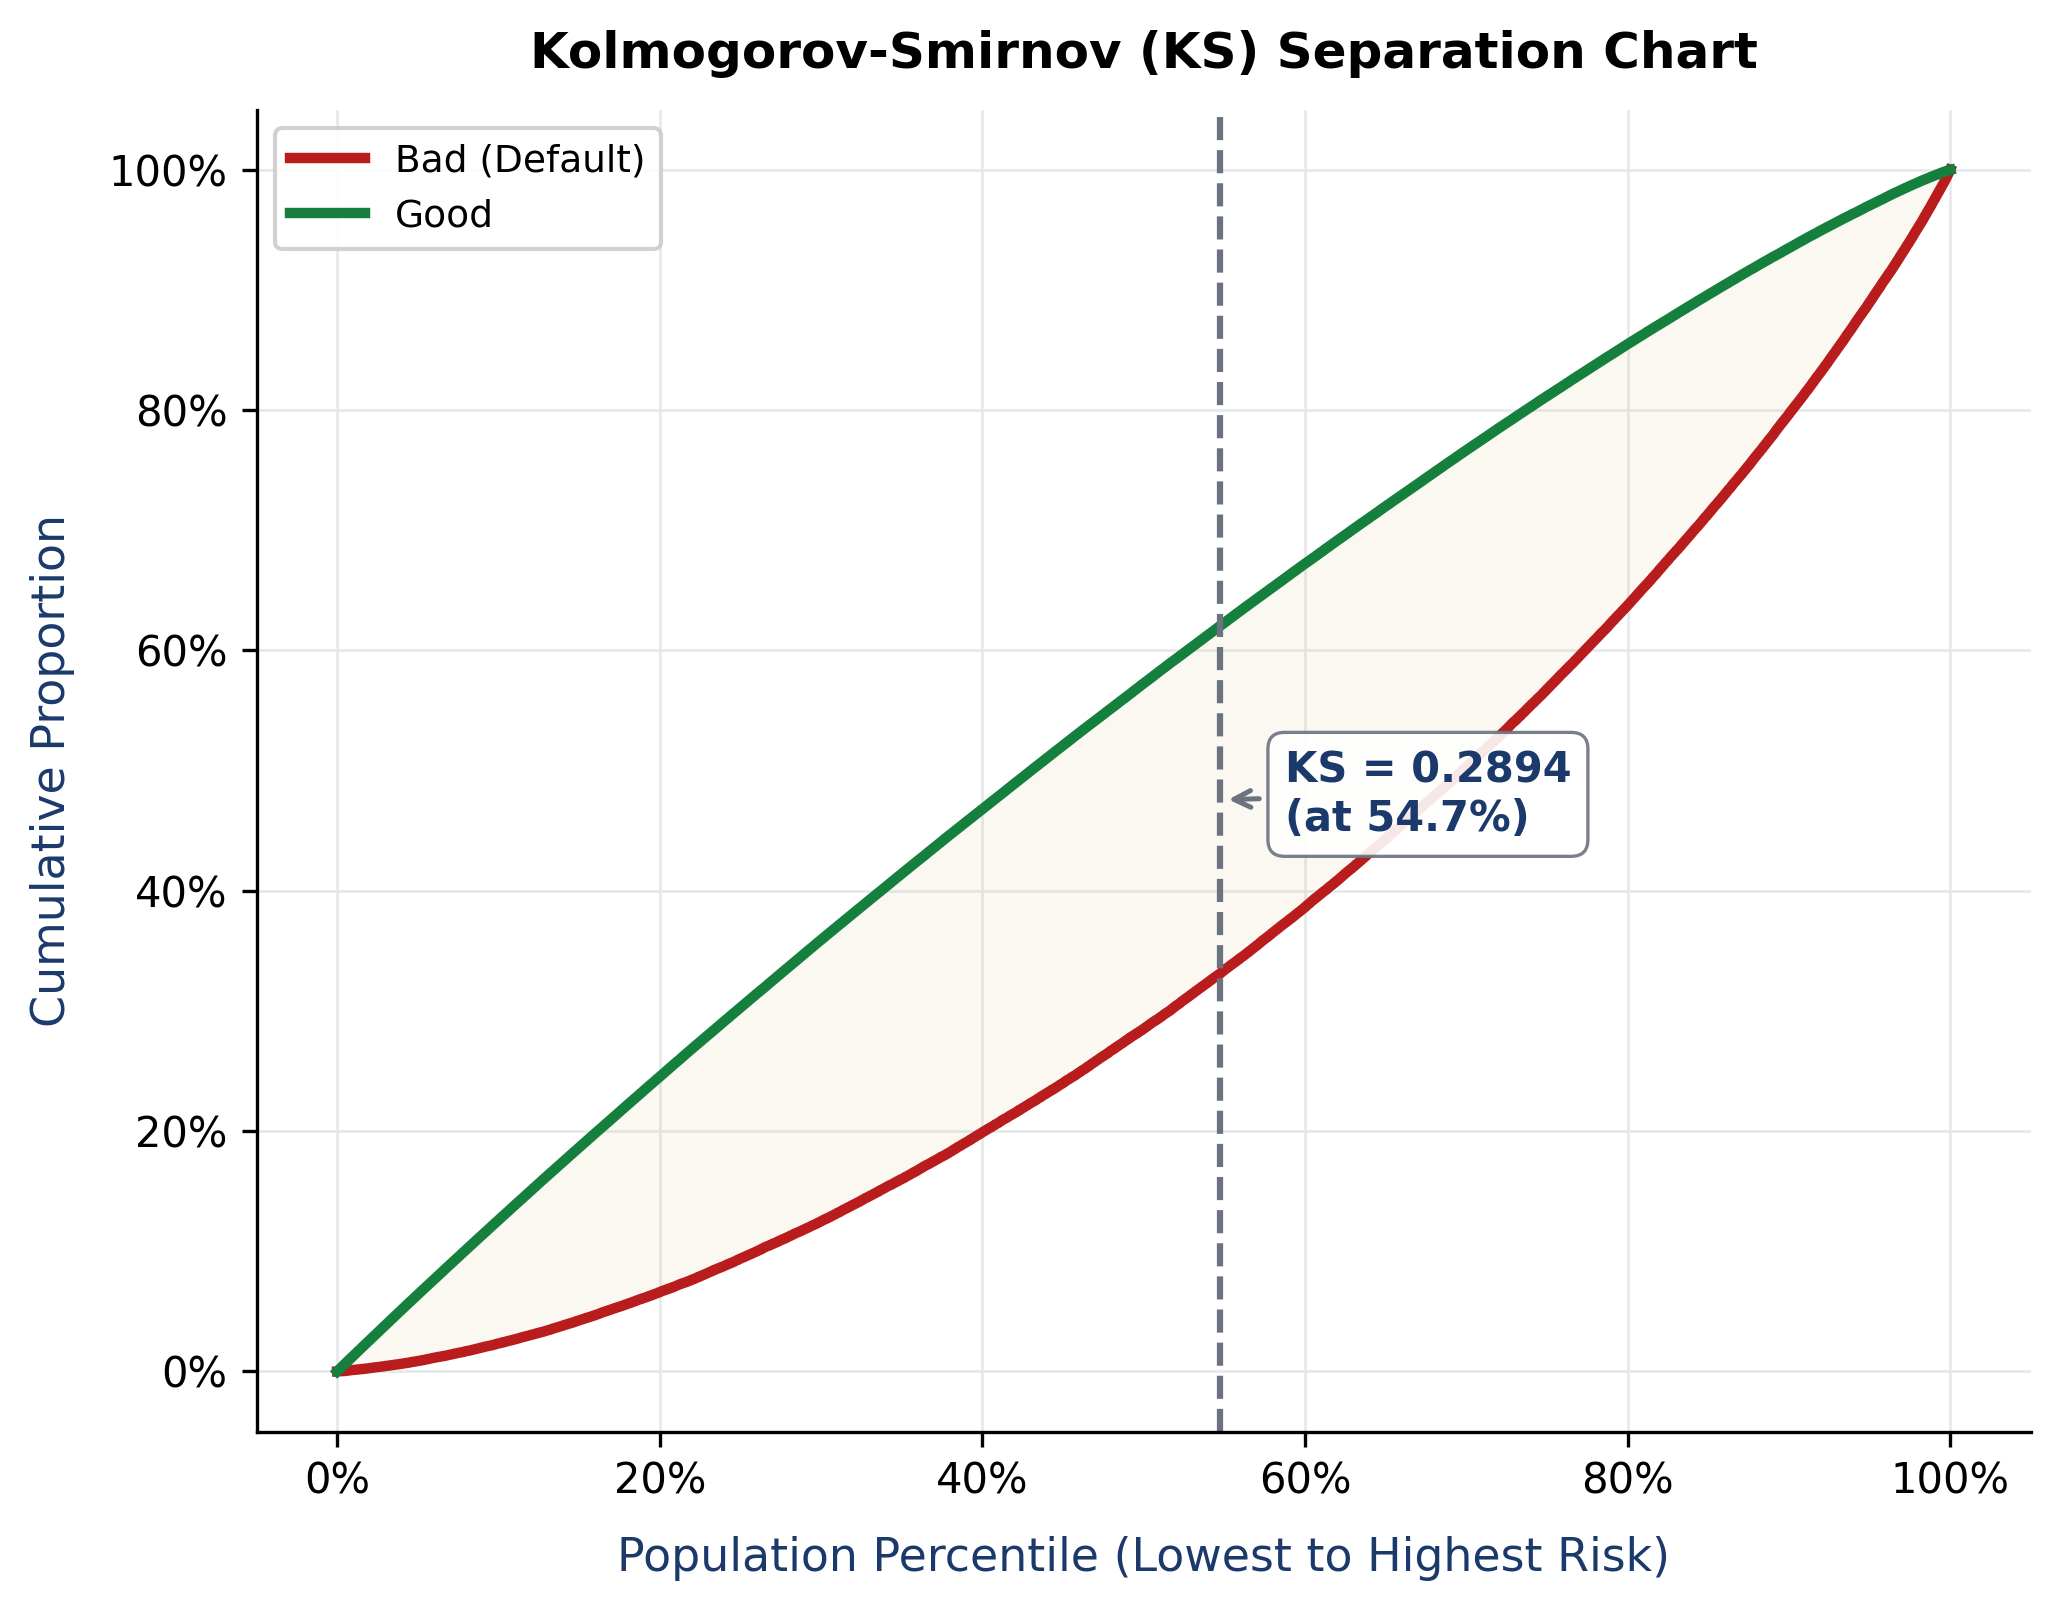
\includegraphics[width=\textwidth]{figures/validation/ks_chart_oot.png}
    \caption{OOT KS Chart}
    \label{fig:val_ks}
\end{subfigure}
\caption{Discrimination Analysis (OOT). Annotated metrics are computed on the Out-of-Time (2016--2018) population and match Table~\ref{tab:exec_summary}.}
\label{fig:val_discrimination}
\end{figure}

\subsection{Calibration Robustness}
Calibration was evaluated by comparing predicted default rates against actual observed default rates across risk deciles. The Hosmer-Lemeshow test \parencite{hosmer2013} rejects perfect calibration on the OOT dataset ($p = \text{\textbf{0.0000}} < 0.05$). Given the very large sample size ($N = \text{538,515}$), this result partly reflects the high sensitivity of the chi-squared goodness-of-fit test, but the calibration plots also indicate systematic underprediction at higher risk deciles. The statistic itself is computed on subsamples of 5,000 rows rather than the full slice --- at this $N$ it rejects on any trivial departure --- and is reported as the median over 9 independent draws, and across those replicates the $p$-value ranges from 0.0000 to 0.0000. The recalibration gate below keys off that median, so the decision does not rest on a single draw. The Spiegelhalter $Z$-test, which unlike Hosmer-Lemeshow requires no binning, returns $Z=171.71$ ($p<0.0001$) and therefore agrees with Hosmer-Lemeshow. Recalibration is governed by an out-of-time gate. The OOT window is split chronologically: the earlier 277,705 loans form the fitting slice and the later 260,810 the evaluation slice (fitting slice 2016-01-01 to 2016-11-01; evaluation slice 2016-12-01 to 2018-12-01, split on origination date). The gate \emph{triggers} on evidence of miscalibration in the fitting slice, \emph{fits} the candidate transform on that slice only, and \emph{accepts} it solely if it demonstrably improves calibration on the evaluation slice, which is never used for fitting. Gating on the in-time partition instead would be blind to the very era drift documented in Section~7.3 --- that test passes comfortably --- while fitting on the evaluation slice would trivially pass Hosmer-Lemeshow as an in-sample artefact. This design avoids both failure modes. On this run the gate \emph{triggered} (Hosmer-Lemeshow rejects on the fitting slice (p=0.0000); aggregate predicted/actual ratio 0.688 outside +/-10\%), selected an \emph{isotonic} transform by out-of-fold Brier score computed within the fitting slice, and \emph{accepted} it. On the held-out later slice the predicted-to-actual ratio moves from 0.631 to 0.918, the calibration intercept from 0.5430 to 0.0054, and the Brier score from 0.1878 to 0.1778. The transform \emph{is} attached to the production scorecard, so the PDs feeding Expected Loss, Basel RWA and IFRS~9 staging are recalibrated, but only for vintages originated in \textbf{2016} or later, which is the era the gate learned from. Earlier vintages --- \textbf{45.8\%} of loans, though only \textbf{4.35\%} of exposure by EAD, since EAD amortises to the reporting date and these are the oldest vintages --- keep their raw model PD, so the deployed PD level steps at the 2016 boundary. Because every one of those improvements is measured on vintages excluded from the fit, this is an out-of-sample result rather than an in-sample artefact. Note that the IFRS 9 lifetime PD is produced by the separate hazard model and is not passed through this transform (Section~6.2), so the ECL provisions do not inherit the correction; the known limitations in Section~10 still apply.

\begin{table}[H]
\centering
\small
\caption{Deployed Recalibration, Measured on the Held-Out Later OOT Slice}
\label{tab:calibration_comparison}
\vspace{0.5em}
\begin{tabular}{lcccc}
\toprule
\textbf{Metric} & \textbf{Target} & \textbf{Before Recalib.} & \textbf{After Recalib.} & \textbf{$\Delta$ Change} \\
\midrule
OOT AUC & --- & 0.6912 & 0.6911 & -0.0001 \\
Brier Score & $<0.25$ & 0.1878 & 0.1778 & -0.0100 \checkmark \\
Calibration Slope & $\approx 1.00$ & 0.9371 & 0.8819 & -0.0552 $\times$ \\
Calibration Intercept & $\approx 0.00$ & 0.5430 & 0.0054 & -0.5376 \checkmark \\
Expected Default Rate & = Actual & 16.61\% & 24.18\% & +7.57\% \checkmark \\
Actual Default Rate & 26.33\% & 26.33\% & 26.33\% & +0.00\% \\
Hosmer-Lemeshow $p$ & $>0.05$ & 0.0000 & 0.0006 & $\ast$ below 0.05 \\
\bottomrule
\multicolumn{5}{p{\linewidth}}{\footnotesize \checkmark\ marks a metric that moved \emph{toward} its target and $\times$ one that moved away. This table measures the \emph{deployed} transform (isotonic), fitted on the earlier oot slice and evaluated on the disjoint later slice of 260,810 loans spanning 2016-12-01 to 2018-12-01 --- the same evidence the acceptance decision was made on, so the table and the narrative above cannot disagree. Note the trade-off: the calibration slope moved away from target while the level measures improved sharply. This is characteristic of isotonic recalibration, which is a monotone step function fitted to the aggregate level and is not constrained to preserve the logit-scale slope. The gate accepts on the aggregate ratio and the Brier score, both of which improved.} \\
\end{tabular}
\end{table}

\begin{figure}[H]
\centering
\begin{subfigure}[b]{0.49\textwidth}
    \centering
    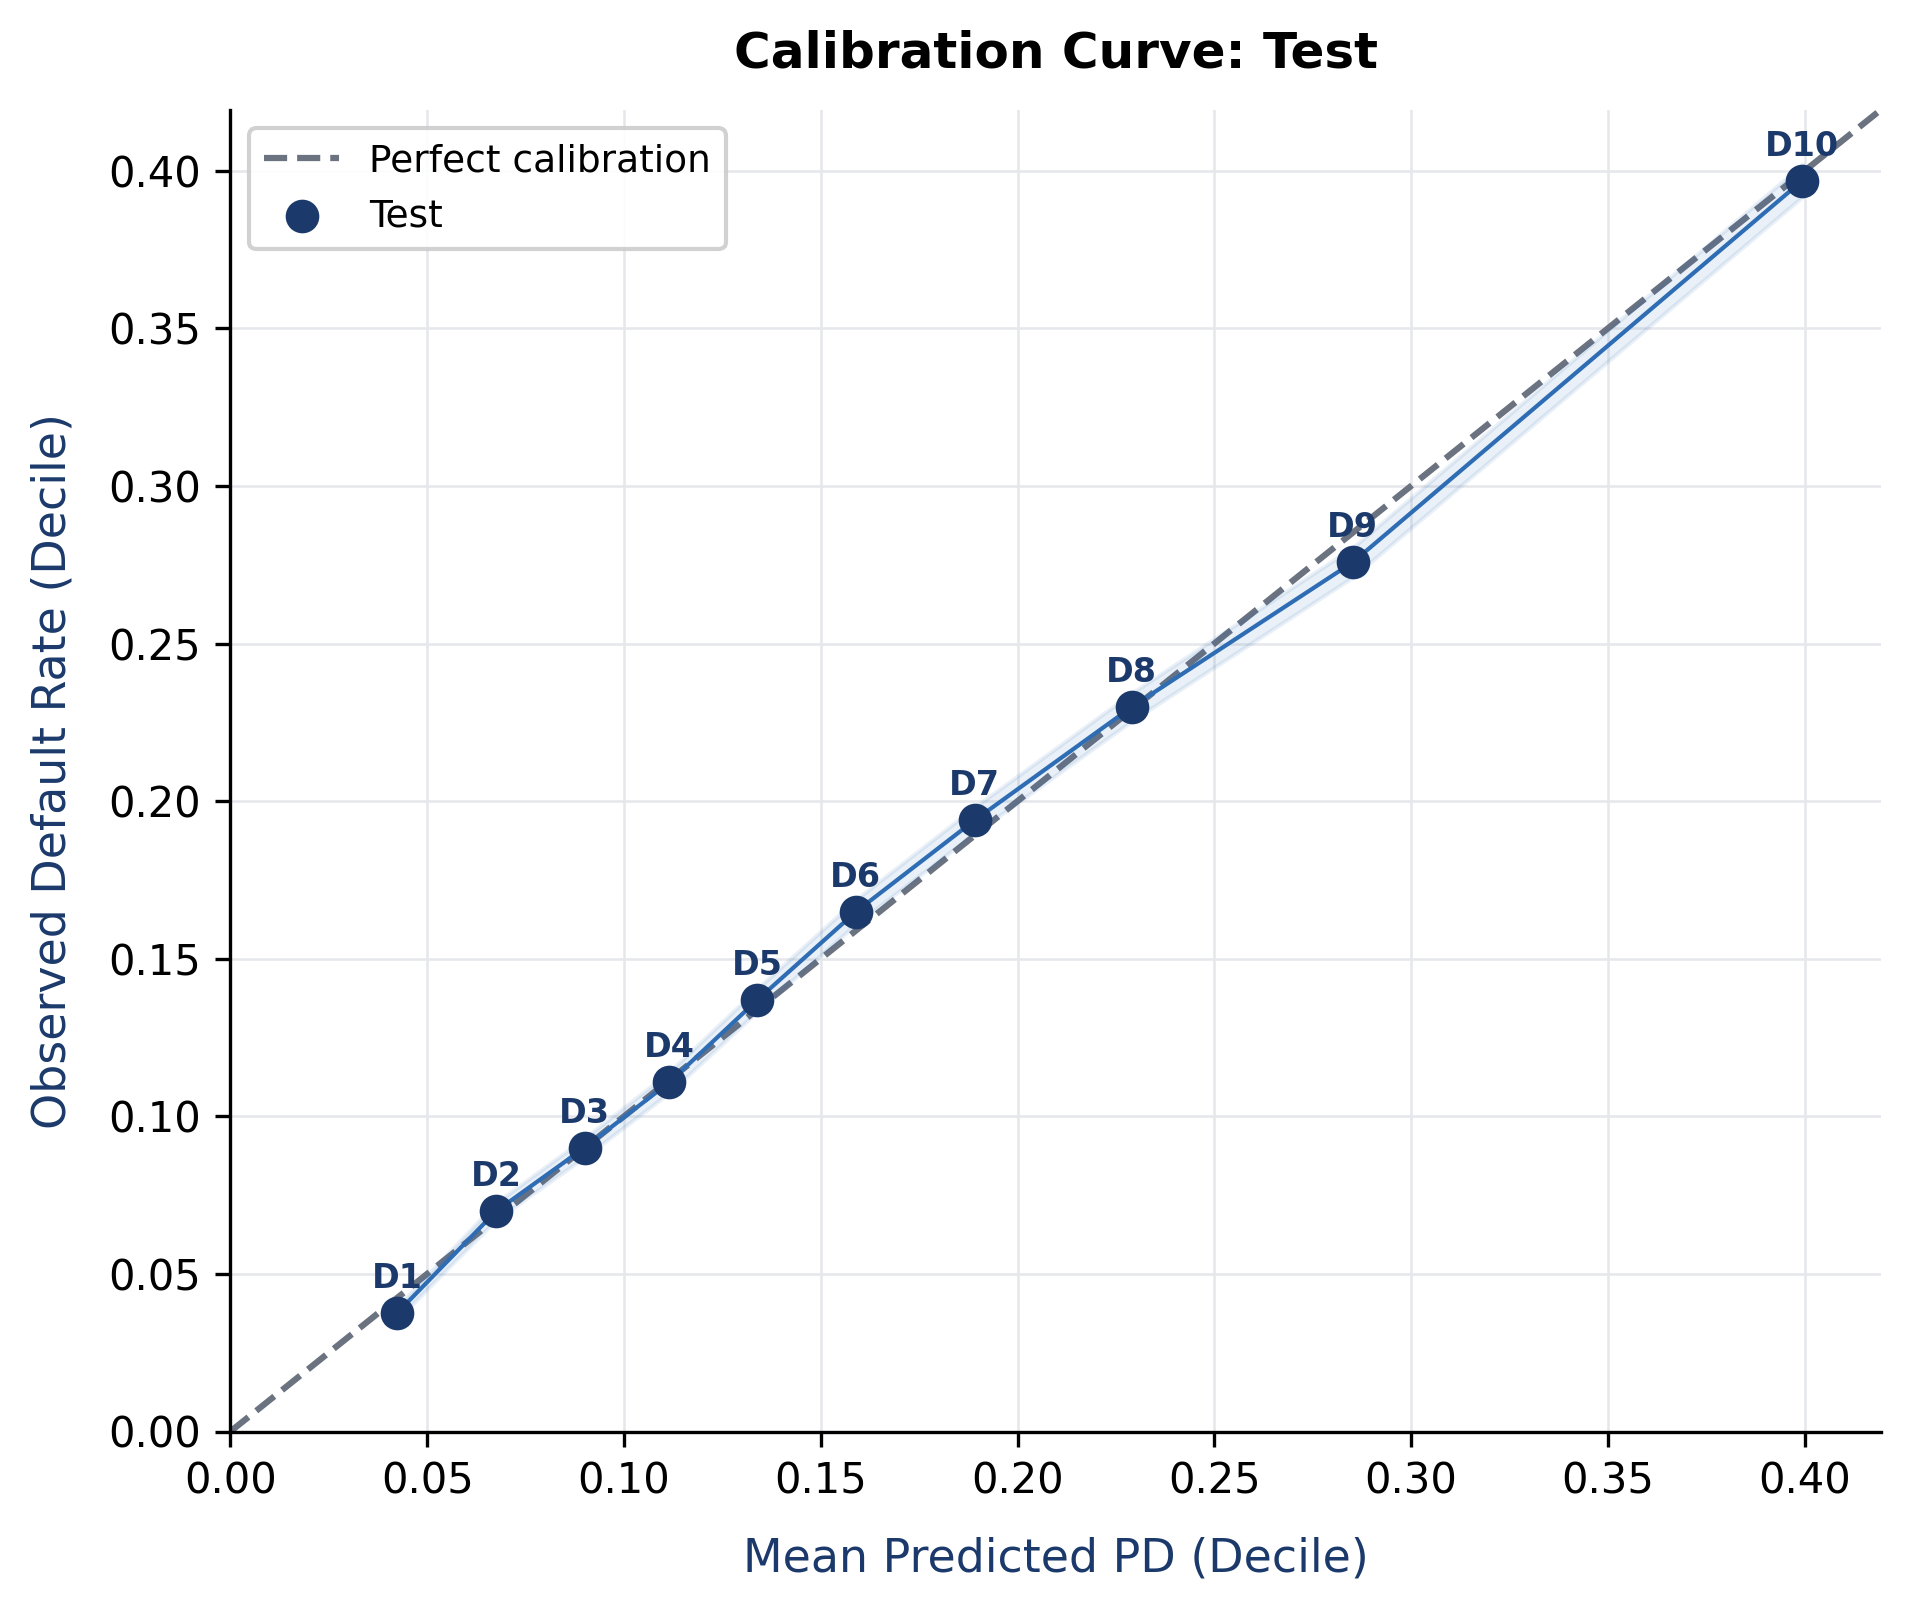
\includegraphics[width=\textwidth]{figures/validation/calibration_test.png}
    \caption{Calibration (In-Time Test Set)}
    \label{fig:cal_test}
\end{subfigure}
\hfill
\begin{subfigure}[b]{0.49\textwidth}
    \centering
    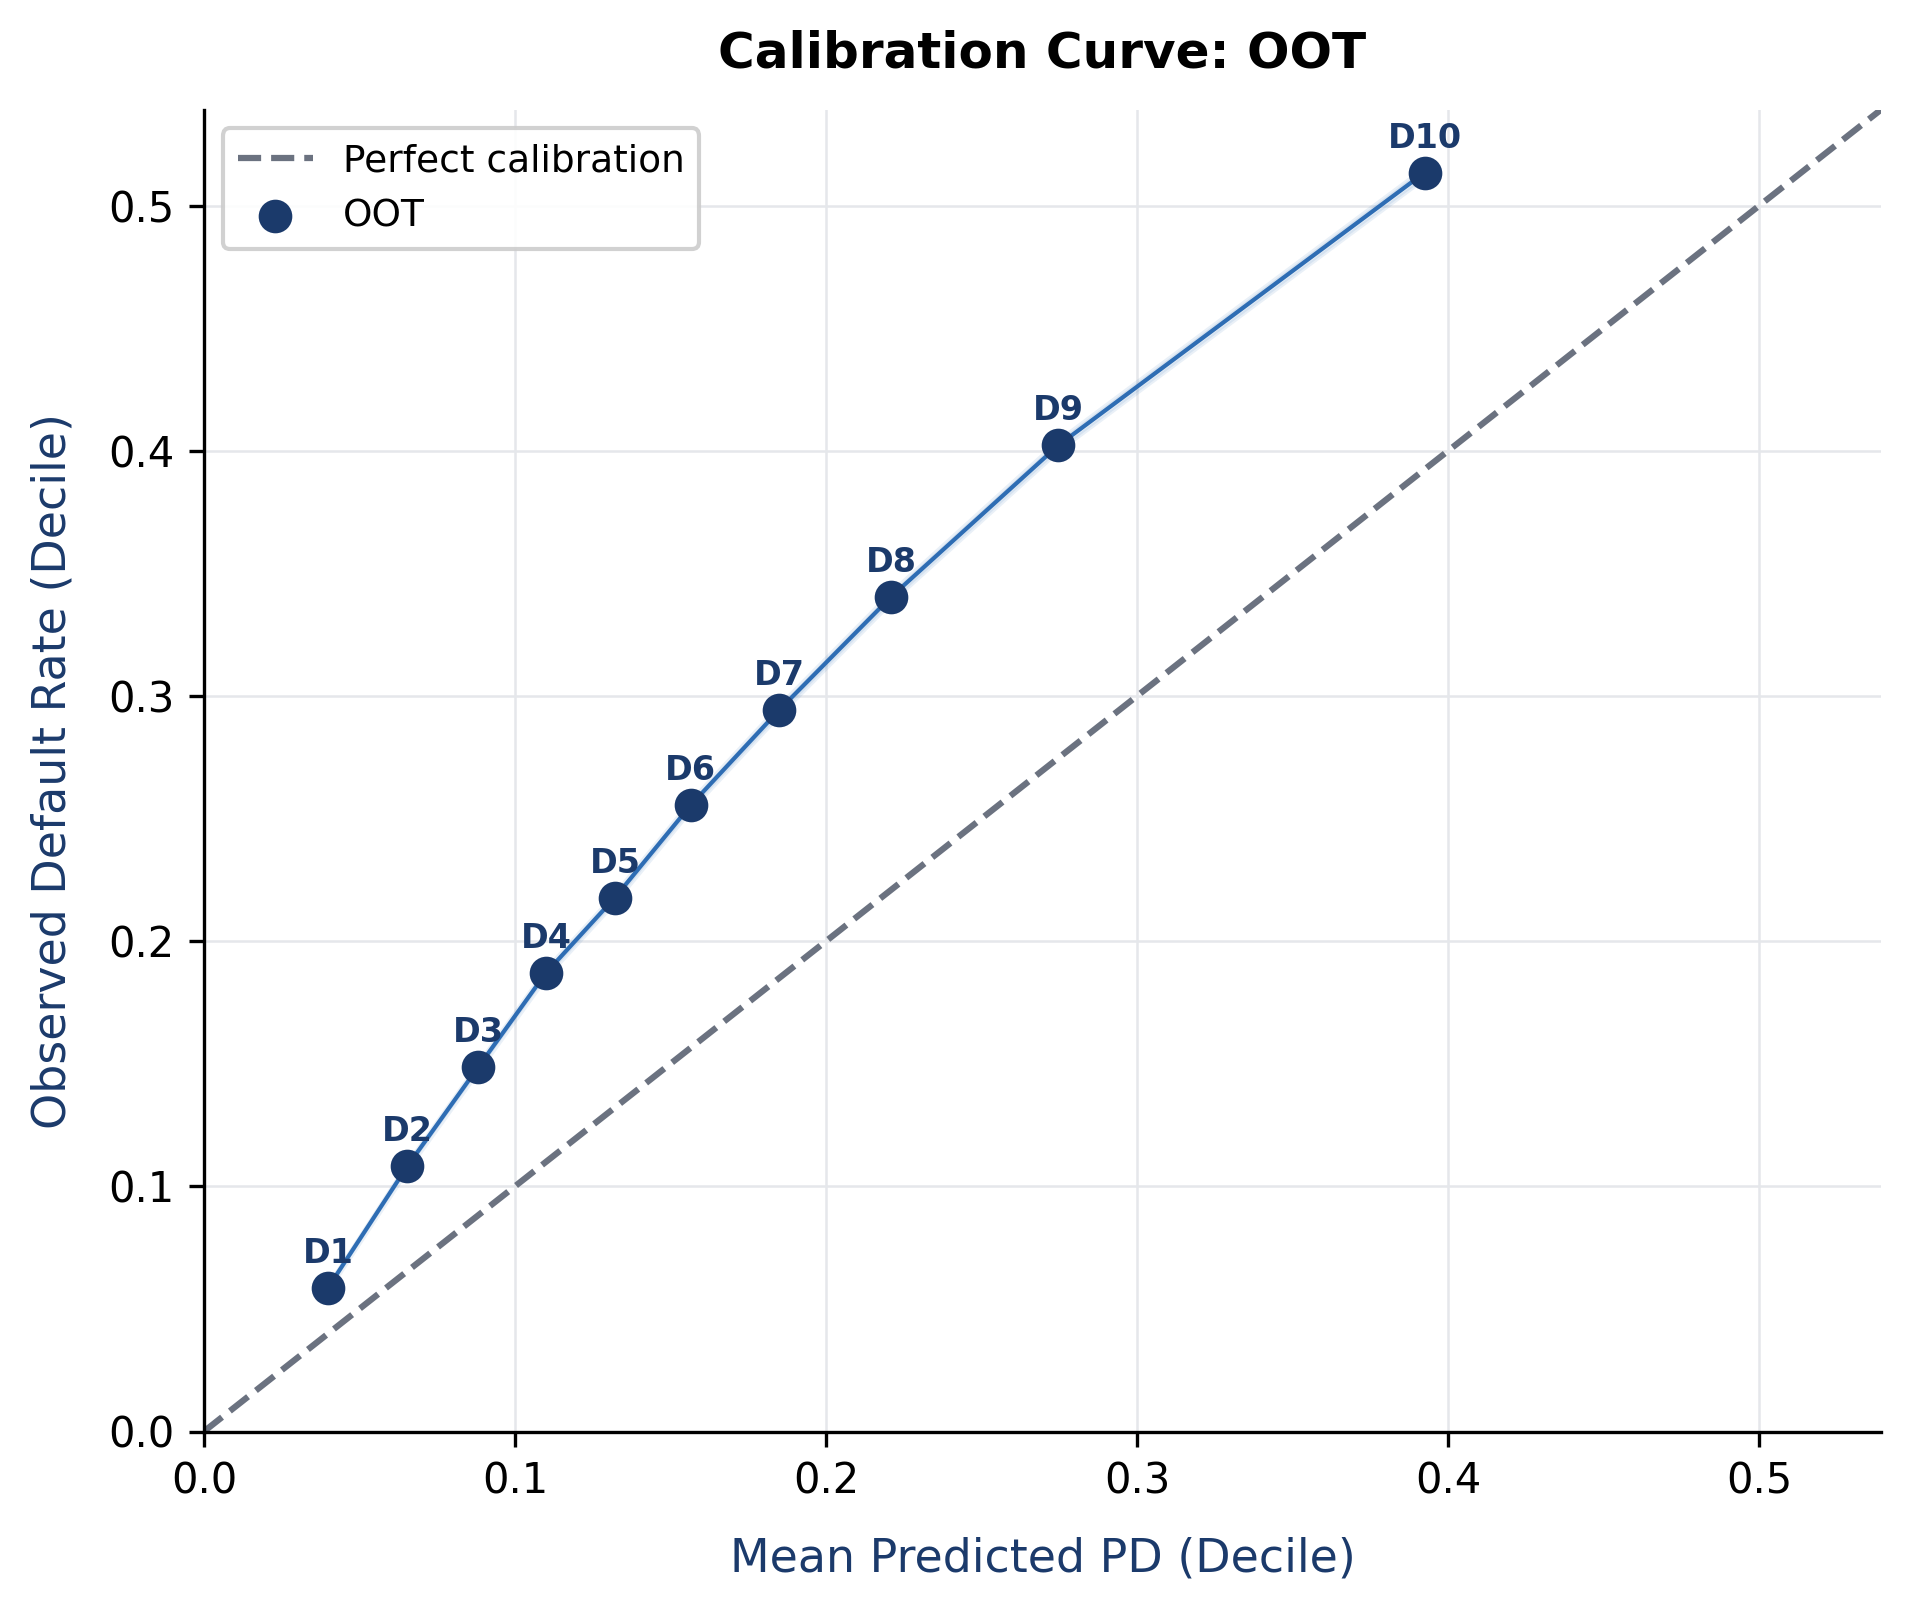
\includegraphics[width=\textwidth]{figures/validation/calibration_oot.png}
    \caption{Calibration (Out-of-Time Validation)}
    \label{fig:cal_oot}
\end{subfigure}
\caption{Calibration Curves}
\label{fig:val_calibration}
\end{figure}

\subsection{Backtesting and Vintage Calibration}

Model backtesting compares the scorecard's predicted average PD against observed default rates segmented by quarterly origination vintage, following the methodology of \parencite{eba2017} and \parencite{bcbs2005}. For each vintage cohort, we assess whether the predicted mean PD lies within the tolerance band $[0.80, 1.25]$ of the realised default frequency:
\begin{equation}
\text{PD Ratio}_{v} = \frac{\bar{p}_v}{\bar{d}_v}
\end{equation}
where $\bar{p}_v$ is the cohort-average predicted PD and $\bar{d}_v$ is the realised default rate. A ratio inside $[0.80, 1.25]$ indicates acceptable calibration; cohorts outside it are flagged for recalibration ($\dagger$). That band, the flag in the table below and the count in the next paragraph all come from one constant in \texttt{validation/backtest.py} --- this passage previously described a 50\% band, counted vintages against $[0.80, 1.25]$, and was implemented twice with a third pair of thresholds. Table~\ref{tab:pd_backtest} reports the backtesting results by origination year, exposure-weighted across that year's quarters. The ratios below describe the PDs the pipeline actually deploys rather than raw model output --- which for in-scope vintages means \textbf{post-recalibration}. Rows before 2016 are outside the recalibrator's vintage scope (Section~7.2) and are therefore raw model output; the two halves of the table are not the same estimator.

Of the 11 origination years backtested, 9 sit inside the $[0.80, 1.25]$ predicted-to-actual band, 2 under-predict (2007, 2008, lowest 0.61). This pattern is the calibration drift identified in Section~7.2, and corrected in production by the isotonic transform that the out-of-time gate accepted (Section~7.2), applied to the scorecard's 12-month PD feeding Expected Loss, Basel RWA and SICR staging for 2016+ vintages only. The hazard model's \textbf{lifetime} PD that drives IFRS~9 ECL directly ($\text{ECL} = \sum_t m(t)\times\text{LGD}(t)\times\text{EAD}(t)/(1+\text{EIR})^t$) is a separate estimator and is \emph{not} passed through this scorecard recalibration; it is instead independently validated against realised lifetime default rates by vintage in Table~\ref{tab:lifetime_pd_calibration} (Section~6.2).

\begin{table}[H]
\centering
\footnotesize
\setlength{\tabcolsep}{4pt}
\caption{Vintage PD Backtesting: Predicted vs Realised Default Rate}
\label{tab:pd_backtest}
\vspace{0.5em}
\begin{tabular}{lcccc}
\toprule
\textbf{Vintage (Q)} & \textbf{N Loans} & \textbf{Predicted PD} & \textbf{Actual DR [95\% CI]} & \textbf{PD Ratio} \\
\midrule
2007 & 603 & 15.86\% & 26.20\% [22.9\%, 29.9\%] & 0.61 {\checkmark} \\
2008 & 2,393 & 13.57\% & 20.73\% [19.2\%, 22.4\%] & 0.65 {\checkmark} \\
2009 & 5,281 & 11.45\% & 13.69\% [12.8\%, 14.6\%] & 0.84 {\checkmark} \\
2010 & 12,537 & 13.99\% & 14.01\% [13.4\%, 14.6\%] & 1.00 {\checkmark} \\
2011 & 21,721 & 14.55\% & 15.18\% [14.7\%, 15.7\%] & 0.96 {\checkmark} \\
2012 & 53,367 & 15.51\% & 16.20\% [15.9\%, 16.5\%] & 0.96 {\checkmark} \\
2013 & 134,807 & 17.17\% & 15.60\% [15.4\%, 15.8\%] & 1.10 {\checkmark} \\
2014 & 223,437 & 18.01\% & 18.57\% [18.4\%, 18.7\%] & 0.97 {\checkmark} \\
2016 & 297,651 & 24.32\% & 24.46\% [24.3\%, 24.6\%] & 0.99 {\checkmark} \\
2017 & 177,325 & 24.34\% & 26.60\% [26.4\%, 26.8\%] & 0.91 {\checkmark} \\
2018 & 63,539 & 23.45\% & 25.33\% [25.0\%, 25.7\%] & 0.93 {\checkmark} \\
\bottomrule
\end{tabular}
\end{table}

\subsubsection*{Era-Specific Recalibration of the Vintage Drift}
A single global recalibrator cannot correct an era-specific bias. We therefore fit separate isotonic and Platt recalibrators for the pre-2016 and 2016--2018 eras and measure, per vintage group, the raw and recalibrated PD ratio against the realised default rate (Table~\ref{tab:vintage_calib}, Figure~\ref{fig:vintage_calib}). The raw ratio is materially below $1.0$ for the newer vintages (the documented under-prediction), and the era-specific isotonic recalibration moves it back toward $1.0$. This is an in-sample diagnostic that quantifies the drift and demonstrates the correction; production PD is unchanged. Since the era-specific calibrators are fitted and evaluated on the same vintage partitions (e.g. 2016--2018), the resulting alignment (Isotonic/Platt PD equals the Actual DR exactly) is in-sample and tautological: it is a diagnostic baseline that demonstrates the extent of the raw model's drift, not a validation of the recalibrator's out-of-sample generalization.

\begin{table}[H]
\centering
\caption{Calibration by Vintage Group --- Raw vs Era-Recalibrated PD}
\label{tab:vintage_calib}
\vspace{0.5em}
\begin{tabular}{lrrrrrr}
\toprule
\textbf{Vintage} & \textbf{N} & \textbf{Raw PD} & \textbf{Isotonic PD} & \textbf{Platt PD} & \textbf{Actual DR} & \textbf{Raw Ratio} \\
\midrule
2007-2012 & 95,902 & 14.83\% & 14.84\% & 14.91\% & 15.72\% & 0.943 \\
2013-2014 & 358,244 & 17.69\% & 17.69\% & 17.67\% & 17.45\% & 1.014 \\
2016-2018 & 538,515 & 24.23\% & 25.27\% & 25.28\% & 25.27\% & 0.959 \\
\bottomrule
\end{tabular}
\end{table}

\begin{figure}[H]
\centering
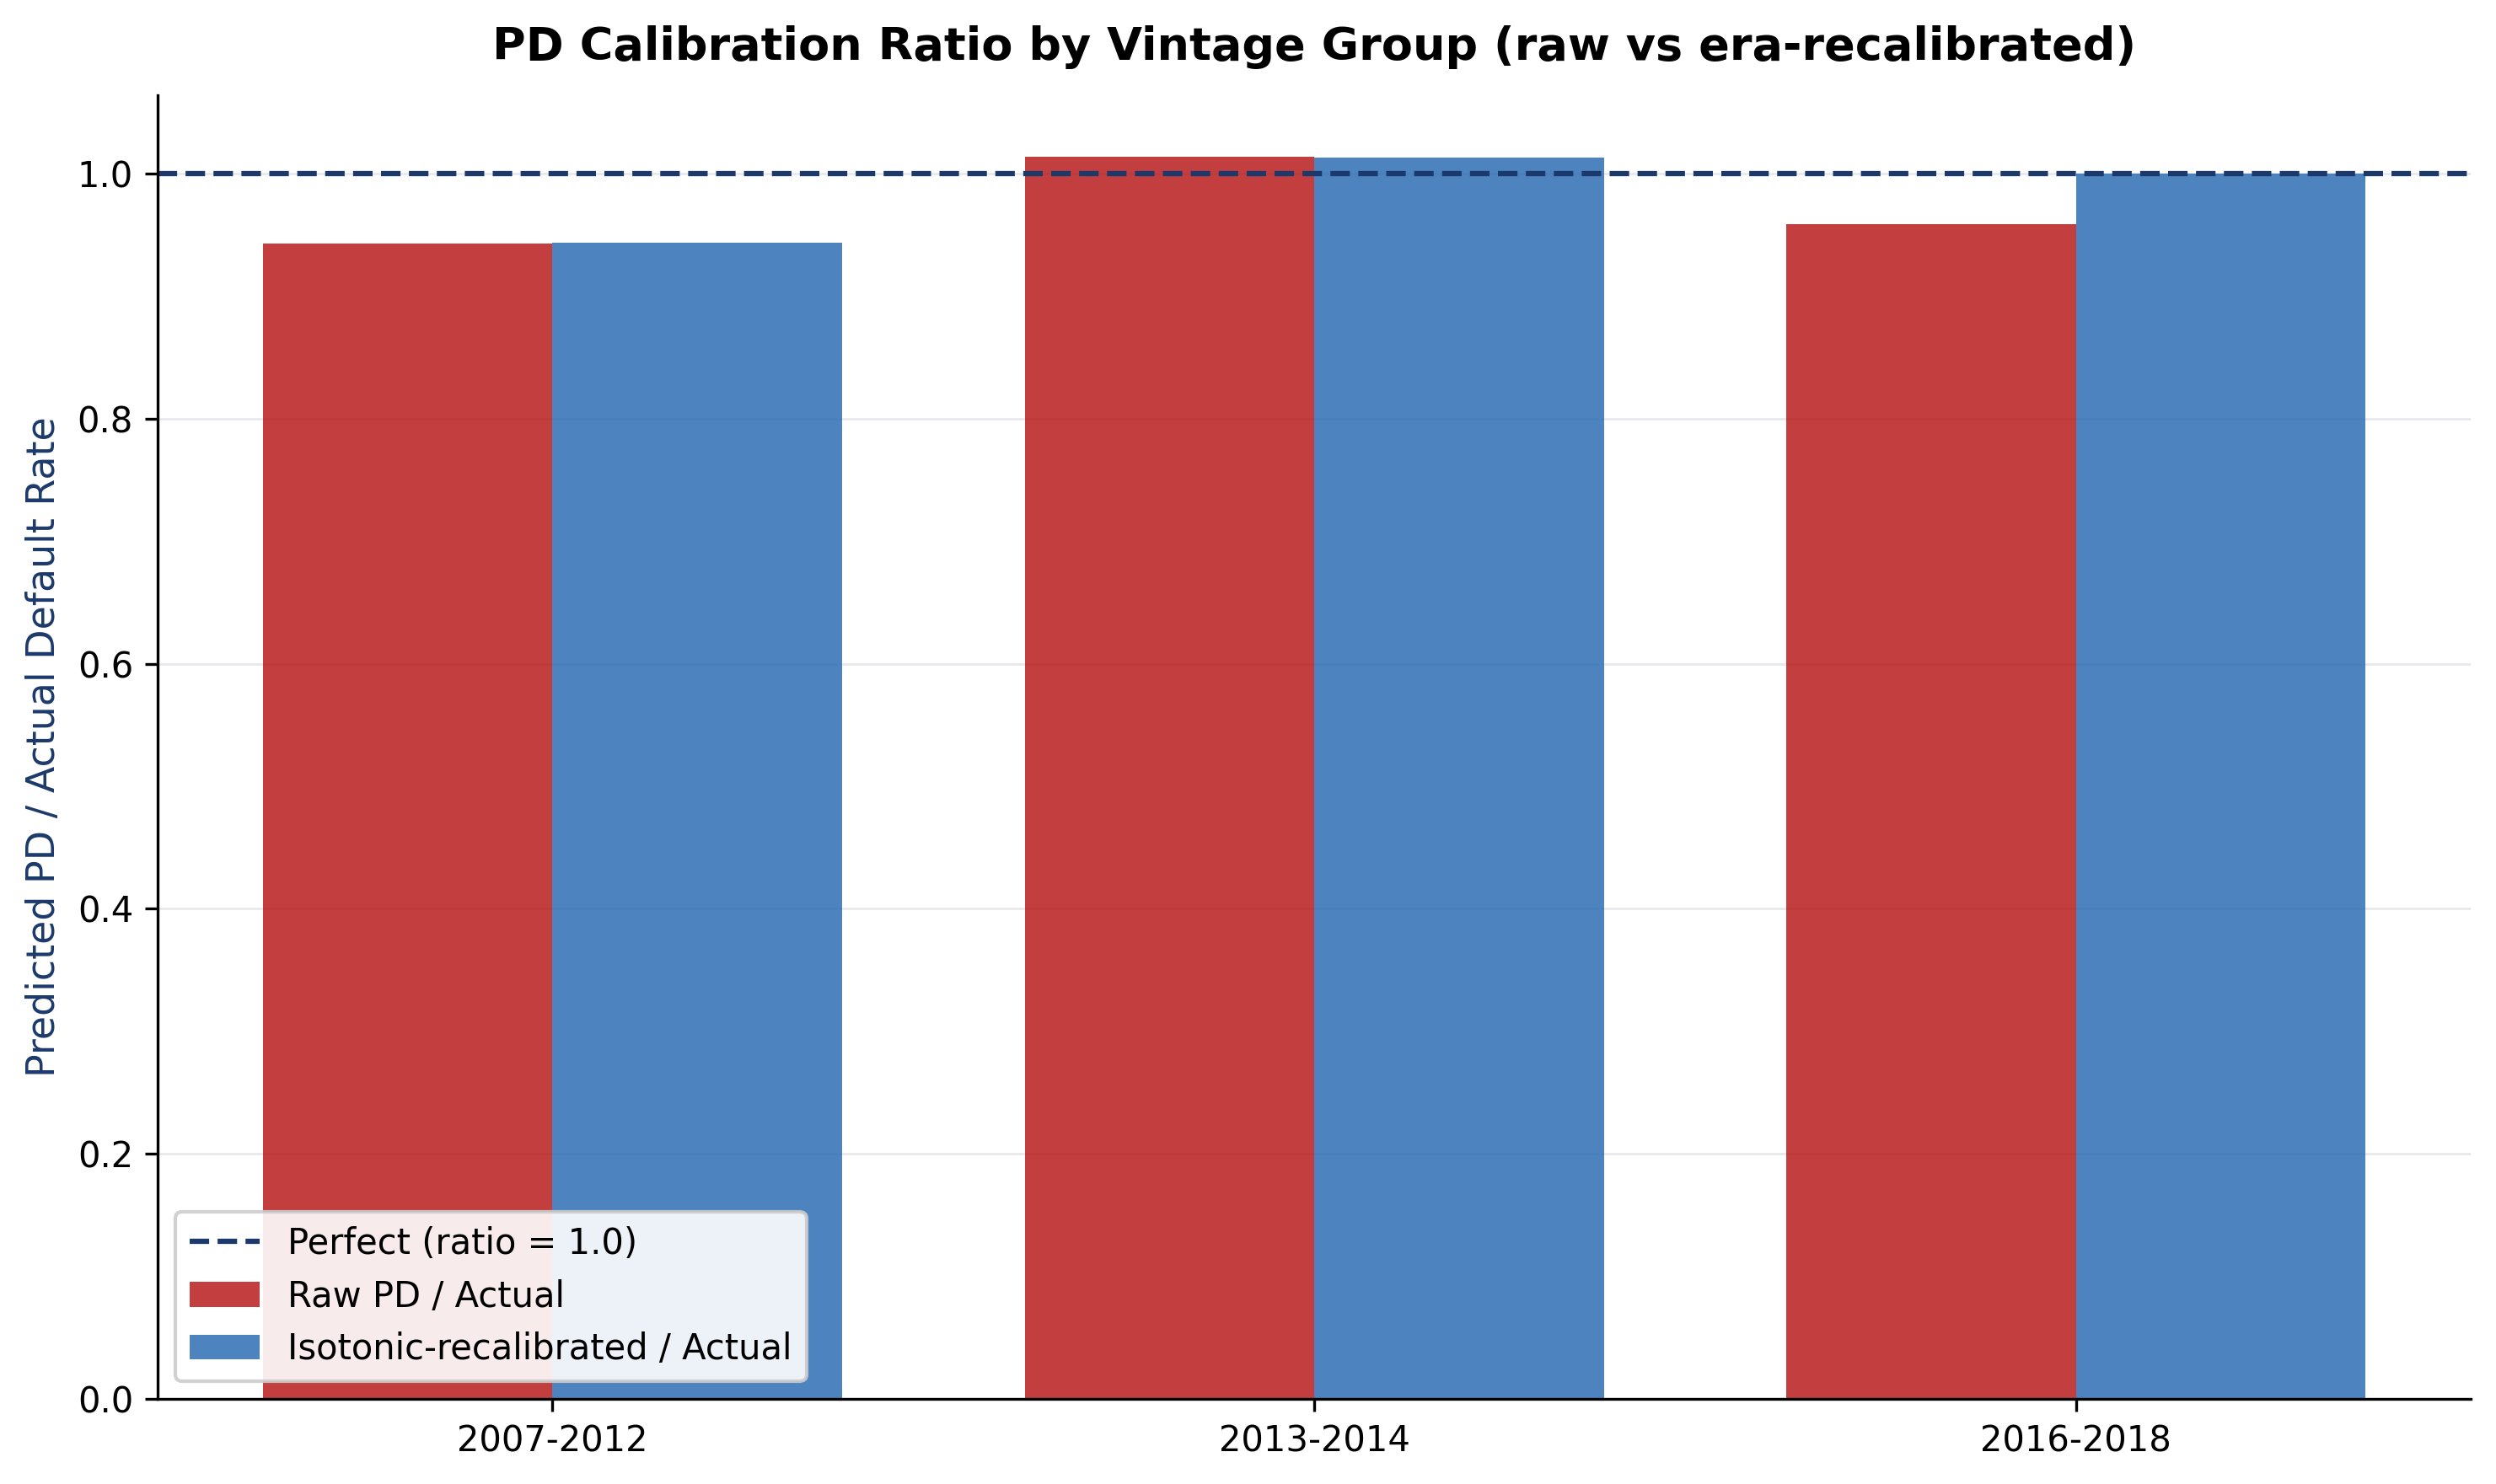
\includegraphics[width=0.65\textwidth]{figures/validation/calibration_by_vintage.png}
\caption{PD calibration ratio (predicted / actual) by vintage group, raw vs era-recalibrated. A ratio of 1.0 is perfect calibration; below 1.0 is under-prediction.}
\label{fig:vintage_calib}
\end{figure}

\subsection{Stage Migration: Why No Matrix Is Reported}

A stage migration matrix --- transitions between IFRS~9 stages from twelve months before the reporting date to the reporting date \parencite{novotny2016} --- is a standard indicator of portfolio deterioration velocity, and its absence here is deliberate.

Producing one requires the stage a loan occupied at a \emph{past} date. That requires a monthly servicing panel: balances, delinquency status and staging decisions recorded as they stood. This dataset carries no such panel. It provides one row per loan describing its state at origination and its terminal resolved outcome, with nothing in between. Two consequences follow and neither is fixable by modelling. The $t-12$ Stage~3 population is unidentifiable, because the credit-impaired flag available here \emph{is} the terminal outcome and cannot be evaluated at an earlier date --- so every row of a reconstructed matrix would be forced into Stage~1 or Stage~2. And the $t-12$ credit profile itself would have to be imputed from the same origination covariates that produce the reporting-date profile, making the resulting ``migration'' a deterministic re-labelling of the current state rather than an observed transition.

An earlier version of this report presented such a reconstructed matrix. Its cells were arithmetic artefacts of the reconstruction --- most visibly, it showed more cures than deteriorations on a book whose default rate was rising. Publishing a table that looks like observed migration but is not is worse than publishing none, so it has been withdrawn. Section~10 lists the servicing panel as the single data acquisition that would most improve this model; recording origination-date PD snapshots at booking (Section~10.2) would make a genuine matrix available from the next reporting cycle onward.

\subsection{ECL Macro Scenario Sensitivity}

Figure~\ref{fig:ecl_tornado} presents the portfolio ECL sensitivity to the Vasicek systematic factor~$Z$ across a range of macro scenarios, from severe expansion ($Z = +2.0$) to severe recession ($Z = -2.0$). This analysis follows the probability-weighted scenario methodology mandated by IFRS~9 paragraph B5.5.42 \parencite{iasb2014} and the stress testing framework of \parencite{bellini2019}.

Two things about the scale of those percentages. The reference row is $Z = 0$, the \emph{unconditional} anchor --- not the priced Baseline scenario, which carries its own non-zero implied $Z$ of \textbf{-0.1915}, and not the probability-weighted headline provision. And the denominator is the whole ECL, which is dominated by the Stage~3 term where $PD$ is forced to $1.0$ and no macro factor can reach it (Section~10.3 measures that share at \textbf{80\%} of the provision). A $\pm$22.8\% swing on the total therefore corresponds to a materially larger swing on the PD-sensitive part of the book: scaled onto the PD-sensitive remainder it is $\pm$115.6\%. Read the tornado as a sensitivity of the reported provision, not of the modelled credit risk.

\subsection{ECL What-If Calculator: PD / LGD / EAD Stress Scenarios}
Beyond the macro-factor mapping, a management-facing what-if calculator answers the direct risk-committee question \emph{``what happens to provisions if PD, LGD or EAD move?''}. Holding the baseline term structure fixed, each scenario applies a multiplicative PD shock, an additive LGD shock and/or a multiplicative EAD (drawdown) shock, and the ECL engine is re-run. Table~\ref{tab:ecl_whatif} reports the resulting provision changes, and Figure~\ref{fig:ecl_shock_tornado} presents them as a tornado chart, including regulator-style severe scenarios calibrated to COVID-19 and Global-Financial-Crisis default multiples. The anchor for these what-if sensitivities is the ECL evaluated at $Z = 0$: neither the priced Baseline scenario, which carries its own non-zero implied $Z$, nor the probability-weighted total, which additionally weights the downside and upside scenarios. That is why it differs from the headline ECL. Every entry in the table is a ratio to that same anchor, so the choice cancels.

\begin{table}[H]
\centering
\caption{ECL What-If Sensitivity (anchor ECL $=$ \$1,301.9M at $Z=0$; this is neither the priced Baseline scenario, which carries its own non-zero implied $Z$, nor the probability-weighted total ECL of Table~\ref{tab:exec_summary}, which additionally weights the Upside and Downside scenarios. Every figure below is a ratio to this same anchor, so the choice of anchor cancels)}
\label{tab:ecl_whatif}
\vspace{0.5em}
\begin{tabular}{lrrr}
\toprule
\textbf{Scenario} & \textbf{Shocked ECL (\$M)} & \textbf{$\Delta$ ECL (\$M)} & \textbf{$\Delta$ \%} \\
\midrule
PD +20\% & 1,353.57 & +51.69 & +4.0\% \\
PD +50\% & 1,430.19 & +128.31 & +9.9\% \\
LGD +10pp & 1,446.65 & +144.78 & +11.1\% \\
EAD +15\% & 1,497.16 & +195.28 & +15.0\% \\
Combined & 1,602.62 & +300.74 & +23.1\% \\
COVID-like (PD x2.5) & 1,865.66 & +563.78 & +43.3\% \\
GFC-like (PD x3.0) & 1,972.67 & +670.79 & +51.5\% \\
\bottomrule
\end{tabular}
\end{table}

\begin{figure}[H]
\centering
\begin{subfigure}[b]{0.49\textwidth}
    \centering
    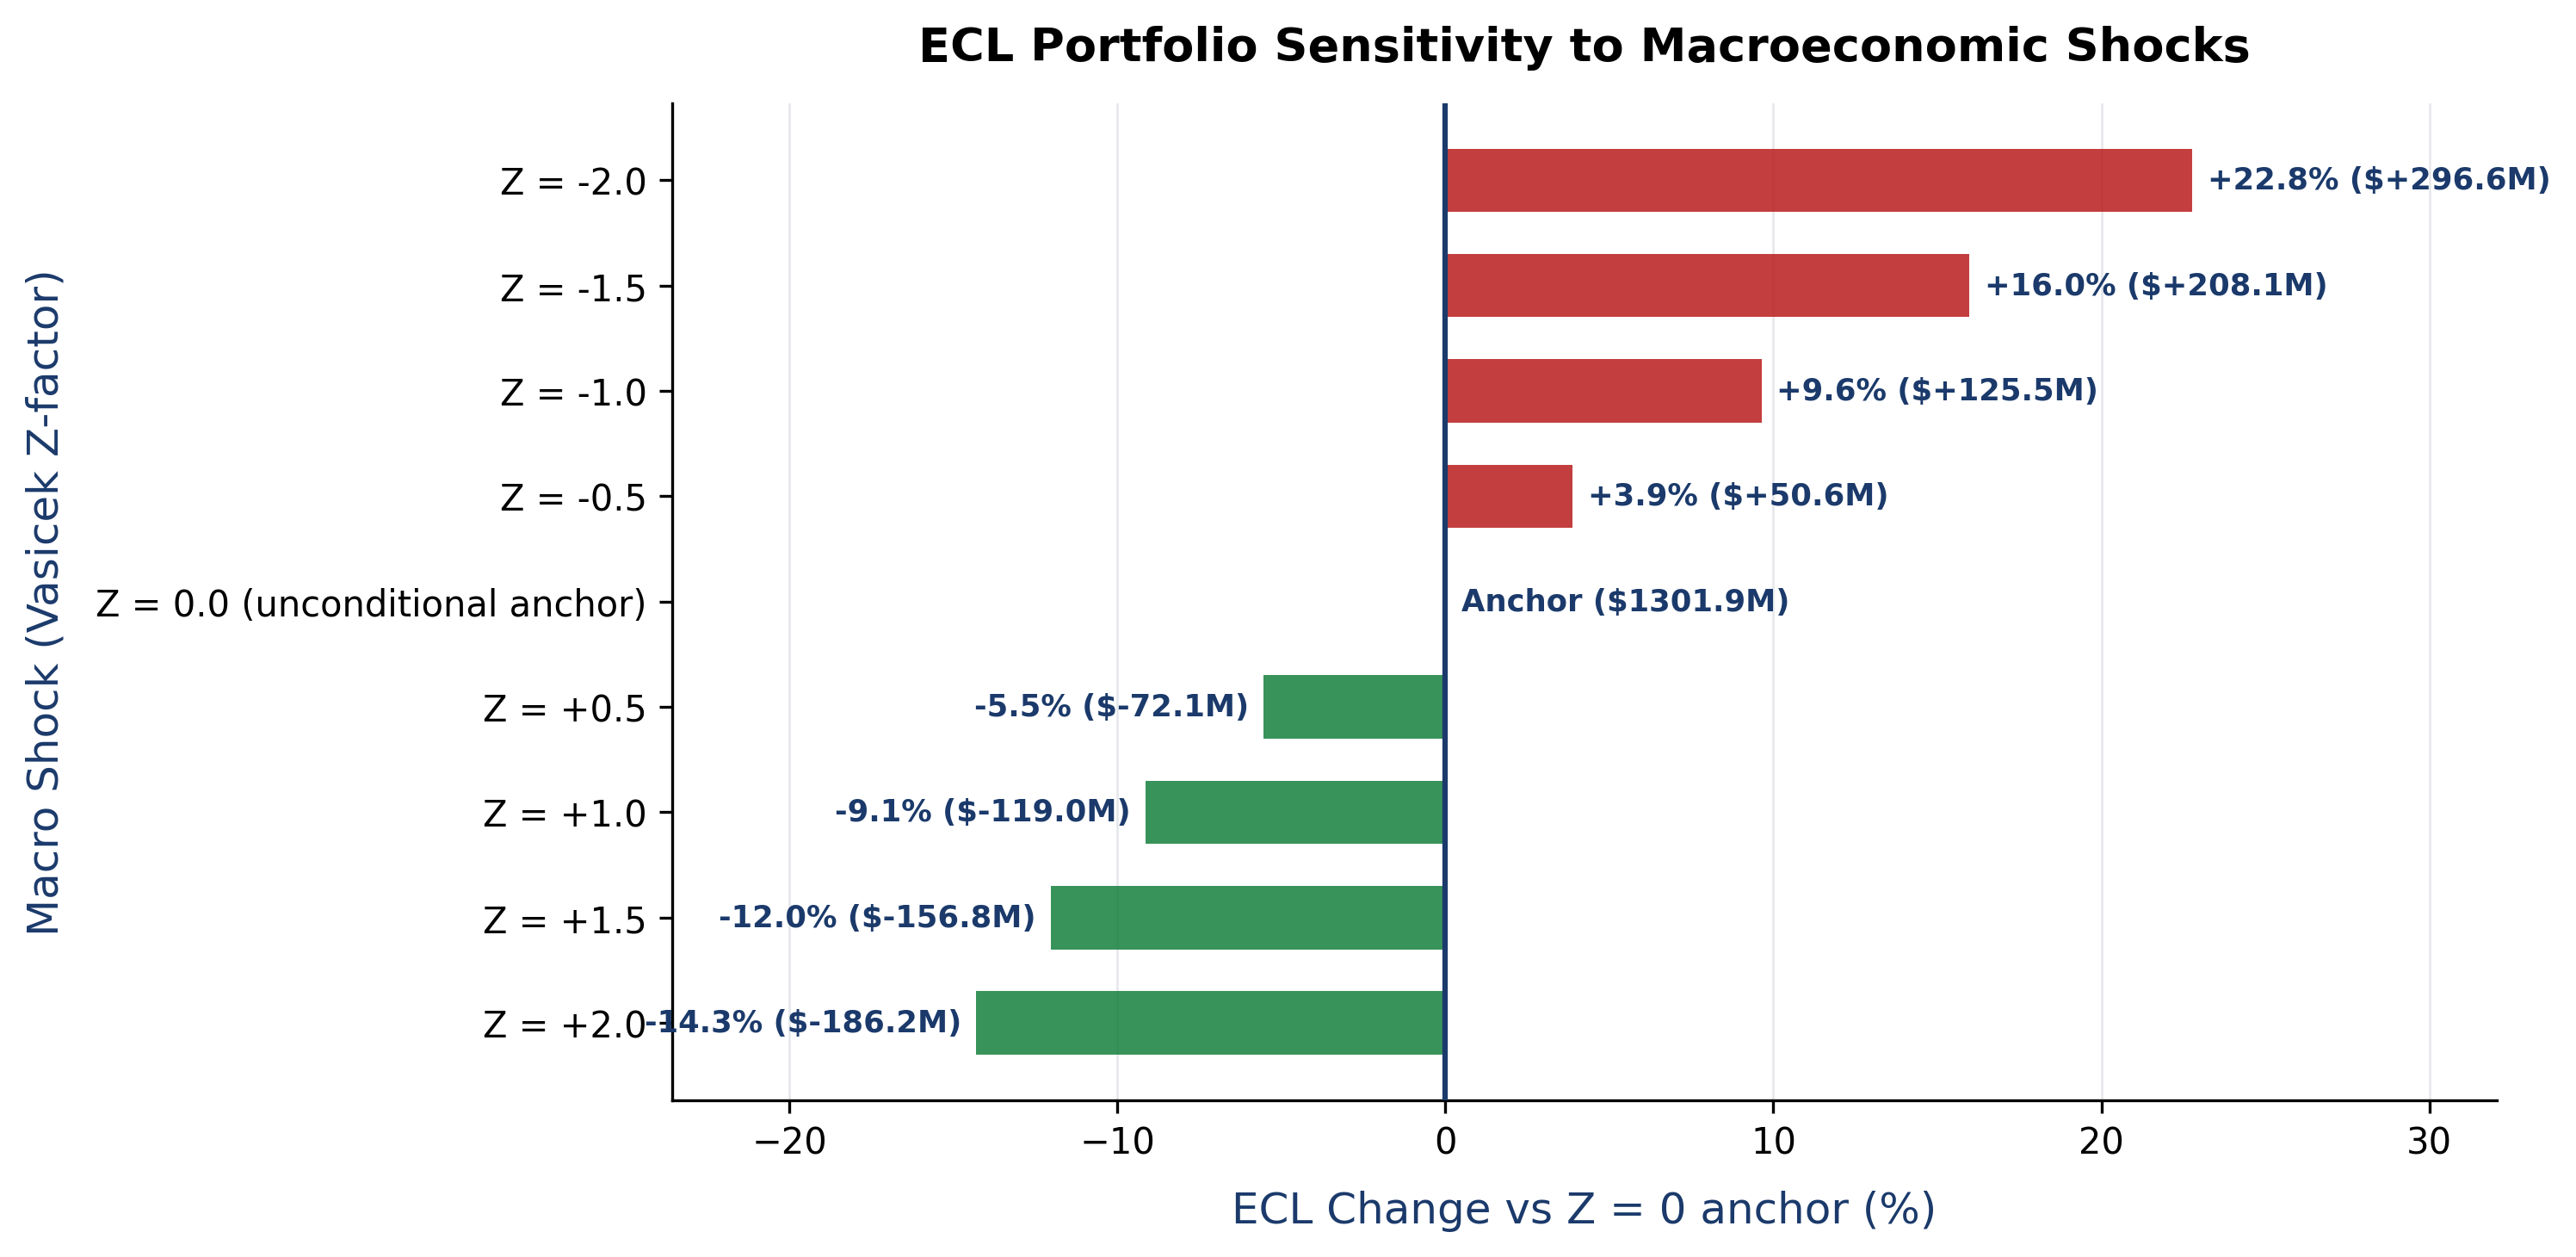
\includegraphics[width=\textwidth]{figures/ecl_tornado.png}
    \caption{Macro Sensitivity (Vasicek $Z$-Factor Shock)}
    \label{fig:ecl_tornado}
\end{subfigure}
\hfill
\begin{subfigure}[b]{0.49\textwidth}
    \centering
    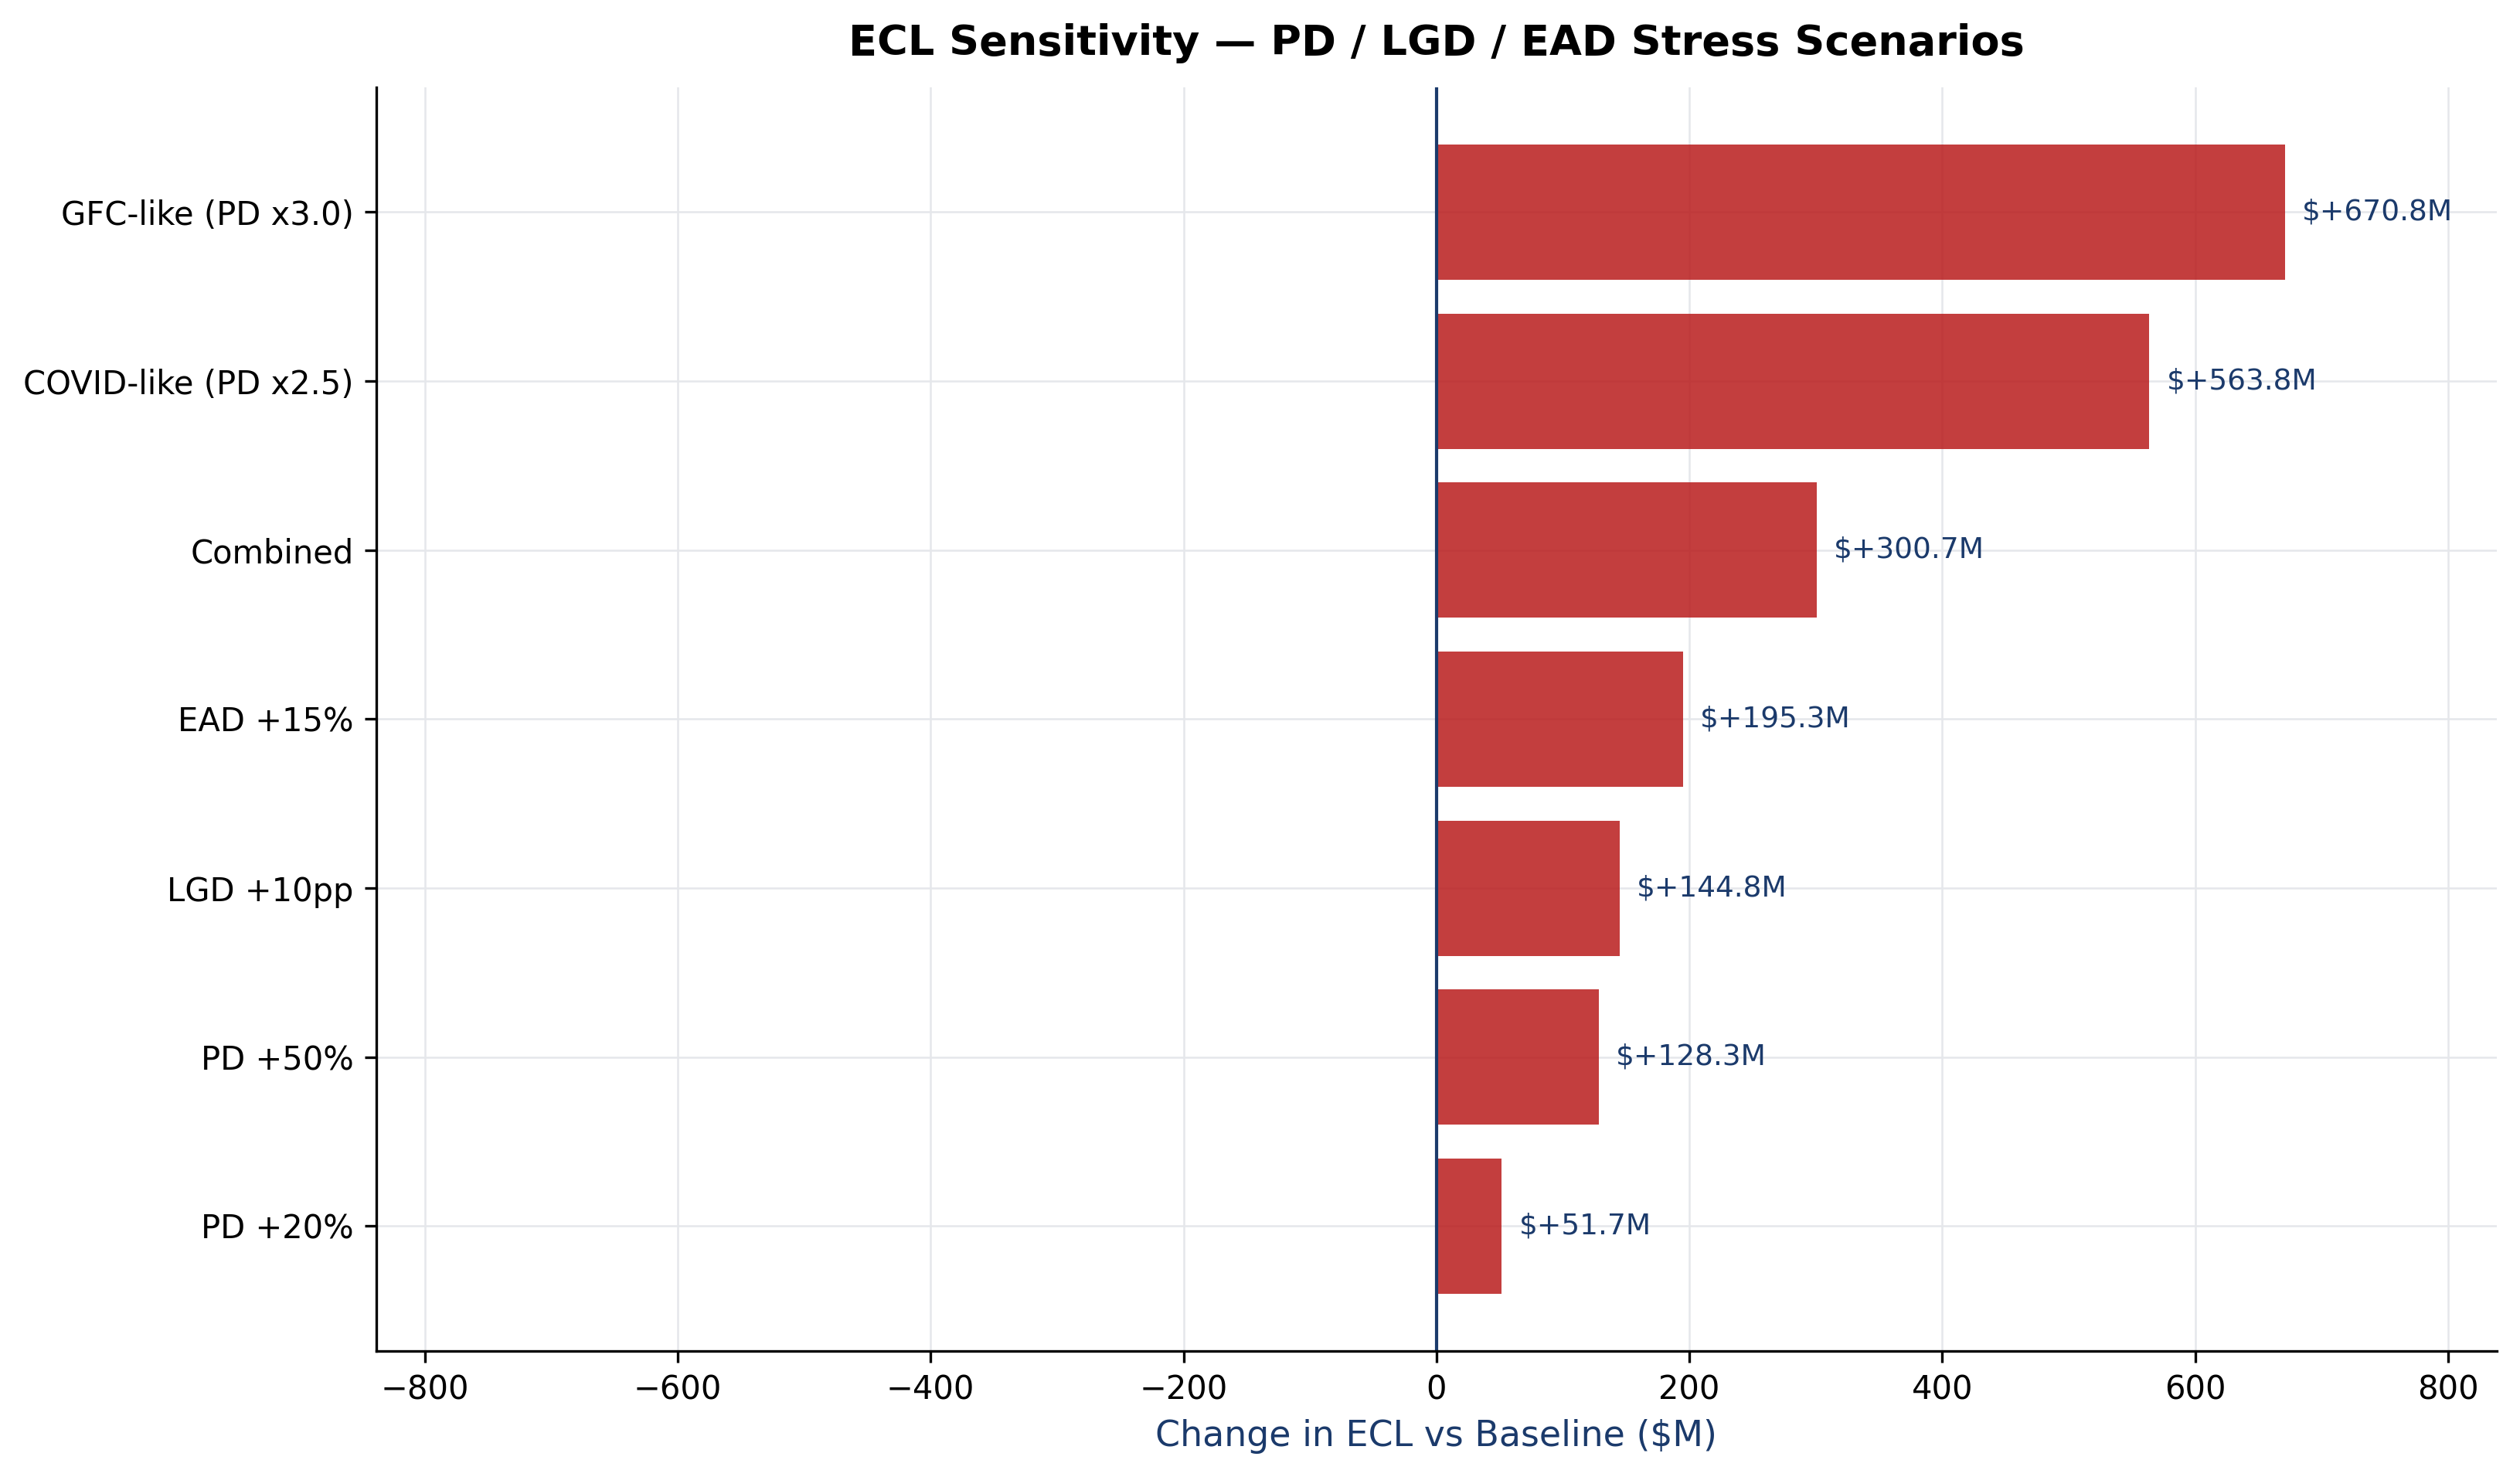
\includegraphics[width=\textwidth]{figures/ecl_shock_tornado.png}
    \caption{PD / LGD / EAD Stress Scenarios}
    \label{fig:ecl_shock_tornado}
\end{subfigure}
\caption{ECL sensitivity tornado charts (change in ECL vs baseline).}
\label{fig:ecl_tornado_combined}
\end{figure}

\subsection{Scientific Benchmark Verification Layer}

To situate our results, all modeling outputs are compared against published reference ranges drawn from the credit-risk literature. This is a comparison against published ranges, not a reproduction of the cited studies' experiments. Following \textcite{thomas2000survey} and the benchmarking study of \textcite{lessmann2015benchmarking}, our Probability of Default (PD) scorecard achieves an OOT Gini coefficient of \textbf{\num{0.4007}} (AUC of \textbf{\num{0.7003}}), which sits within the empirical range of $0.30$--$0.45$ reported for high-volume retail loan portfolios (equivalently AUC $0.65$--$0.73$, since $\text{Gini} = 2\,\text{AUC}-1$).

The deployed severity model, selected by lower out-of-sample error from a two-stage model and a LightGBM challenger, yields a Mean LGD of \textbf{\num{0.8931}} (and Downturn LGD of \textbf{\num{1.0000}}). This out-of-sample-validated loss rate sits above both the $0.45$--$0.55$ unsecured range reported by \textcite{schuermann2004} (corporate/wholesale debt) and the lower $0.25$--$0.45$ revolving retail credit-card band of \textcite{bellotti2012}, consistent with the low post-charge-off collection recovery typical of unsecured instalment loans once EAD is measured on a principal-only basis (driver discussed in Table~\ref{tab:benchmark_verification}).

Under the Basel Committee regulatory standards \parencite{bcbs2004,bcbs2017}, the risk-sensitive internal ratings-based (IRB) approach sets our Risk-Weighted Asset (RWA) density at \textbf{161.7\%}, above the flat 75\% risk weight assumed by the Standardised Approach (SA). Because this portfolio is a high-yield, higher-risk unsecured book, the risk-sensitive approach produces a capital \emph{surcharge} rather than relief, the expected outcome when portfolio risk exceeds the level implicit in the flat SA weight.

Consistent with the reject inference analysis of \textcite{crook2004reject}, the inclusion of parcelled rejected applications leads to a Gini shift of \textbf{\num{-0.0656}}. This shift is consistent with the presence of selection bias; through-the-door refitting produces a small, conservative change in the fitted parameters.

Table~\ref{tab:benchmark_verification} presents a structured side-by-side comparison of our empirical results against published scientific benchmarks.

\begin{table}[H]
\centering
\footnotesize
\setlength{\tabcolsep}{2.5pt}
\caption{Comparison against published reference ranges. Verdicts are computed numerically at build time by comparing the Project Value column against the published range; each range is sourced from a single registry (reports/benchmarks.py) with its citation. These are literature reference ranges, not a reproduction of the cited studies.}
\label{tab:benchmark_verification}
\vspace{0.5em}
\begin{tabularx}{\linewidth}{p{2.2cm}ccp{2.2cm}cp{4.5cm}}
\toprule
\textbf{Metric / Parameter} & \textbf{Project Value} & \textbf{Published Benchmark} & \textbf{Academic Source} & \textbf{Verdict} & \textbf{Comment} \\
\midrule
PD AUC (OOT) & \textbf{\num{0.7003}} & $0.65 - 0.73$ & \textcite{lessmann2015benchmarking} & Within range &  \\
PD Gini (OOT) & \textbf{\num{0.4007}} & $0.30 - 0.45$ & \textcite{lessmann2015benchmarking} & Within range & \\
LGD Mean & \textbf{\num{0.8931}} & $0.25 - 0.45$ & \textcite{bellotti2012} & Above typical range & The OOS-validated LightGBM severity model puts mean LGD above both cited bands, consistent with low post-charge-off recovery on unsecured instalment loans once EAD is principal-only; the rejected two-stage model materially under-predicted severity (OOS $R^2 \approx -2.70$) \\
LGD $R^2$ (OOS) & \textbf{-0.0709} & $0.04 - 0.43$ & \textcite{loterman2012benchmarking} & Below typical range & LGD is strongly bimodal (mass at 0 and near 1), so $R^2$ is an unforgiving metric and is routinely low or negative out-of-time; \textcite{loterman2012benchmarking} themselves report a wide $0.04$--$0.43$ spread. The negative value reflects a 2016--2018 severity regime shift versus the fitting vintages \\
RWA Density & \textbf{161.7\%} & 75\% -- 100\% & \textcite{bcbs2017} & Above typical range & Risk-sensitive IRB density exceeds the flat SA weight: the OOS-validated LGD (mean $\approx 0.89$, above published unsecured LGD ranges --- driver discussed in the LGD Mean row above) and high empirical default rate on this unsecured, high-yield book drive a capital \emph{surcharge} --- the economically expected outcome, not an inconsistency \\
IRB vs SA Capital & IRB $>$ SA & Risk-sensitive & \textcite{bcbs2004} & Consistent & Risk-sensitive IRB exceeds the flat 75\% SA weight for this higher-risk unsecured book: a capital \emph{surcharge}, not relief, is the economically expected outcome \\
Reject Inference $\Delta$Gini & \textbf{\num{-0.0656}} & $0.00 - 0.10$ & \textcite{crook2004reject} & Below typical range & \\
Score PSI & \textbf{\num{0.0032}} & $0.00 - 0.10$ & \textcite{siddiqi2017} & Within range & \\
\bottomrule
\end{tabularx}
\end{table}

\subsection{Machine Learning Champion-Challenger Benchmarking}

To evaluate whether the linear scorecard loses significant predictive power compared to non-linear alternatives, we constructed a Champion-Challenger benchmarking layer. We trained and evaluated:
\begin{enumerate}
    \item \textbf{Logistic Scorecard:} Our baseline WoE scorecard.
    \item \textbf{LightGBM Classifier:} A state-of-the-art tree boosting model.
    \item \textbf{XGBoost Classifier:} A highly optimized distributed gradient boosting model.
    \item \textbf{Random Forest Classifier:} A classic tree-bagging model.
    \item \textbf{Weighted Ensemble:} A weighted combination of scorecard ($30\%$), LightGBM ($30\%$), XGBoost ($20\%$), and Random Forest ($20\%$).
\end{enumerate}

Table~\ref{tab:ml_comparison} presents the out-of-time (OOT) generalization benchmarks, discrimination statistics (AUC, Gini, KS), and computational costs for each algorithm.

\begin{table}[H]
\centering
\small
\setlength{\tabcolsep}{3.2pt}
\caption{Machine Learning Champion-Challenger Performance Comparison}
\label{tab:ml_comparison}
\vspace{0.5em}
\begin{tabular}{lccccccr}
\toprule
\textbf{Model Name} & \textbf{Test AUC} & \textbf{OOT AUC} & \textbf{Test Gini} & \textbf{OOT Gini} & \textbf{Test KS} & \textbf{OOT KS} & \textbf{Time (s)} \\
\midrule
\textbf{Logistic Scorecard} & 0.7020 & 0.7003 & 0.4041 & 0.4007 & 0.2935 & 0.2894 & 197.20s \\
\textbf{LightGBM Classifier} & 0.7064 & 0.7033 & 0.4128 & 0.4067 & 0.3026 & 0.2934 & 2.65s \\
\textbf{XGBoost Classifier} & 0.7065 & 0.7027 & 0.4130 & 0.4054 & 0.3005 & 0.2930 & 4.71s \\
\textbf{Random Forest Classifier} & 0.7041 & 0.7006 & 0.4082 & 0.4013 & 0.2971 & 0.2891 & 12.62s \\
\textbf{Weighted Ensemble} & 0.7065 & 0.7037 & 0.4130 & 0.4074 & 0.3020 & 0.2941 & 19.98s \\
\bottomrule
\end{tabular}
\end{table}

Notably, the tree-based challengers, evaluated on an identical predictor set, \emph{outperform} the WoE logistic scorecard on out-of-time discrimination: the scorecard's OOT AUC of 0.7003 is exceeded by Weighted Ensemble (0.7037), LightGBM Classifier (0.7033), XGBoost Classifier (0.7027), Random Forest Classifier (0.7006). The best challenger (Weighted Ensemble) leads by 0.0034 AUC. We report this plainly rather than presenting the scorecard as the discrimination winner: it is not. The scorecard is retained as champion on \emph{governance} grounds --- exact per-feature points attribution for adverse-action reasons, a monotone and auditable functional form, and a stable calibration story --- and the cost of that choice is the AUC gap quantified here, which a model-risk committee should weigh explicitly rather than have hidden. \textbf{Feature parity.} The scorecard consumes 16 selected predictors and the tree challengers consume 16; the two model families are therefore evaluated on an identical predictor set, so the comparison above is like-for-like. It should be noted that the challenger models (LightGBM, XGBoost, Random Forest) were trained using standard, default configurations without systematic hyperparameter grid search tuning. Hyperparameter optimisation would, if anything, widen any challenger advantage, so the ranking above should be read as a lower bound on what tuned tree models could achieve on this feature set.

\subsubsection*{Is the Challenger's Edge Statistically Significant?}
Point-estimate AUC/Gini gaps cannot distinguish a genuine improvement from sampling noise. To test significance we run a paired bootstrap: the same held-out OOT rows are resampled for both models and a confidence interval is built on the \emph{difference} in Gini (challenger $-$ champion). If that interval excludes zero, the difference is significant. Table~\ref{tab:ab_test} reports the result --- the interval lies entirely \emph{above} zero (median $+0.0060$), so the challenger's Gini advantage over the champion is statistically significant, not sampling noise. It complements the analytic DeLong test on the same pair, which is computed with the full covariance term of \textcite{delong1988}: both models score the same loans, so their AUC estimates are strongly positively correlated ($\rho = 0.968$ on this run) and $\mathrm{Var}(\widehat{A}_1 - \widehat{A}_2) = \mathrm{Var}(\widehat{A}_1) + \mathrm{Var}(\widehat{A}_2) - 2\,\mathrm{Cov}(\widehat{A}_1, \widehat{A}_2)$. Dropping that covariance --- as an independent-samples approximation does --- inflates the standard error and makes the test conservative by a wide margin. The same paired bootstrap is run for the \emph{Weighted Ensemble}, which is the row the champion-versus-challenger discussion in Section~3.6 refers to: its Gini advantage over the scorecard is statistically significant (95\% CI on the Gini difference: [+0.0061, +0.0073]). Note also that the ensemble is not an independent model: 30\% of its prediction is the champion scorecard itself, at weights fixed a priori rather than optimised.

\begin{table}[H]
\centering
\caption{Paired Bootstrap A/B Test --- Gini with 95\% CIs ($n_{\text{boot}}=2,000$)}
\label{tab:ab_test}
\vspace{0.5em}
\begin{tabular}{lcc}
\toprule
\textbf{Model} & \textbf{Gini (median)} & \textbf{95\% CI} \\
\midrule
Champion (Scorecard) & 0.4008 & [0.3976, 0.4036] \\
Challenger (LightGBM) & 0.4067 & [0.4037, 0.4096] \\
\midrule
Difference (B $-$ A) & 0.0060 & [0.0052, 0.0068] \\
\bottomrule
\multicolumn{3}{l}{\footnotesize Significant (CI excludes 0)} \\
\end{tabular}
\end{table}

\subsection{SHAP Explainability: Challenger Model Feature Contributions}

While the primary WoE scorecard provides point-attributable explanations per feature bin \parencite[Ch.~4]{siddiqi2017}, the LightGBM challenger model is interpreted via SHAP (SHapley Additive exPlanations) values \parencite{lundberg2017}. Figure~\ref{fig:shap} displays the mean absolute SHAP contribution of each feature: \texttt{grade\_enc} and \texttt{term\_enc} dominate the challenger's default discrimination.

\begin{figure}[H]
\centering
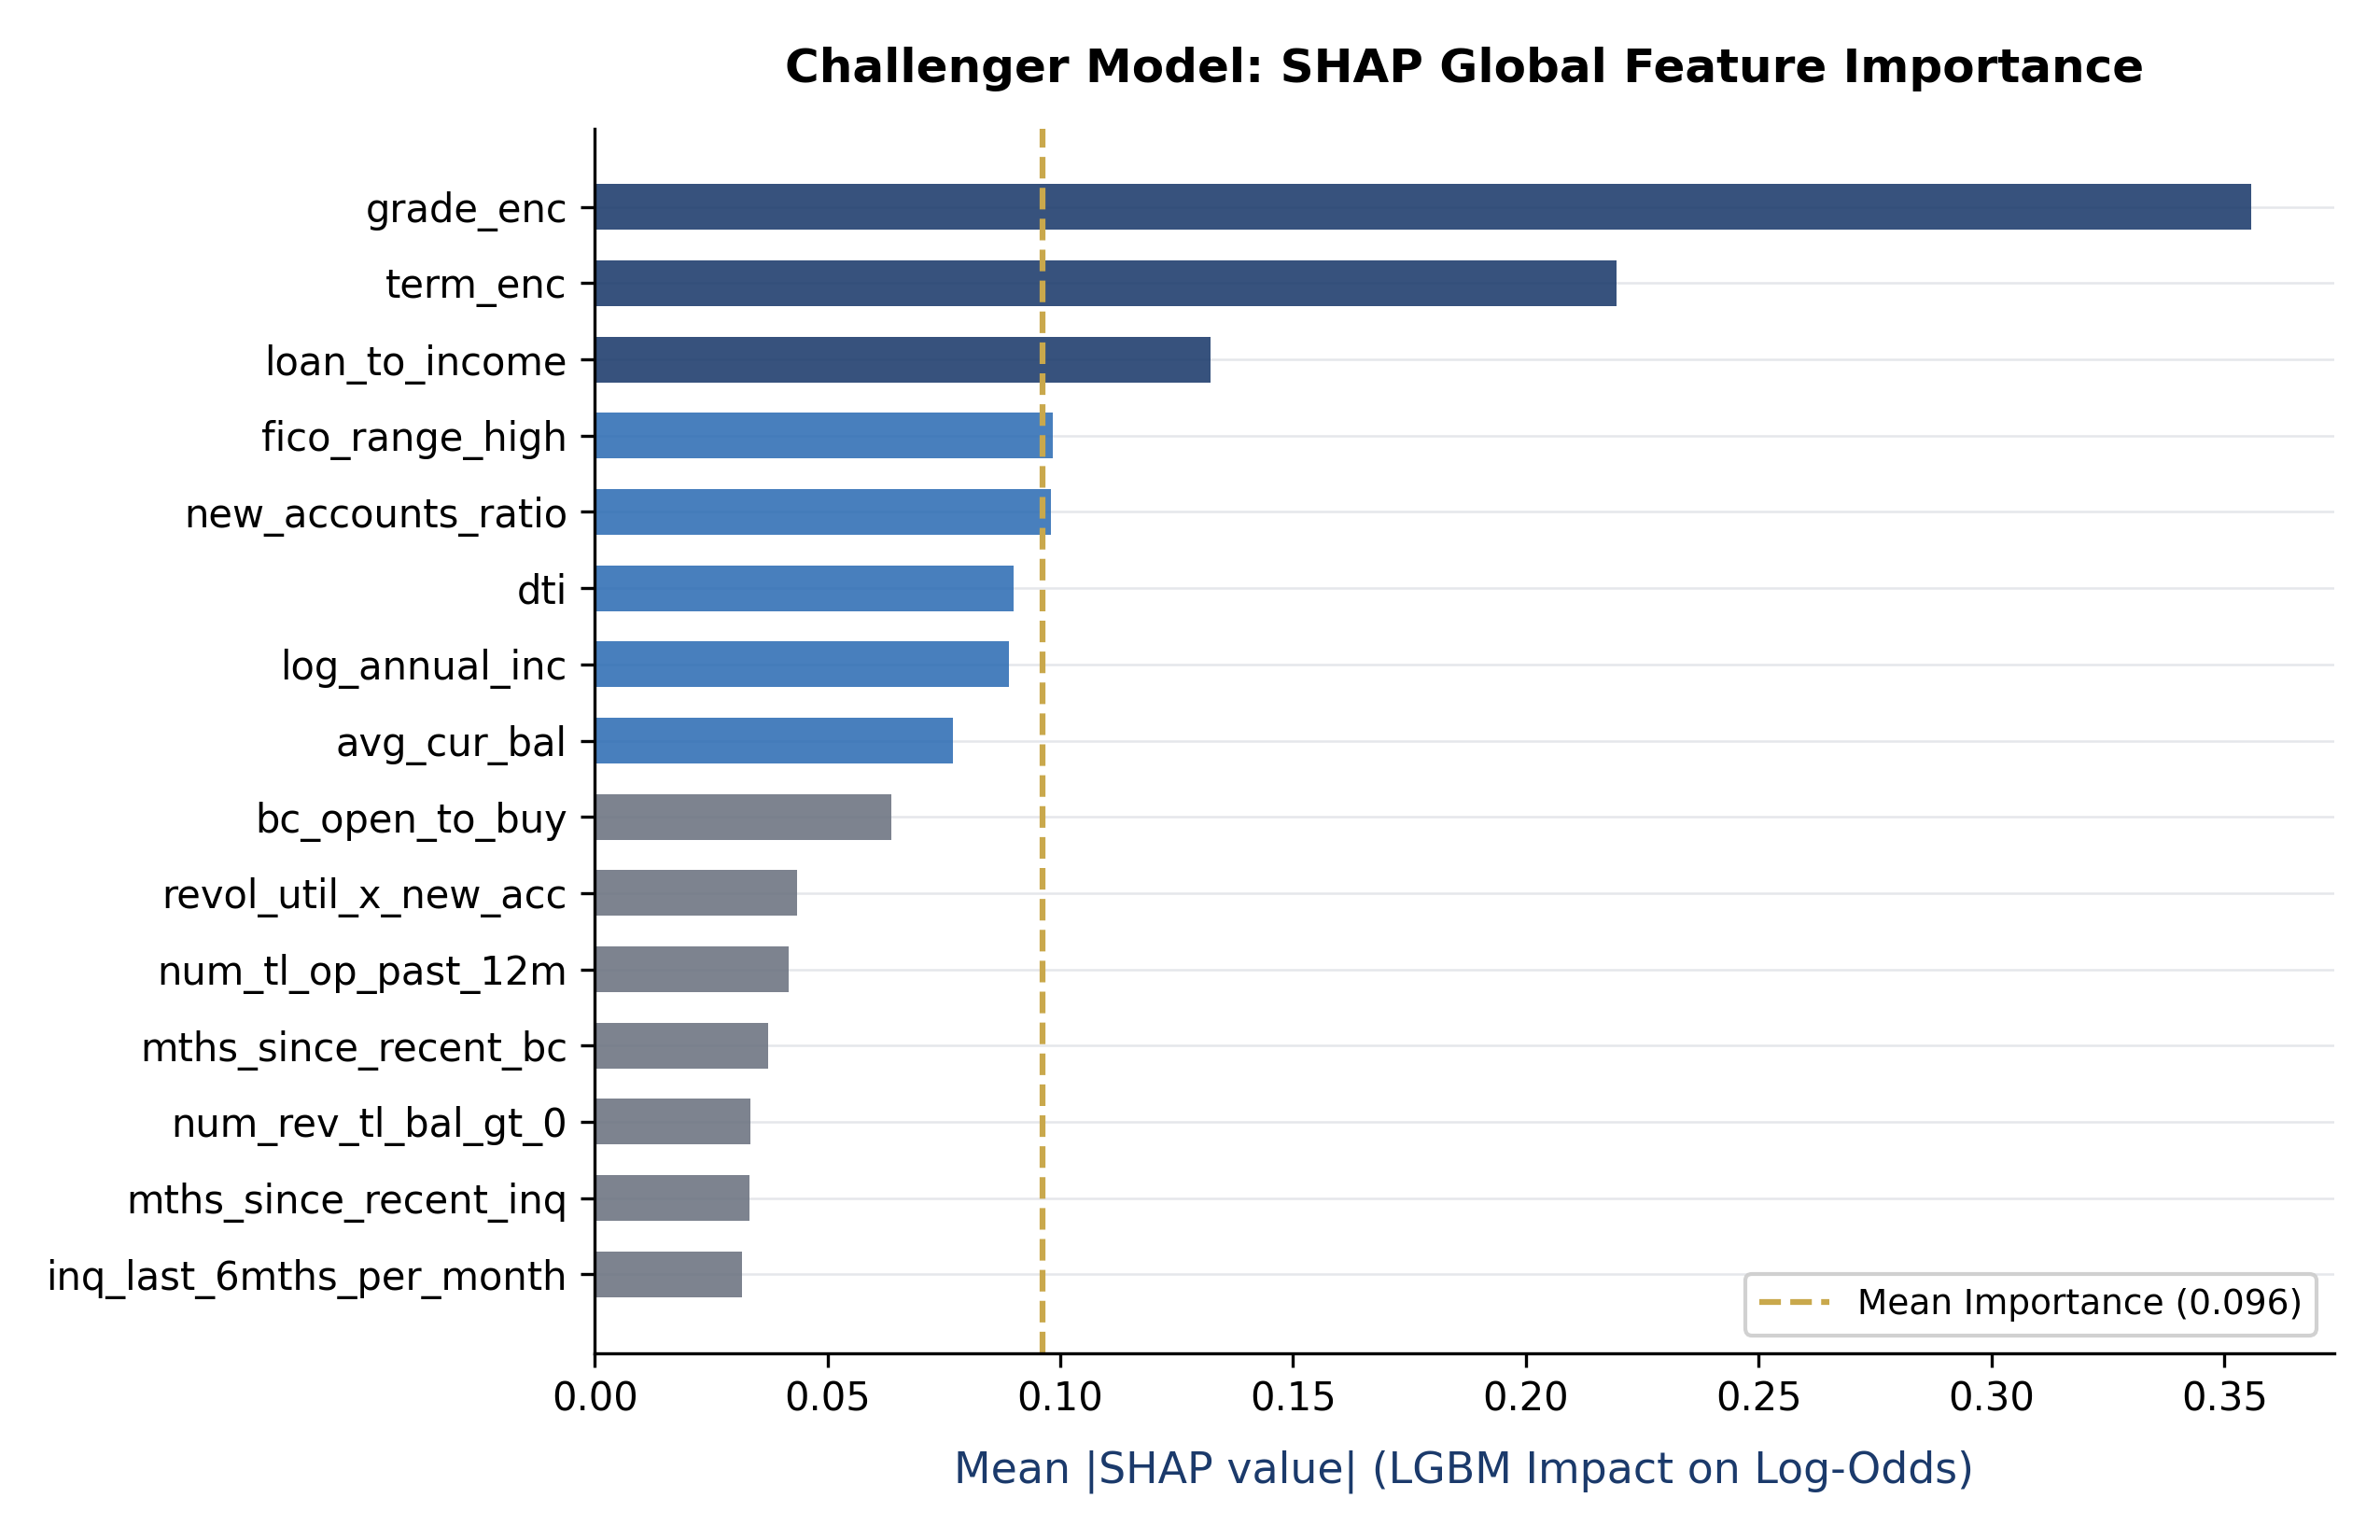
\includegraphics[width=0.64\textwidth]{figures/validation/shap_challenger_summary.png}
\caption{SHAP Feature Importance --- LightGBM Challenger Model}
\label{fig:shap}
\end{figure}

% -----------------------------------------------------------------------------
% 8. STABILITY AND PERFORMANCE OVERLAYS
% -----------------------------------------------------------------------------
\section{Stability and Performance Overlays}

\subsection{Scorecard Population Stability (PSI)}
The Population Stability Index (PSI) \parencite[Ch.~9]{engelmann2011} is computed here on the distribution of \textbf{predicted PD} --- not of credit scores --- between the training and OOT populations. Its value is \textbf{0.0032}, far below the conservative regulatory threshold of \textbf{0.10}: the shape of the model's output distribution is essentially unchanged across the two windows.

\textbf{This is not, on its own, reassurance.} Over the same interval the realised default rate rose from 17.09\% to 26.33\%. A near-zero PSI alongside a materially higher outcome rate says that the model's inputs did not move while what they were predicting did --- the scorecard did not \emph{see} the deterioration. That is precisely the calibration drift diagnosed in Sections~7.2 and~7.3, and the two findings should be read together rather than as an encouraging stability result followed by an unrelated calibration problem. PSI provides assurance only when the outcome rate is also stable; here it is not, so the per-feature Characteristic Stability Index in Table~\ref{tab:csi} is the more informative diagnostic of where (or whether) the input distributions shifted.

\begin{table}[H]
\centering
\caption{Characteristic Stability Index (CSI) by Scorecard Feature, Train vs.\ OOT}
\label{tab:csi}
\vspace{0.5em}
\small
\begin{tabular}{lcc}
\toprule
\textbf{Feature} & \textbf{CSI} & \textbf{Stability Band} \\
\midrule
\texttt{new\_accounts\_ratio} & 0.1417 & moderate\_shift \\
\texttt{bc\_open\_to\_buy} & 0.0950 & stable \\
\texttt{num\_tl\_op\_past\_12m} & 0.0451 & stable \\
\texttt{inq\_last\_6mths\_per\_month} & 0.0445 & stable \\
\texttt{num\_rev\_tl\_bal\_gt\_0} & 0.0405 & stable \\
\texttt{dti} & 0.0338 & stable \\
\texttt{mort\_acc} & 0.0296 & stable \\
\texttt{loan\_to\_income} & 0.0205 & stable \\
\bottomrule
\end{tabular}
\parbox{0.92\textwidth}{\footnotesize \vspace{0.4em} CSI is the PSI statistic applied one feature at a time. Bands follow the same convention as PSI: below 0.10 stable, 0.10--0.25 moderate shift, above 0.25 material shift. The 5 features not shown all sit below 0.0163 and are stable by this measure.}
\end{table}

\begin{figure}[H]
\centering
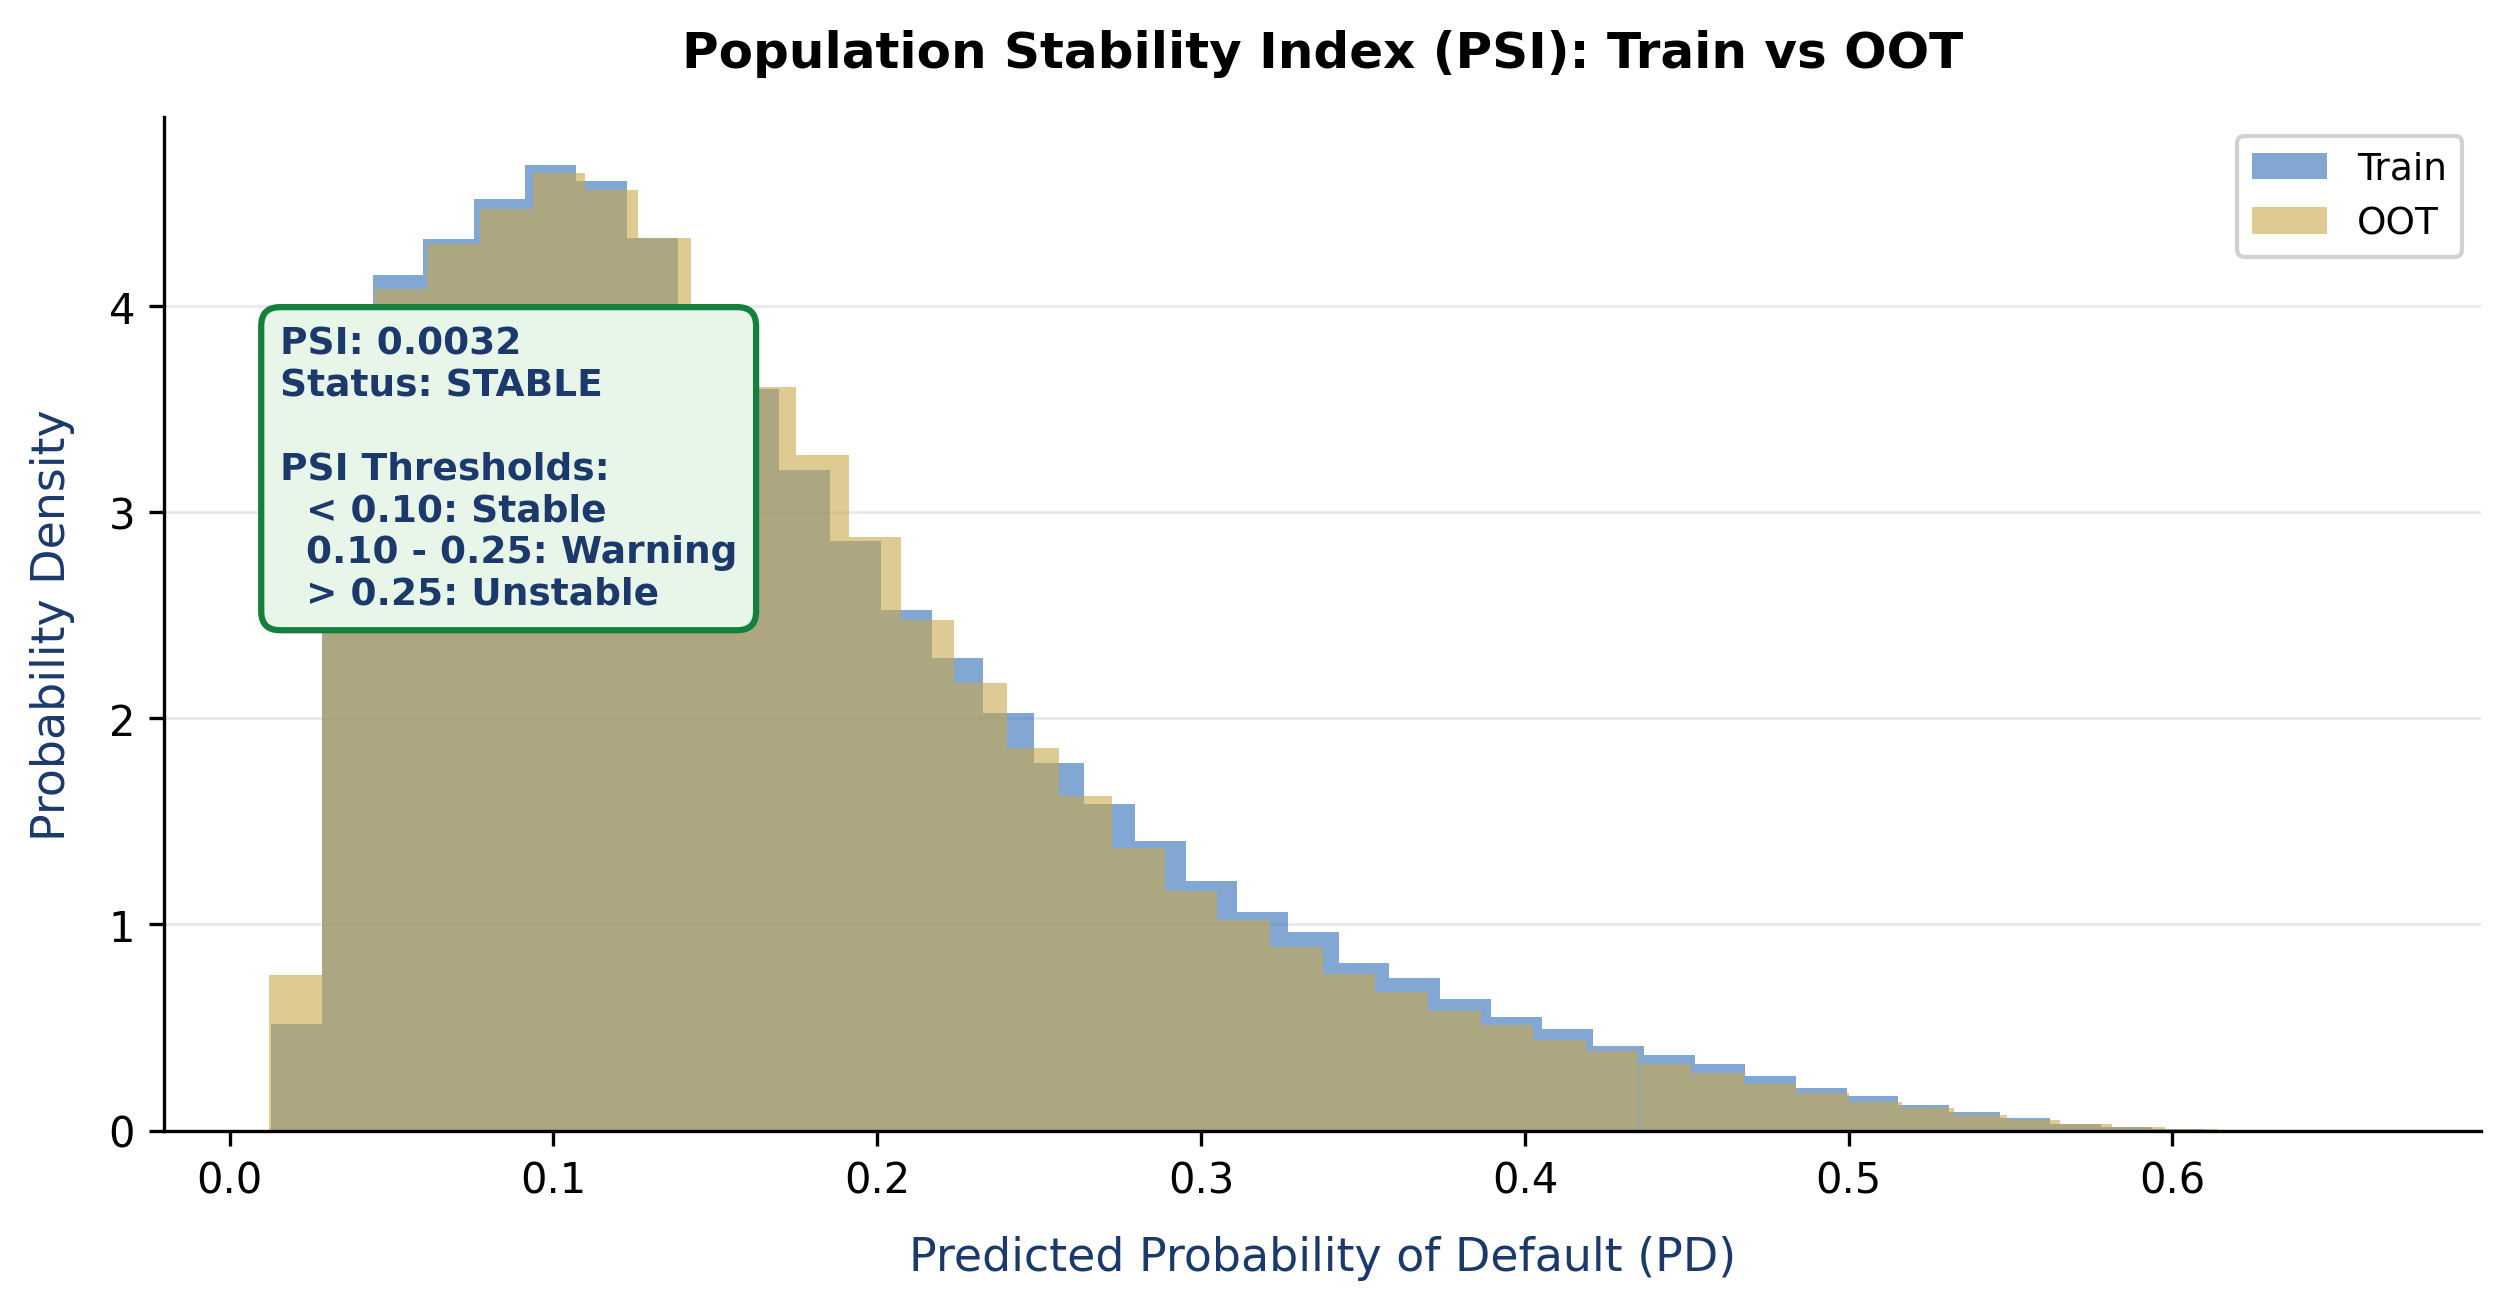
\includegraphics[width=0.64\textwidth]{figures/validation/psi_distribution.png}
\caption{Score Distribution Stability (Train vs.\ OOT)}
\label{fig:psi_dist}
\end{figure}

\subsection{Gains and Lift Analysis}
The Gains Chart measures the model's ability to concentrate defaults within the lowest score bands. The scorecard concentrates most defaults in the lowest score bands (Figure~\ref{fig:gains_ch}). Both panels below are computed on the \textbf{out-of-time} partition, so they describe generalisation rather than in-sample fit; the gains chart previously used the in-time test partition while being presented alongside OOT material.

\begin{figure}[H]
\centering
\begin{subfigure}[b]{0.49\textwidth}
    \centering
    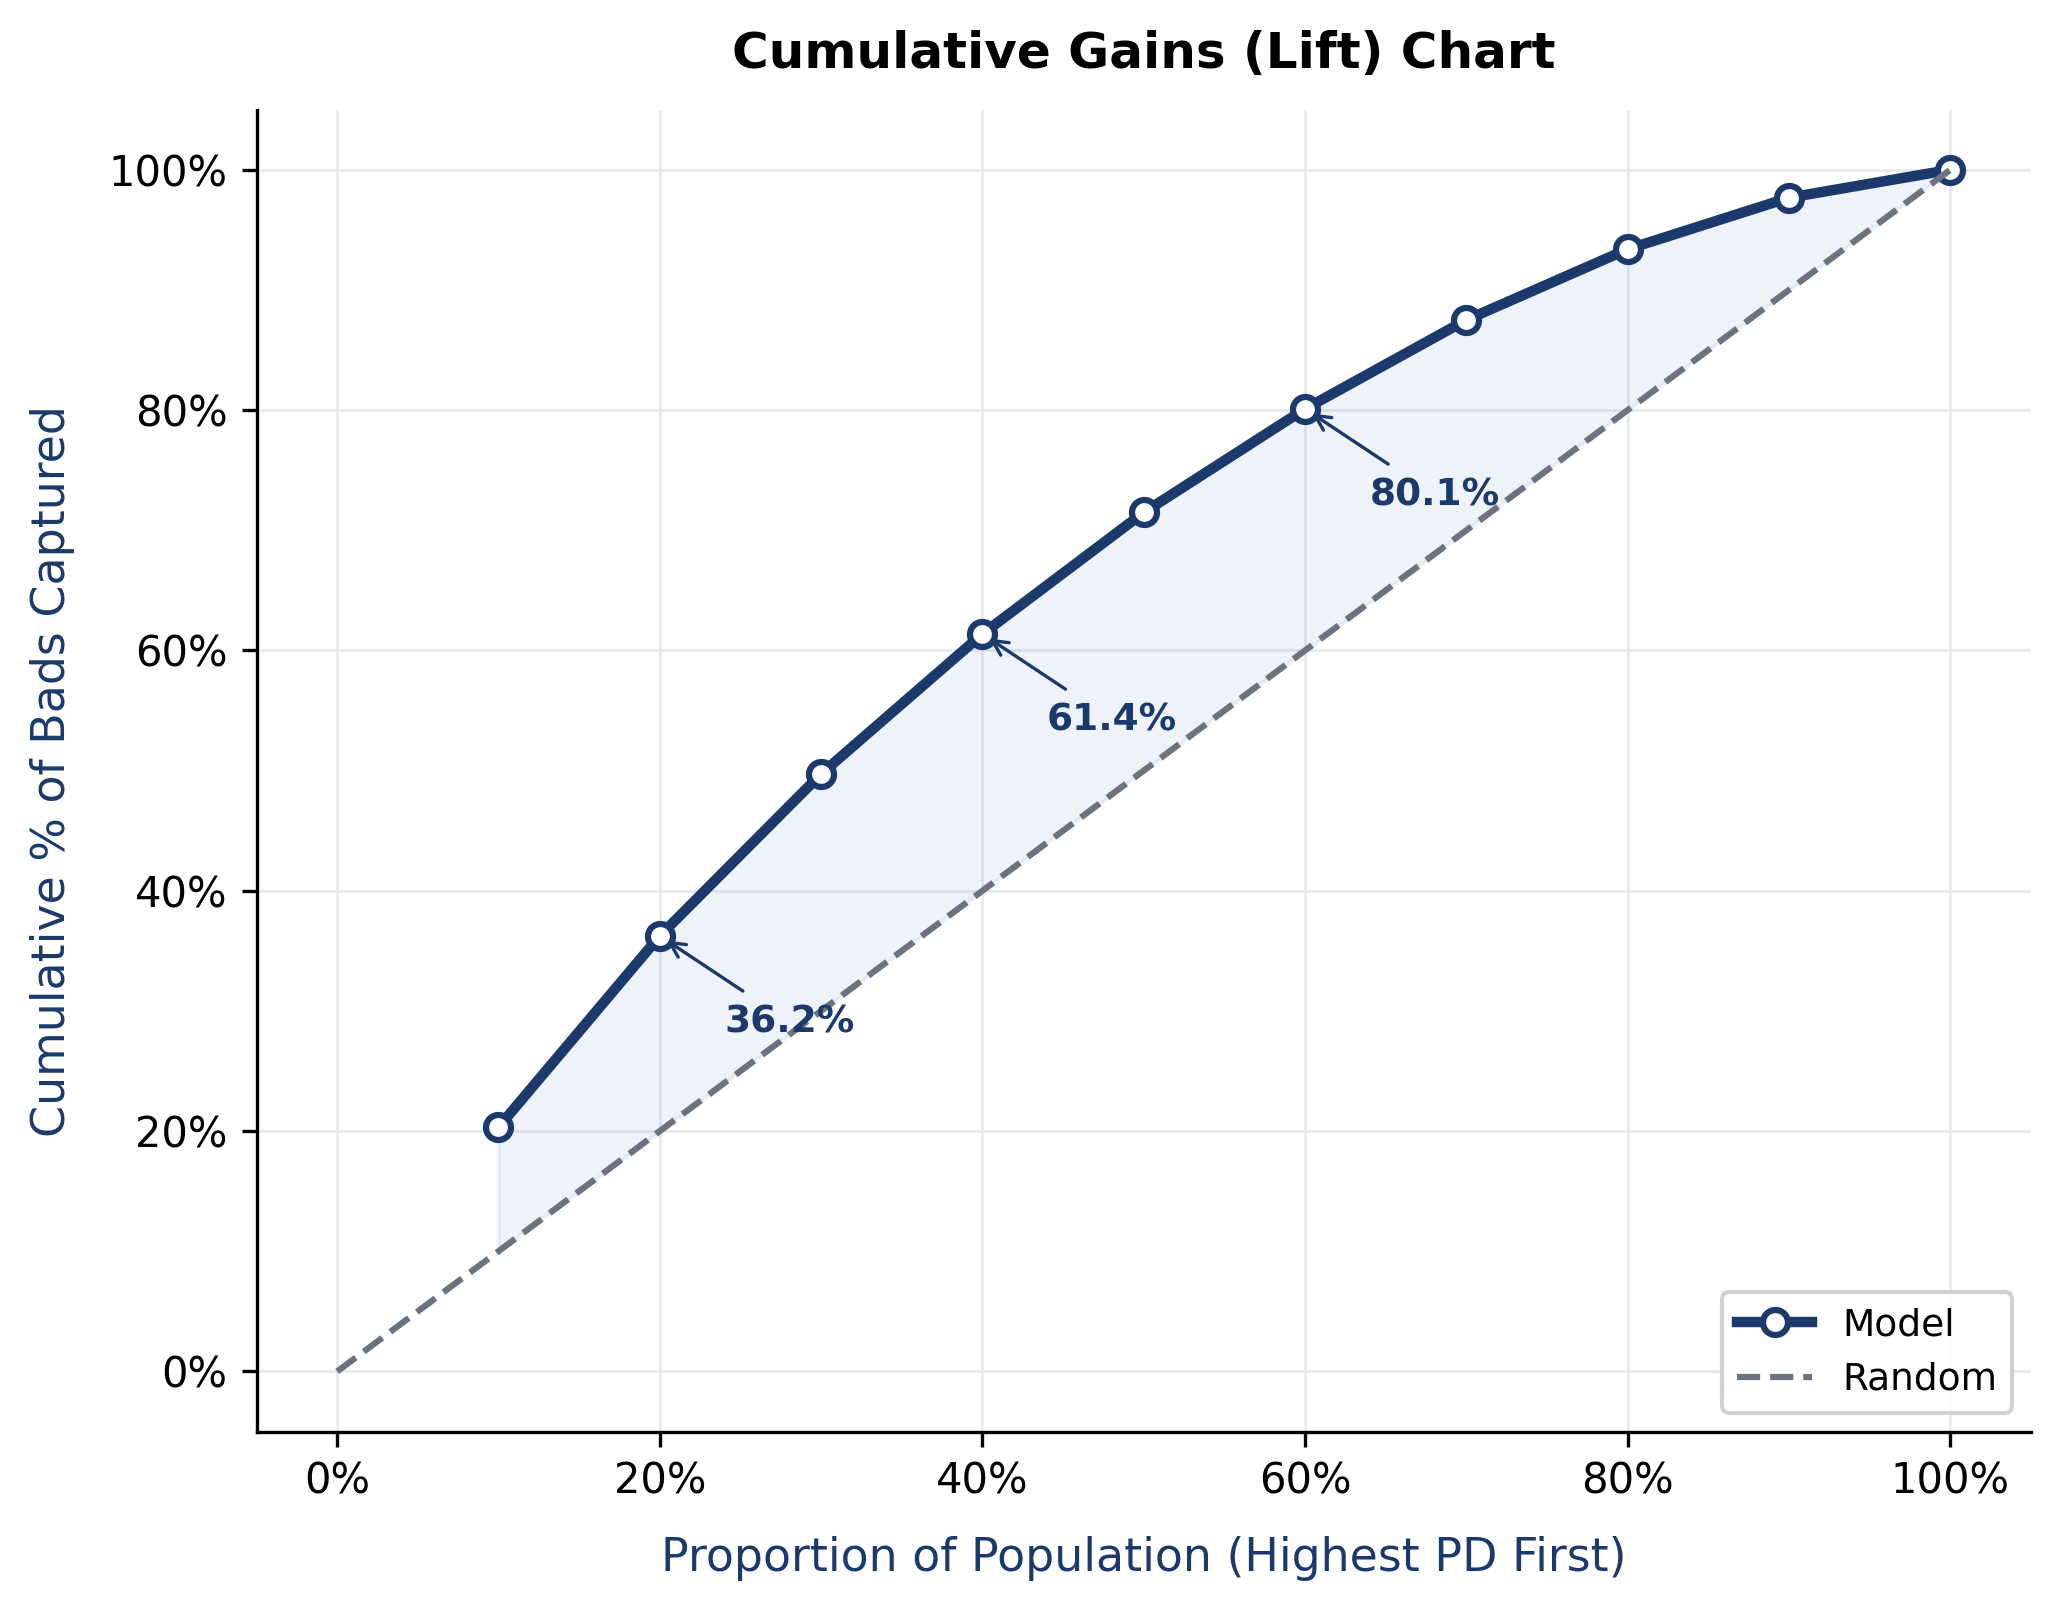
\includegraphics[width=\textwidth]{figures/validation/gains_chart.png}
    \caption{Cumulative Capture (Gains) Chart --- \textbf{OOT partition}}
    \label{fig:gains_ch}
\end{subfigure}
\hfill
\begin{subfigure}[b]{0.49\textwidth}
    \centering
    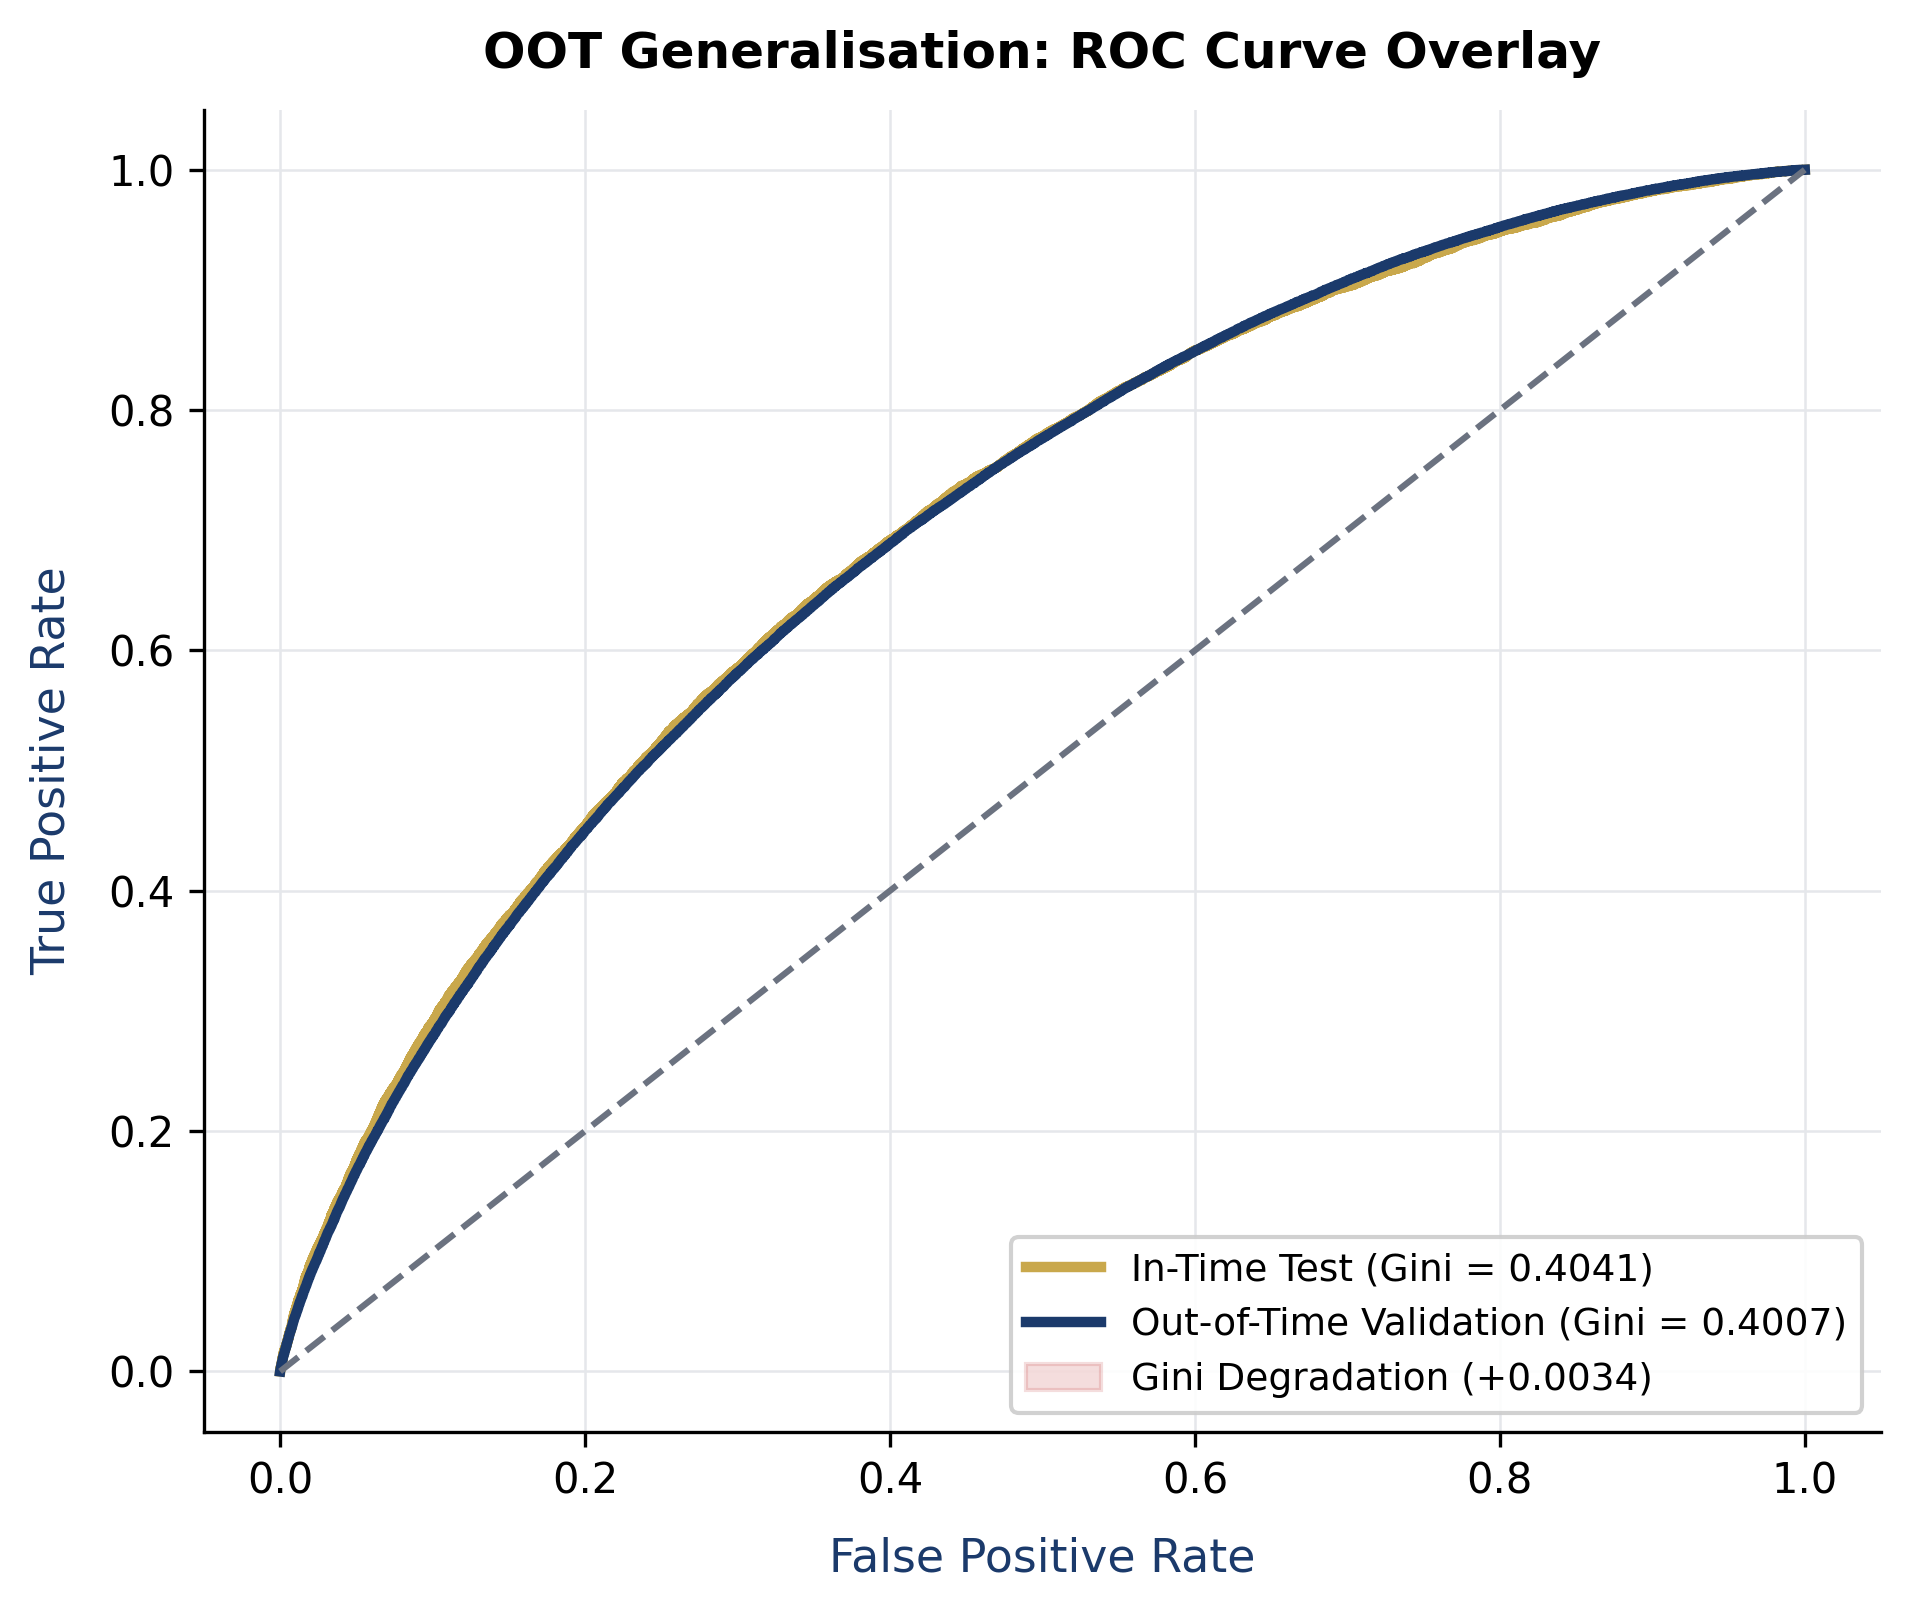
\includegraphics[width=\textwidth]{figures/validation/roc_oot_overlay.png}
    \caption{ROC Curve (Holdout vs OOT Overlay)}
    \label{fig:roc_overlay}
\end{subfigure}
\caption{Lift and Generalisation Overlays}
\label{fig:lift_overlays}
\end{figure}

% -----------------------------------------------------------------------------
% 9. LIMITATIONS AND RECOMMENDATIONS
% -----------------------------------------------------------------------------
\section{Business Decisioning and Cutoff Optimisation}

Underwriting decisions require balancing credit risk, portfolio growth, and capital constraints. We evaluate each score cutoff on Expected Profit and Risk-Adjusted Return on Capital (RAROC), with expected loss (at the approved-population bad rate) and a 12.00\% cost-of-capital charge on economic capital both netted out. On this portfolio the unconstrained RAROC-maximising cutoff sits at the most \emph{exclusive} non-empty cutoff on the grid (score \textbf{610}, approving only \textbf{0.002\%} of the population at a RAROC of \textbf{180.71\%}) --- RAROC is a ratio to economic capital, so it is maximised by the smallest, best-quality approved book regardless of whether that book is worth writing; the profit argmax sits instead at cutoff \textbf{480} (approving \textbf{99.89\%}). Because neither unconstrained optimum is an operating point (one approves almost nobody; the other approves almost everybody, at an approved bad rate of \textbf{21.48\%}), the decision problem is formulated as a \emph{constrained} optimization: we maximize approved volume and expected profit subject to an active risk-appetite ceiling on the approved bad rate (\textbf{15.00\%}), taking the most inclusive cutoff (maximising approved profit) whose approved bad rate stays within that ceiling. This constrained boundary represents the recommended operating cutoff.

We sweep score cutoffs from 400 to 800 (evaluating approved loan subsets) to calculate Expected Profit and RAROC. All components are expressed on a consistent \emph{per-annum} basis:
\begin{itemize}
    \item \textbf{Interest Income:} Based on per-loan interest rates (annual coupon on EAD).
    \item \textbf{Fees:} 1.0\% of Exposure at Default (EAD) per annum.
    \item \textbf{Funding Cost:} 4.0\% of EAD per annum.
    \item \textbf{Operating Cost:} 1.5\% of EAD per annum.
    \item \textbf{Expected Loss (EL):} $\text{PD}_{\text{annual}} \times \text{LGD} \times \text{EAD}$, where the lifetime PD is converted to an annual default probability via $\text{PD}_{\text{annual}} = 1 - (1 - \text{PD}_{\text{lifetime}})^{12/\text{term}}$. Charging the full lifetime PD against a single year of income would overstate losses by the loan term and distort every cutoff decision.
    \item \textbf{Capital Cost:} the \textbf{cost of capital}, 12.00\%, charged against economic capital (the Minimum Capital Reserve, 8\% of RWA). This is distinct from the \textbf{RAROC hurdle} of 15.00\%, which is not a charge but the threshold the resulting RAROC is compared against. The two rates are different numbers with different roles and are used consistently as such throughout this section.
\end{itemize}

Table~\ref{tab:cutoff_raroc} displays the optimization results across selected score cutoffs.

\begin{table}[H]
\centering
\caption{Cutoff Strategy and Profitability Analysis (RAROC). The recommended operating cutoff --- the most inclusive score over the full 400--800 grid (step 10) whose approved bad rate stays within the risk-appetite ceiling --- is highlighted in bold.}
\label{tab:cutoff_raroc}
\vspace{0.5em}
\begin{tabular}{cccccc}
\toprule
\textbf{Cutoff Score} & \textbf{Approval Rate} & \textbf{Bad Rate} & \textbf{Expected Profit} & \textbf{Expected Loss} & \textbf{RAROC} \\
\midrule
500 & 95.5\% & 20.14\% & \$52,748,942 & \$229,870,931 & 24.38\% \\
\textbf{530} & \textbf{64.3\%} & \textbf{14.20\%} & \textbf{\$15,218,331} & \textbf{\$83,444,217} & \textbf{19.22\%} \\
540 & 47.2\% & 11.50\% & \$7,354,670 & \$45,910,055 & 17.27\% \\
580 & 3.7\% & 3.43\% & \$41,673 & \$1,136,738 & 12.45\% \\
620 & 0.0\% & 0.00\% & \$0 & \$0 & 0.00\% \\
660 & 0.0\% & 0.00\% & \$0 & \$0 & 0.00\% \\
700 & 0.0\% & 0.00\% & \$0 & \$0 & 0.00\% \\
\bottomrule
\end{tabular}
\end{table}

As shown in the table, the recommended operating cutoff is score \textbf{530} with an approval rate of \textbf{64.34\%}, a bad rate of \textbf{14.20\%}, an expected profit of \textbf{\$15.2M}, and a RAROC of \textbf{19.22\%} --- above the 15.00\% RAROC hurdle. It is the most inclusive cutoff whose approved bad rate stays within the risk-appetite ceiling, and it appears as the highlighted row in Table~\ref{tab:cutoff_raroc} and is marked in Figure~\ref{fig:cutoff_profit}. A single objective drives the highlighted table row, the figure, and this text, so there is no discrepancy between the quoted cutoff and the swept grid. Relaxing the risk-appetite ceiling lowers the cutoff and raises approved volume; tightening it raises the cutoff toward the near-zero-volume unconstrained corner. 19 of the 22 non-empty cutoffs on the 400--800 grid clear the 15.00\% hurdle, the strongest being cutoff 610 at a RAROC of 180.71\%; the operating point trades some of that return for the risk-appetite ceiling on the approved bad rate.

\begin{figure}[H]
\centering
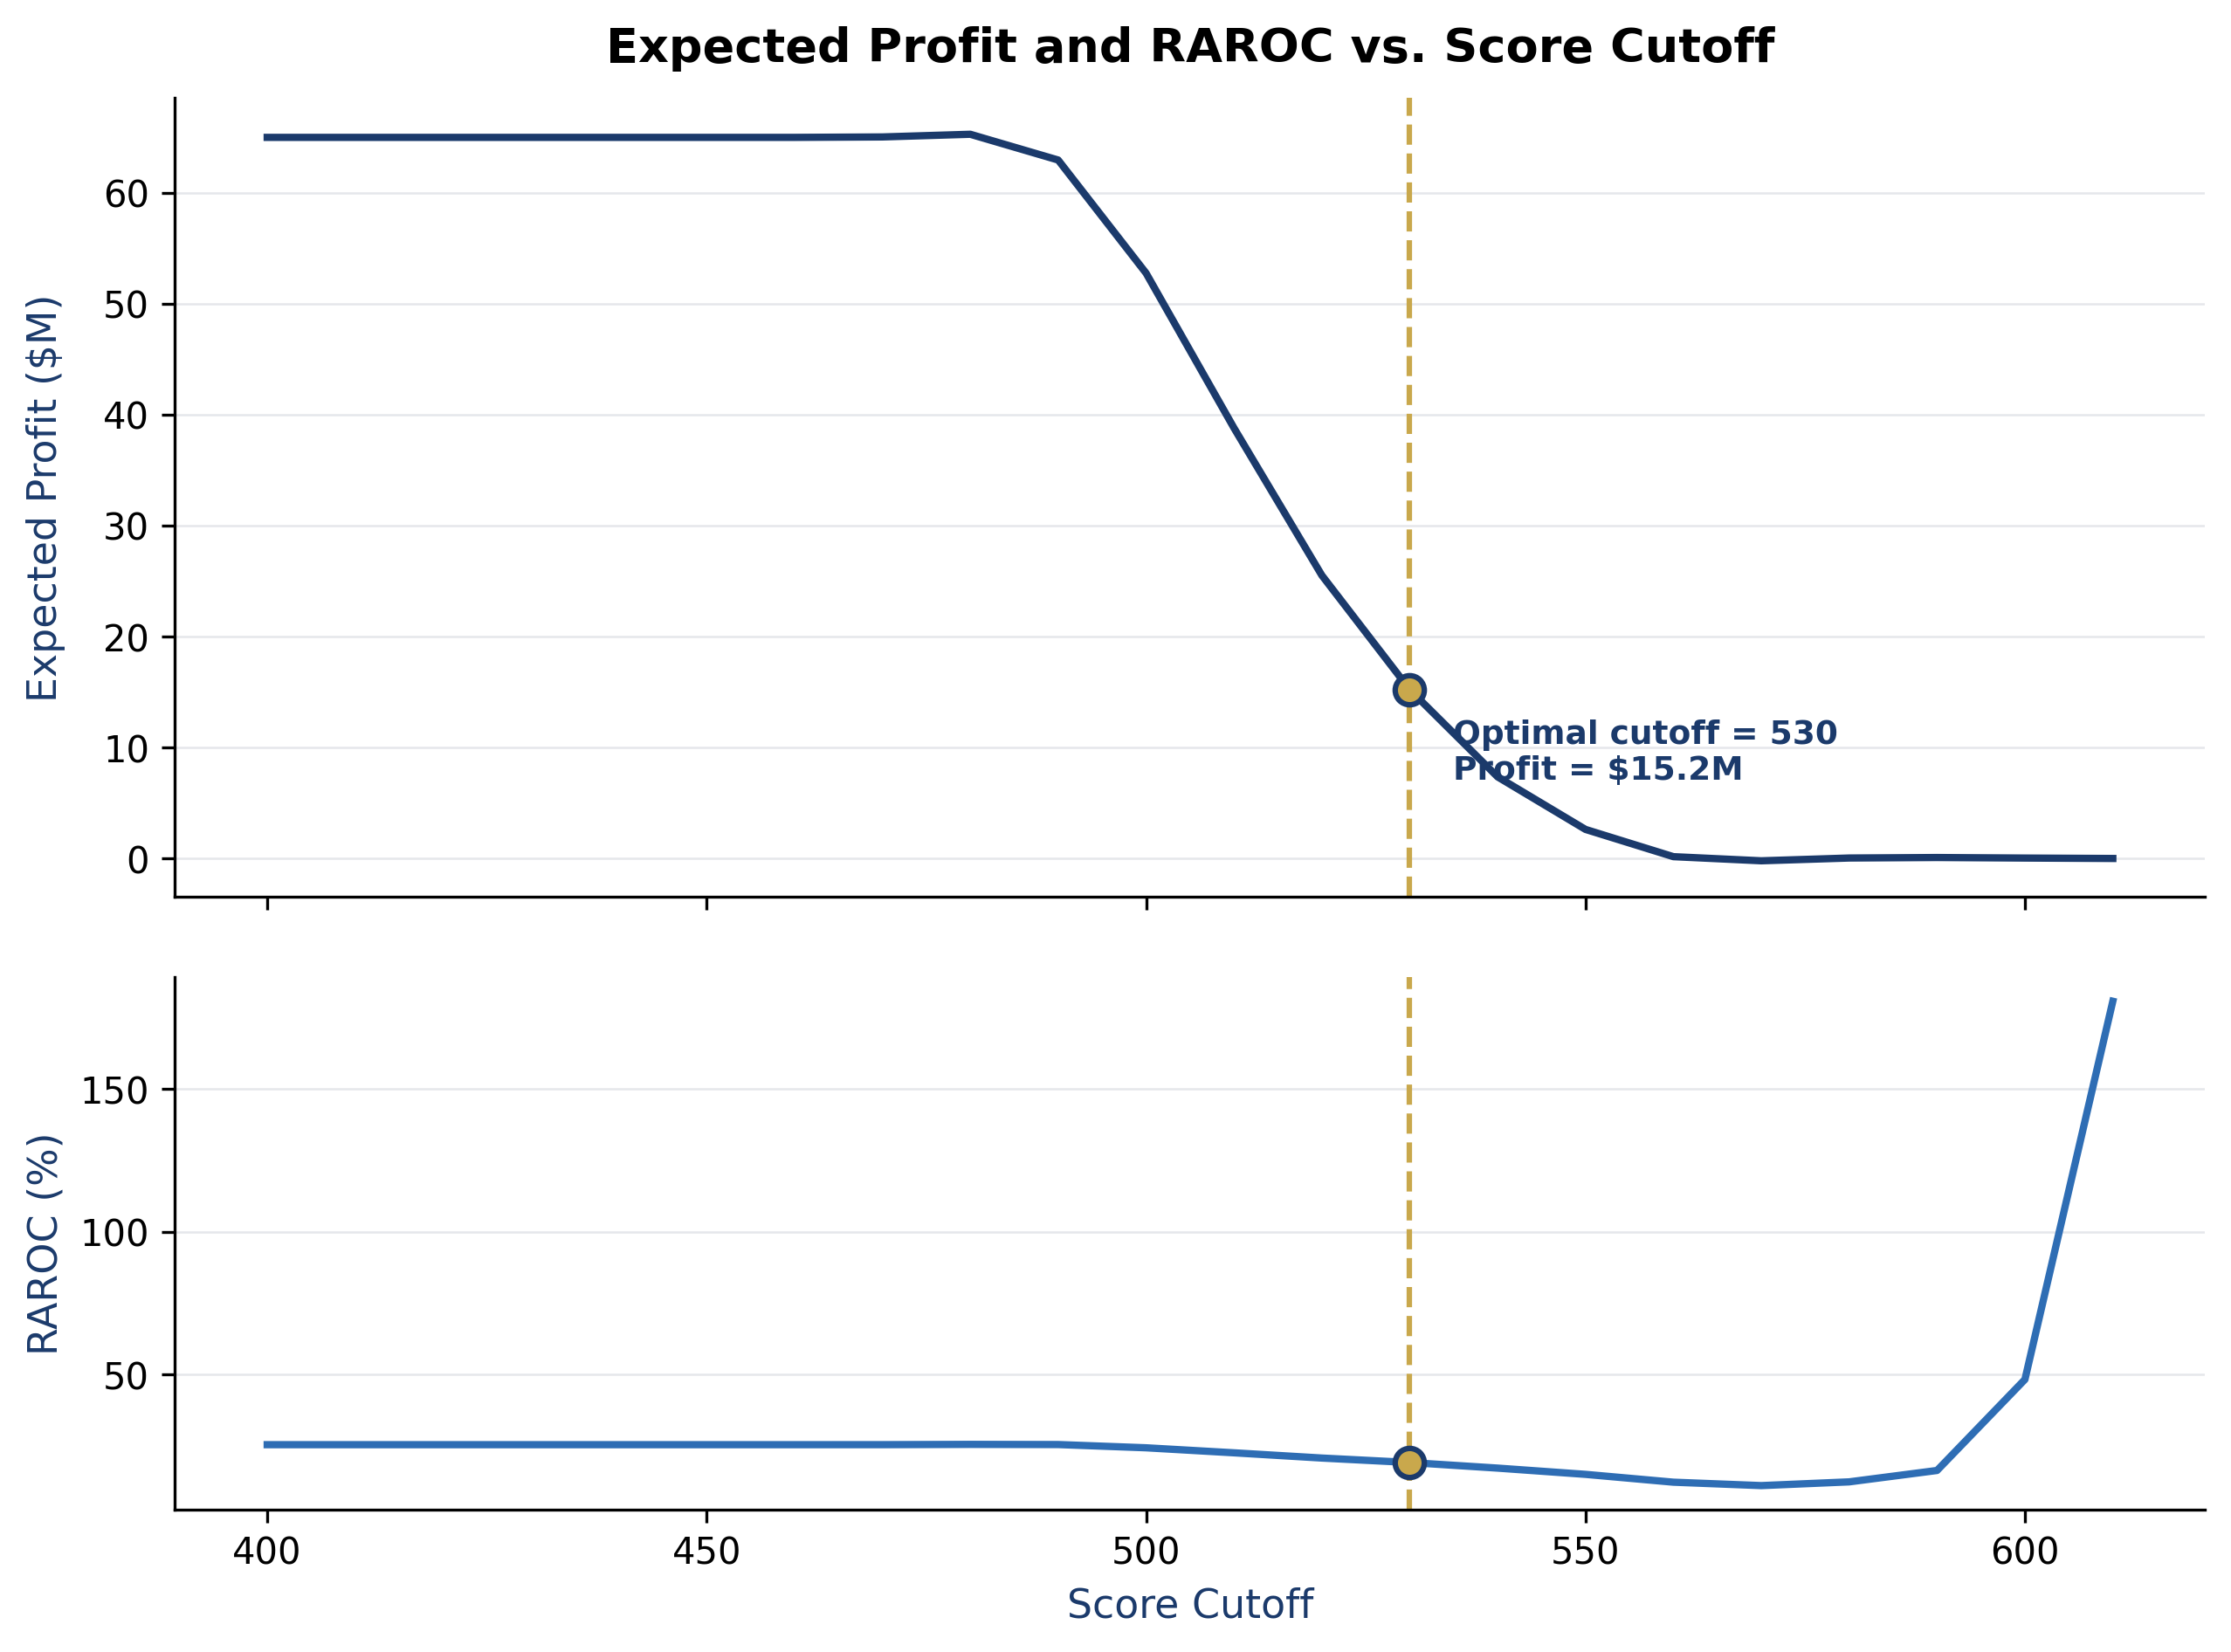
\includegraphics[width=0.68\textwidth]{figures/cutoff_profit_curve.png}
\caption{Expected Profit and RAROC versus score cutoff over the full 400--800 grid. The gold marker denotes the recommended operating cutoff (risk-appetite ceiling on the approved bad rate) reported in Table~\ref{tab:cutoff_raroc}.}
\label{fig:cutoff_profit}
\end{figure}

\section{Limitations, Assumptions, and Recommendations}
\label{sec:assumptions}

\subsection{Model Risk \& Limitations}
The Lending Club dataset is limited to US consumer loans and may not generalize to corporate lending, small-business loans, or other international retail portfolios. Additionally, the dataset excludes collateral details, meaning the LGD model relies primarily on underwriting grades and debt-to-income (DTI) metrics.

\subsection{Reconciling Expected Loss with IFRS~9 ECL}
The report carries two headline provisions --- the one-year Expected Loss of Section~5.2 and the IFRS~9 ECL of Section~6 --- defined over different horizons, with different staging, and with different discounting. The ECL is 4.8$\times$ the Expected Loss, and the gap is the staging: a lifetime horizon on Stage~2 and $PD=1$ on Stage~3 against a flat one-year horizon with no staging at all. Table~\ref{tab:el_ecl_reconciliation} decomposes both by stage, which makes the actual driver visible.

\begin{table}[H]
\centering
\small
\caption{Reconciliation: one-year Expected Loss vs.\ IFRS~9 ECL}
\label{tab:el_ecl_reconciliation}
\vspace{0.5em}
\begin{tabular}{lrrrrr}
\toprule
\textbf{Stage} & \textbf{Loans} & \textbf{EAD} & \textbf{Mean PD (12m, haz.)} & \textbf{Mean PD (life)} & \textbf{ECL} \\
\midrule
Stage 1 (12-month ECL) & 480,720 & \$1.24bn & 2.38\% & 11.24\% & \$0.03bn \\
Stage 2 (lifetime ECL) & 298,277 & \$1.32bn & 5.07\% & 24.65\% & \$0.28bn \\
Stage 3 (credit-impaired) & 213,664 & \$1.17bn & 5.01\% & 24.01\% & \$1.04bn \\
\midrule
\textbf{Total IFRS 9 ECL} & & & & & \textbf{\$1.35bn} \\
\textbf{One-year Expected Loss} & & & & & \textbf{\$0.28bn} \\
\bottomrule
\multicolumn{6}{p{0.92\linewidth}}{\footnotesize \textit{Note:} the ECL is 4.8$\times$ the one-year Expected Loss. That is a gap between two differently-defined quantities, not a discrepancy. Expected Loss is $PD_{\text{12m}} \times LGD \times EAD$ over one year, undiscounted and with no staging. ECL applies a 12-month horizon to Stage~1, a lifetime horizon to Stage~2, and $PD = 1$ to Stage~3, discounts at the effective interest rate, and probability-weights across macro scenarios. The Stage~3 column dominates both, and in that column the PD model plays no part at all (Section~10.3). The two PD columns come from the \emph{hazard} term-structure model, which is what drives the staged ECL; the one-year Expected Loss row is built from the \emph{scorecard}'s annualised PD instead, so the 12-month column does not multiply out to the EL total.} \\
\end{tabular}
\end{table}

\subsection{Stage 3 Is a Hindsight Classification, and It Dominates the ECL}
The single most material limitation of this engine concerns \emph{what the headline ECL figure actually measures}. IFRS~9 Stage~3 (credit-impaired) is normally identified by observed non-performance --- 90+ days past due at the reporting date. The LendingClub accepted-loan file is loan-level with no monthly delinquency panel, so no such observation exists. The implementation therefore classifies Stage~3 from the loan's \emph{terminal resolved status} --- the same variable used as the PD modelling target. Stage~3 membership is consequently known only with hindsight, and each Stage~3 loan is provisioned at $\text{LGD}\times\text{EAD}$ with PD forced to $1.0$, a quantity entirely insensitive to the PD model.

The what-if calculator in Section~7.6 makes the resulting dominance measurable. Shocking LGD by $+10$pp moves the total ECL by +11.1\% and shocking EAD by $+15\%$ moves it by +15.0\% --- both exactly proportional, as they must be, since ECL is linear in each. But shocking PD by $+50\%$ moves it by only +9.9\%. If a fraction $f$ of the ECL sits in the PD-independent Stage~3 term, a $+50\%$ PD shock produces a change of $0.5\,(1-f)$; the observed sensitivity therefore implies $f \approx$ 80\% of the reported provision. The what-if base is \$1.30bn: a single-scenario ECL at $Z=0$, 3.6\% away from the probability-weighted headline of \$1.35bn. The inference above is a ratio of shocks to that same base, so the anchor cancels.

In other words, the headline ECL is, to first order, \emph{realised defaults} $\times$ \emph{LGD} $\times$ \emph{EAD} --- an accounting identity computed with knowledge of the outcome --- and every forward-looking component of the engine (the macro regression, the Vasicek $Z$-shocks, the probability-weighted scenarios and the hazard term structure) moves only the residual. The Stage~1 and Stage~2 provisions, the ECL coverage ratio on the performing book, and the macro sensitivity analysis remain meaningful as relative comparisons; the absolute headline provision should not be read as a forward-looking estimate of losses on an unresolved portfolio. A production deployment on a live book, where Stage~3 is set by observed delinquency at the reporting date rather than by terminal outcome, would not have this property.

\subsection{Known Model Assumptions and Limitations}
This single list carries every model assumption and its associated limitation; it replaces the separate assumptions table that previously restated several of these items in shorter form.
\begin{itemize}
    \item \textbf{PD scorecard --- coarse monotone WoE bins:} Binning is monotone by construction, so genuinely non-monotone relationships are flattened rather than fitted. The tree challengers in Section~3.6 bound what that costs: they are free to fit non-monotone structure and do not materially outperform.
    \item \textbf{LGD --- portfolio-level validity only:} The deployed severity model is selected on out-of-sample error, with EAD proxied by \texttt{funded\_amnt} so accrued interest is ignored. Loan-level $R^2$ is negative, so LGD predictions are used for portfolio aggregates and must not be read as per-loan estimates.
    \item \textbf{EAD --- closed-form annuity, no prepayment:} Exposure is the contractual amortisation balance; borrowers who prepay are therefore carried at a higher exposure than they actually hold. This is conservative for capital. Months on book is measured as elapsed time from origination to the reporting date, capped at the contractual term, so exposure declines with loan age as it should.
    \item \textbf{Hazard --- constant within each calendar month:} The discrete-time formulation holds the hazard flat inside each month, so intra-month seasoning is not represented; the monthly resolution is what bounds this, and it is finer than the annual step a Markov-chain alternative would impose.
    \item \textbf{Basel IRB --- single systematic factor:} The ASRF ``Other Retail'' supervisory correlation $R \in [0.03, 0.16]$ assumes one common factor, so name and sector concentration are not captured. Section~5.3 reports the concentration diagnostics separately.
    \item \textbf{Reject inference --- sampled rejects:} Parcelling runs on a 100k random sample of the 27.6M reject rows, so the sample may not represent the full reject distribution; the Gini shift is monitored rather than assumed stable.
    \item \textbf{No stage-migration matrix:} A 12-month stage transition matrix requires the stage a loan occupied at a past date, which needs a monthly servicing panel this dataset does not contain. Section~7.5 sets out why no such matrix is reported rather than reconstructing one.
    \item \textbf{No origination-date PD snapshot --- relative SICR trigger disabled:} IFRS~9's primary SICR test compares the current lifetime PD against the PD estimated \emph{at booking}. This dataset stores no booking-date model output, so no such snapshot exists. Rather than substitute the current PD for the origination PD --- which makes the ratio identically $1.0$ and silently disables the test while appearing to implement it --- the relative trigger is switched off and Stage~2 is driven by the absolute lifetime-PD threshold and the delinquency backstop alone. Reinstating it requires storing PD at booking, which is listed under Recommended Next Steps below.
    \item \textbf{Delinquency backstop is an application-time proxy:} The implemented backstop is \texttt{delinq\_2yrs} $\geq 1$ --- delinquencies in the two years \emph{before} origination --- not the IFRS~9 standard 30+ DPD at the reporting date, which this data cannot support.
    \item \textbf{Downturn LGD sits at the distribution cap:} The Basel downturn LGD is the 90th percentile of the \emph{realised} severity of loss-incurring defaults, which on this fully unsecured, non-revolving book is 1.0000 --- the upper bound of the $[0,1]$ range. It is a genuine empirical percentile rather than a modelled stress, and it cannot be exceeded, so the capital calculation carries no headroom above it for a severity worse than total loss.
    \item \textbf{Hazard-model event timing is a proxy:} The data records no observed default \emph{date}, so the discrete-time hazard panel is built against a duration proxy --- cumulative payments divided by the contractual instalment --- and right-censors survivors at the month their payments stop. This is the same proxy the Kaplan-Meier/Cox challenger in Section~3.7 uses. It replaces an earlier construction that gave every loan its full contractual term of person-periods with the event pinned to the final one and no censoring; that version fitted a 12-month hazard of essentially zero, which provisioned the entire Stage~1 book at nil. The remaining limitation is that the duration is inferred, not observed, and that prepayment is treated as censoring rather than as a competing risk --- so a borrower who repays early is treated as having survived to that point rather than as having left the risk pool for a different reason.
    \item \textbf{Portfolio aggregates are partly in-sample:} Expected Loss, Basel RWA and IFRS~9 ECL are computed over the combined train, in-time test and OOT partitions --- the same rows the scorecard, hazard and LGD models were fitted on. This is appropriate for provisioning a closed book but means the portfolio aggregates are not out-of-sample quantities; the out-of-sample evidence is the OOT discrimination and calibration in Section~7.
    \item \textbf{The out-of-time sample is selected on maturity, not drawn at random:} the modelling population keeps only loans whose status is resolved at the 2018Q4 snapshot, so 2016--2018 originations that were still \emph{Current} are excluded. Among recent vintages the loans that have already resolved are disproportionately those that ended early --- that is, the charged-off ones --- and 60-month loans are under-represented relative to 36-month ones. The effect is visible in the composition of the window: half the OOT observations come from the eleven months to \textbf{2016-11} and the other half from the following twenty-five, over a period when origination volume was rising. Every OOT statistic in Section~7 (AUC, KS, PSI, Hosmer-Lemeshow, and the recalibration gate that keys off them) inherits this selection.
    \item \textbf{Exposure is booked on loans that no longer exist:} EAD amortises each loan contractually to the \textbf{2018-12-31} reporting date from its origination month, but a large part of the book had already been repaid in full or charged off years before that date, and their true exposure at the reporting date is zero. Stage~3 in particular ($\text{EAD} =$ \$1.17bn) consists by construction of loans whose terminal status is already known. The zero-prepayment assumption noted above covers early repayment \emph{within} a live loan; it does not cover provisioning against exposures that had already terminated. The engine should be read as pricing this book as if observed at origination-plus-elapsed-term, not as a snapshot of a live portfolio.
    \item \textbf{The macro apparatus is fitted on the training window only:} the OLS default-rate regression, the scenario projections, the implied Vasicek $Z$ shocks, the ADF / Granger / Johansen diagnostics and the PiT--TTC decomposition are all estimated on the \emph{training} vintages (2007--2014), four years before the reporting date, and then applied to the whole book. Nothing in the 2016--2018 era informs the macro sensitivities that drive the forward-looking part of the ECL.
    \item \textbf{Constant exposure inside the ECL sum:} $\text{LGD}(t)$ and $\text{EAD}(t)$ are held at their per-loan point estimates across the ECL horizon rather than re-amortised monthly, which is conservative for amortising loans.
    \item \textbf{The adverse scenario is a rate-and-inflation shock, not a lower-bound recession:} Every macro axis moves in the direction its imposed sign prior says raises defaults (downside) or lowers them (upside), so the required Downside $>$ Baseline $>$ Upside ordering holds \emph{by construction} for any non-negative coefficient magnitudes rather than depending on the fitted values. The consequence is that the downside tightens policy and raises inflation into the downturn. This is a deliberate choice: it is the more punitive configuration for an unsecured consumer book, where floating debt-service costs and a real-income squeeze compound the unemployment shock, and it matches how supervisory adverse scenarios are typically built. A deflationary lower-bound recession, in which policy is cut, would instead \emph{offset} part of the adverse shock through the rate channel and is not modelled here.
    \item \textbf{The ``baseline'' scenario maps to $Z = $ -0.1915, not $Z=0$:} This is a property of the Vasicek conditional-PD function, whose value at $Z=0$ does not equal the unconditional PD; the projection intercept is recentred so the baseline reproduces the through-the-cycle default rate. Under the report-wide convention that $Z<0$ is adverse, the baseline therefore reads as mildly adverse even though it is the central expectation.
    \item \textbf{Categorical Feature Encoding:} Grade, term, employment length and home ownership are ordinal-encoded before WoE binning. Label ordering assumptions (e.g., A=1 through G=7) are reasonable but should be validated against observed default rates for each category.
\end{itemize}

\subsection{Empirical Results vs.\ Published Literature}
\label{subsec:benchmarks}

\begin{table}[H]
\centering
\footnotesize
\setlength{\tabcolsep}{2.5pt}
\caption{Project empirical results vs.\ published reference ranges (comparison against the literature, not a reproduction of the cited studies).}
\label{tab:literature_benchmarks}
\begin{tabularx}{\linewidth}{p{2.2cm}ccp{2.2cm}lp{4.5cm}}
\toprule
\textbf{Metric} & \textbf{This Study} & \textbf{Published Range} & \textbf{Source} & \textbf{Verdict} & \textbf{Comment}\\
\midrule
Scorecard Gini (OOT) & 0.4007 & $0.30 - 0.45$
  & \cite{lessmann2015benchmarking} & Within range & \\
LightGBM Gini (OOT)  & 0.4067 & $0.35 - 0.55$
  & \cite{lessmann2015benchmarking} & Within range & \\
Mean LGD (P2P)       & 0.8931 & $0.25 - 0.45$
  & \cite{bellotti2012} & Above typical range & The OOS-validated LightGBM severity model puts mean LGD above both cited bands, consistent with low post-charge-off recovery on unsecured instalment loans once EAD is principal-only; the rejected two-stage model materially under-predicted severity (OOS $R^2 \approx -2.70$) \\
Downturn LGD         & 1.0000 & $0.25 - 0.45$
  & \cite{bellotti2012} & Above typical range & Conservative 90th-percentile downturn uplift above the mean band \\
IFRS~9 ECL Coverage  & 36.210\% & 40\% -- 45\%
  & \cite{eba2022} & Below typical range & The published band is the EBA \emph{NPL} coverage ratio (allowance on \emph{non-performing} exposure only); the project figure is whole-book lifetime ECL over total EAD, which blends performing Stage~1 exposure and therefore sits below impaired-only coverage --- not a like-for-like gap \\
IFRS~9 Stage~2\%     & 30.0\% & 8\% -- 11\%
  & \cite{eba2022} & Above typical range & Stage~2 share well above the EBA EU-aggregate ($\approx$9--10\%): expected for an unsecured, high-yield US consumer book with materially higher SICR incidence than the diversified EU bank averages \\
\bottomrule
\end{tabularx}
\end{table}

\footnotesize\noindent Verdicts in Table~\ref{tab:literature_benchmarks} are recomputed at every build by numerical comparison of the two adjacent columns; out-of-range values are reported as such, with the driver noted in the Comment column.\normalsize

\subsection{Recommended Next Steps}
\begin{enumerate}
    \item \textbf{Independent Validation:} Conduct an independent review of the binning algorithms and scorecard points scaling to verify math and logical consistency.
    \item \textbf{Advanced LGD Modeling:} Explore survival-based LGD models that capture time-varying recovery patterns over the life of defaulted assets.
    \item \textbf{Longitudinal SICR Tracking:} Implement a proper SICR framework using origination-date PD snapshots stored at booking, enabling precise Stage 2 migration rates compliant with IFRS 9 paragraph 5.5.9.
\end{enumerate}

\clearpage
% -----------------------------------------------------------------------------
% 10. APPENDICES
% -----------------------------------------------------------------------------
\section{Appendices}

\subsection{A. Scorecard Scaling Derivation}
To map the log-odds predicted by the logistic regression to a scaled credit score, we solve the linear system:
\begin{equation}
Score = Offset + Factor \times \ln(\text{odds})
\end{equation}
Subject to the boundary conditions:
\begin{itemize}
    \item $\text{Score} = 600$ at $\text{odds} = 50:1$ ($\ln(50) \approx 3.912$)
    \item $\text{Score} = 620$ at $\text{odds} = 100:1$ ($\ln(100) \approx 4.605$, satisfying $\text{PDO} = 20$)
\end{itemize}
Solving for the scaling parameters:
\begin{equation}
Factor = \frac{20}{\ln(100) - \ln(50)} = \frac{20}{\ln(2)} \approx 28.8539
\end{equation}
\begin{equation}
Offset = 600 - 28.8539 \times \ln(50) \approx 487.123
\end{equation}

\subsection{B. Basel IRB ``Other Retail'' Supervisory Parameters}
Under BCBS §322--328 the regulatory correlation $R$ is constrained to $[0.03, 0.16]$ and decays exponentially as PD rises, reflecting the lower correlation of defaults among higher-risk borrowers in stable conditions; the formula is stated in Section~5.1 and is not repeated here. For the RWA calculation the supervisory PD floor of \textbf{0.03\%} is strictly applied, and the PD entering it is the twelve-month measure derived in Section~5.1.

\subsection{C. Technical Stack \& Reproducibility}
The pipeline is designed to be fully reproducible:
\begin{table}[H]
\centering
\caption{Modeling Pipeline Technology Stack}
\label{tab:tech_stack}
\vspace{0.5em}
\begin{tabular}{p{3.2cm}p{4.0cm}p{6.8cm}}
\toprule
\textbf{Component} & \textbf{Technology} & \textbf{Purpose in Pipeline} \\
\midrule
Language & Python 3.11+ & Core language and scripting \\
Feature Binning & \texttt{optbinning} \texttt{BinningProcess} & WoE bin construction for every scorecard feature \\
PD Underwriting & statsmodels Logit & Monotonic credit scorecard fitting \\
Feature Selection & scikit-learn \texttt{LogisticRegressionCV} (ElasticNet, SAGA) & Third selection stage, between the VIF filter and the sign check (Section~3.3) \\
LGD Modeling & LightGBM (deployed); scikit-learn \texttt{GradientBoostingClassifier} (cure stage); statsmodels GLM (severity stage) & Severity model selected out-of-sample; the two-stage cure + fractional-logit model is the benchmarked \emph{challenger} that was not deployed (Section~4.2) \\
Challenger Models & LightGBM, XGBoost, scikit-learn \texttt{RandomForest} & Non-linear machine learning benchmarks (Table~\ref{tab:ml_comparison}) \\
Survival PD Curves & Discrete-time hazard model; \texttt{lifelines} Cox challenger & Monthly lifetime term structure modeling \\
PDF Generation & XeLaTeX + biber & Publication-quality academic PDF \\
\bottomrule
\end{tabular}
\end{table}

\noindent\textbf{Enhancement phases dropped in this run:} none. Every optional phase records a non-fatal failure if it does not complete, so a table that silently vanished from this report --- for example because an optional dependency was absent --- is disclosed here rather than simply being absent.

\vspace{0.6em}
\noindent\textbf{Computed but not tabulated here.} The pipeline also writes the OOT decile rank-ordering table, the LGD backtest by vintage, and the full ECL macro-sensitivity grid (shown here only as Figure~\ref{fig:ecl_tornado}) to \texttt{outputs/metrics.json}. They are omitted from the body for length, not because they were unfavourable; each is reproducible from that file without re-running the pipeline.


\clearpage
\section*{References}
\addcontentsline{toc}{section}{References}
\printbibliography[heading=none]

\end{document}
